\documentclass[a4paper, 12pt]{report}
\usepackage[utf8]{inputenc}
\usepackage{amsmath}
\usepackage{svg}
\usepackage[T1]{fontenc}
\usepackage[english]{babel}
\usepackage{datetime}				%makes your life with dates easier
\usepackage{geometry}
\usepackage{listings}
\providecommand*{\lstlistingautorefname}{Listing}
\usepackage{framed}					%used for framing of code listing in appendix
\usepackage{color}
\usepackage{float}
\usepackage{graphicx}
\usepackage{caption}					%centering captions
\usepackage[acronym]{glossaries}
\usepackage{microtype}				%nicer spacing and fixes bad boxes in bibliography
\usepackage{minted}
\usepackage{csquotes}
\usepackage{multirow}
\usepackage[linesnumbered]{algorithm2e}
\usepackage{fancyvrb} %to allow cross-referencing in verbatim text
\usepackage{bytefield}
\usepackage{booktabs}
\usepackage{tabularx}
\usepackage{tabulary}
\usepackage{tikz}
\usepackage{enumitem}

\usepackage{colortbl}
\usepackage{hhline}

\usepackage{siunitx}


\usepackage{hyperref}
\usetikzlibrary{shapes.geometric, shapes.symbols, arrows.meta, positioning, calc, backgrounds,fit,positioning}

%%
% Simple Quantity,\qty{64}{\byte},64 B,Ensures a non-breaking thin space between number and unit.
% Bits,\qty{3}{\bit},3 b,Consistent font for the unit symbol.
% Written out,\qty[per-mode=symbol]{3}{bits},3 bits,"Useful if you prefer the word ""bits"" over ""b""."
% Binary Prefix (IEC),\qty{10}{\kibi\byte},10 KiB,Correctly distinguishes 1024 bytes (KiB) from 1000 (KB).
% Decimal Prefix,\qty{10}{\kilo\byte},10 kB,Standard decimal kilo (1000).
% Ranges,\qtyrange{8}{16}{\byte},8 B to 16 B,"Handles the range word (""to"") automatically."
%%

\sisetup{
    group-separator = {\,},
    group-minimum-digits = 4
}
\DeclareSIUnit\byte{B}
\DeclareSIUnit\bit{b}
\DeclareSIUnit\sat{sat}
\DeclareSIUnit\bitcoin{BTC}

% \qty{64}{\byte}	64 B 
% \qty{3}{\bit}	3 b
% \qty{10}{\kibi\byte}	10 KiB
% \qty{10}{\kilo\byte}  10 kB
% \qty{50}{\bitcoin}	50 BTC
% \qty{100000000}{\sat}	100,000,000 sat


\sisetup{
group-separator = {,},    % Uses comma for thousands (100,000)
group-minimum-digits = 4  % Starts grouping at 1000 (1,000)
}

%% ASCII art
\lstset{basicstyle={\ttfamily},literate={↓}{$\downarrow{}$}{1}}

%% Tikz configuration
\tikzset{
    dbtable/.style={
        draw, 
		thick, 
		rounded corners=2pt, 
		inner sep=0pt, 
		font=\footnotesize,
        align=left, 
    },
    relation/.style={
        -{Stealth[scale=1.2]}, thick, draw=gray!80
    }
}

\usepackage{verbatimbox}

%% Cusom commands for global style management
\newcommand{\service}[1]{\texttt{#1}}
\newcommand{\term}[1]{\textit{#1}}
\newcommand{\code}[1]{\texttt{#1}}
\newcommand{\tech}[1]{\textsc{#1}}
\newcommand{\file}[1]{\texttt{#1}}



%% This declares a command \Comment
%% The argument will be surrounded by /* ... */
\SetKwComment{Comment}{/* }{ */}

\RestyleAlgo{ruled} % to have lines around the algorithm and the caption

%%%%%%%%%%%%%%%%%title%%%%%%%%%%%%%%%


%%%%%%%%%%%%%listins%%%%%%%%%%%%%%%%%%%%%%%%%%%%%%%%
\usepackage[svgnames]{xcolor}
\definecolor{diffstart}{named}{Grey}
\definecolor{diffincl}{named}{Green}
\definecolor{diffrem}{named}{OrangeRed}

\definecolor{mygreen}{rgb}{0,0.6,0}
\definecolor{mygray}{rgb}{0.5,0.5,0.5}
\definecolor{mymauve}{rgb}{0.58,0,0.82}

\lstset{
	backgroundcolor=\color{white},   % choose the background color
	basicstyle=\footnotesize\ttfamily,        % size of fonts used for the code
	breaklines=true,                 % automatic line breaking only at whitespace
	captionpos=b,                    % sets the caption-position to bottom
	commentstyle=\color{mygreen},    % comment style
	escapeinside={\%*}{*)},          % if you want to add LaTeX within your code
	keywordstyle=\color{blue},       % keyword style
	stringstyle=\color{mymauve},	   % string literal style
	frame=single,
	float,
	stepnumber=1,
	numbers=left,
}
%%%%%%%%listing language for Patches
\lstdefinelanguage{diff}{ 
	basicstyle=\ttfamily\small,
	morecomment=[f][\color{diffstart}]{@@},
	morecomment=[f][\color{diffincl}]{+},
	morecomment=[f][\color{diffrem}]{-},
}

%%%%%%%%%%%%%%%%%%bibliography
\usepackage[backend=biber, style=ieee]{biblatex}
%\addbibresource{resources/zotero.bib}
\addbibresource{resources/bibliography.bib}

\setcounter{biburllcpenalty}{7000}
\setcounter{biburlucpenalty}{8000}

\makenoidxglossaries
% \newacronym{label}{Abbreviation}{Full Name}

\newacronym{ln}{LN}{Lightning Network}
\newacronym{utxo}{UTXO}{Unspent Transaction Output}
\newacronym{htlc}{HTLC}{Hash Time Lock Contract}
\newacronym{bolt}{BOLT}{Basis Of Lightning Technology}
\newacronym{lnd}{LND}{Lightning Network Deamon}
\newacronym{cln}{CLN}{Core Lightning}
\newacronym{ldk}{LDK}{Lightning Development Kit}
\newacronym{le}{LE}{Little-Endian}
\newacronym{be}{BE}{Big-Endian}
\newacronym{varint}{VarInt}{Variable Length Integer}
\newacronym{tlv}{TLV}{Type Length Value Format}
\newacronym{bigsize}{BigSize}{BigSize}
\newacronym{scid}{scid}{Short Channel ID}
\newacronym{wal}{WAL}{Write Ahead Log}
\newacronym{crc32}{CRC32}{Cyclic Redundancy Check 32-bit}
\newacronym{p2p}{P2P}{Peer-To-Peer}
\newacronym{pypi}{PyPI}{Python Package Index}
\newacronym{dto}{DTO}{Data Transfer Object}
\newacronym{isp}{ISP}{Internet Service Provider}
\newacronym{mpc}{MCP}{Multi Party Channel}
\newacronym{vtxo}{VTXO}{Virtual Transaction Output}
\newacronym{fibre}{FIBRE}{Fast Internet Bitcoin Relay Engine}
\newacronym{mvc}{MVC}{Model-View-Controller}
\newacronym{oom}{oom}{out-of-memory}
\newacronym{scd}{SCD}{Slowly Changing Dimension}
\newacronym{oltp}{OLTP}{Online Transaction Processing}
\newacronym{olap}{OLAP}{Online Analytical Processing}
\newacronym{vps}{VPS}{Virtual Private Server}
\newacronym{cdf}{CDF}{Cumulative Distribution Function}
\newacronym{bc}{BC}{Betweenness Centrality}
\newacronym{ram}{RAM}{Random Access Memory}
\newacronym{p2wsh}{P2WSH}{Pay-to-Witness-Script-Hash}
\newacronym{cli}{CLI}{Command Line Interface}
\newacronym{orm}{ORM}{Object Relational Mapper}
\newacronym{vpn}{VPN}{Virtual Private Network}
\newacronym{pcn}{PCN}{Payment Channel Network}

\begin{document}
	\pagenumbering{roman}
	%\maketitle
	\begin{titlepage} 
		\begin{centering}
			
			% Header
			\begin{figure}[!h]
				% TU Logo
				\begin{minipage}{0.3\linewidth}
					\begin{center}
						
\includegraphics[scale=0.8]{resources/images/tu-logo.eps} 
					\end{center}  
				\end{minipage}
                \hfill
				% ln-history Logo
                \begin{minipage}{0.3\linewidth}
					\begin{center}
						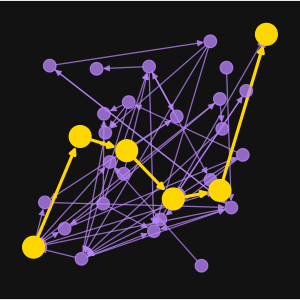
\includegraphics[scale=0.4]{resources/images/ln-history.png} 
					\end{center}  
				\end{minipage}
				\hfill
				% KBS Logo
				\begin{minipage}{0.35\linewidth} 
					\begin{center}
						
\includegraphics[scale=0.02]{resources/images/inet-logo.png} 
					\end{center}    
				\end{minipage}
			\end{figure}
			
			% vertikaler Zwischenraum
			\vspace{7mm}
			
			% Titel der Arbeit
			\LARGE
			
			Bachelorarbeit
			
			\textbf{Catching Lightning in a Database:}
            
			An Architecture for Real-Time Gossip Preservation
			\large
			
			% Name des Verfassers
			
			Fabian Kraus\\
			13. Mai 2026\\[3cm]
			
			% Betreuer
			\begin{minipage}{\linewidth} 
				\begin{tabbing}
					Betreuer: \quad \=Prof. Dr. Stefan Schmid\\ 
					Zweitgutachter: \quad \=Prof. Dr. Stefan Tai\\
                    Zweitbetreuer: \quad \=René Pickhardt\\
				\end{tabbing}
			\end{minipage}
			
			% vertikaler Zwischenraum
			\vfill
			
			\normalsize
			{Technische Universität Berlin}\\
			{Faklutät IV - Elektrotechnik und Informatik}\\
			{Institut für Telekommunikationssysteme}\\
			{Fachgebiet Intelligent Networks}\\
		\end{centering}
	\end{titlepage}
	
	\newpage
	\section*{Eidesstattliche Versicherung}
Hiermit erkläre ich, dass ich die vorliegende Arbeit selbstständig und eigenhändig sowie ohne 
unerlaubte fremde Hilfe und ausschließlich unter Verwendung der aufgeführten Quellen und Hilfsmittel 
angefertigt habe.\\
\\
Berlin, Date \\
\vspace{1cm}\\
\underline{\hspace{5cm}}\\
Name
	\newpage
	\section*{Zusammenfassung}

Die vorliegende Arbeit präsentiert \tech{ln-history}, eine neue Plattformarchitektur, 
die die Erfassung, langfristige Speicherung und tiefgreifende Analyse sowohl historischer 
als auch in Echtzeit erzeugten Gossip-Daten des Lightning Netzwerks, ermöglicht. 
Um diese Anforderungen an der Plattform zu demonstrieren, führt diese Arbeit 
eine empirische Analyse der Verbreitung von Gossip-Nachrichten sowie eine 
Untersuchung der topologischen Entwicklung des Netzwerks durch.

Durch den Aufbau eines der bislang vollständigsten Datensätze von Gossip-Nachrichten des Lightning Netzwerks  
etabliert diese Arbeit \tech{ln-history} als ein wertvolles quelloffenes Werkzeug für zukünftige Forschung. 
Darüber hinaus präsentiert sie verschiedene empirische Erkenntnisse zum Netzwerkverhalten, 
darunter Gossip-Überschneidungen (Overlap), Ausbreitungsverzögerung (Propagation Lag), 
die Lebensdauer von Kanälen (Channel Lifetime) und Netzwerkzentralität.
	\newpage
	\section*{Abstract}

This thesis presents \tech{ln-history}, a novel platform architecture that enables the collection, 
persistence, and in-depth analysis of both historical and real-time Lightning Network gossip data. 
To demonstrate the platform's capabilities, this work conducts an empirical analysis of 
gossip message propagation alongside a historical evaluation of the network's topological evolution.

By assembling one of the most comprehensive datasets of Lightning Network gossip messages to date,
containing approximately \num{91.3} million gossip messages, 
this thesis establishes \tech{ln-history} as a robust and open-source tool for future research. 
Furthermore, it presents various empirical findings detailing network behaviour, 
including gossip overlap, propagation lag, channel lifetime, and network centrality.
	\tableofcontents
	\section*{Acknowledgements}

I approached Prof. Schmid with the idea of writing this thesis building upon his previous research \citetitle{zabka_empirical_2022} ~\cite{zabka_empirical_2022} and \citetitle{zabka_short_2022} ~\cite{zabka_short_2022}.
Since the very start he was supporting me to realize this project: \tech{ln-history}.

With his help, I got in touch with Dr. Christian Decker who sent to me data and 
also assisted me tremendously with his MIT licensed code found at ~\cite{decker_lnresearch_2020}.

After exploring Lightning gossip messages and my growing interest in graph theory,
I delved into the fundamentals of the Lightning Network and started to build tools around its gossip data.


Thanks to the Socratic Seminar run by the BitDevs Berlin I got in touch with the renowned Bitcoin Core Developer Fabian Jahr
who proactively arranging a meeting with the (in Bitcoin Lightning space infamous) René Pickhardt.

Around that time Chaincode Labs summer school \term{Summer of Bitcoin} ~\cite{chaincodelabs_summer_2026} took place to which I applied and got accepted.
René and I worked together in a span of three months which turned out to be an incredibly meaningful experience for me.
With a background in full-stack application development I was quickly humbled by the never ending problems.
René as my mentor did not only help me to stay on track from a technical and engineering point of view 
but also from an organizational which in retro perspective enabled me to release \tech{ln-history} \code{version 1.0}.

In October 2025 the lightning++ conference happened in Berlin where I got in touch with various Lightning developers.
Some of them gave me their collected gossip messages, which might make the \tech{ln-history} gossip data set the most complete one.
I gathered feedback, new ideas and the opportunity to present the first findings at the Bitcoin Forum Bayern 2025.

I also want to thank my friends and family who have proofread this thesis.

Lastly, I want to thank every open-source contributor who altruistically works on software that shapes our world!
	
	\newpage
	\pagenumbering{arabic}
	\chapter{Introduction}
\label{ch:introduction}

The Bitcoin \gls{ln} is a \gls{pcn} built upon the Bitcoin network. 
Since its inception in 2018, the network has experienced remarkable growth, making its evolution a subject 
of significant interest for researchers, protocol engineers, and developers. 
The \gls{ln} can be abstracted as a graph object. 
In April 2026 the public network consists of more than
\num{15000} active nodes and approximately \num{45000} payment channels acting as edges.

Because the \gls{ln} operates as a distributed \gls{p2p} network, 
information regarding its dynamic topology (e.g. the creation of new nodes or channels)
cannot be centrally managed or requested. 
Instead, the network relies on the Lightning Protocol (\gls{bolt}), which defines 
the communication, mainly three types of \term{gossip messages}: \code{channel\_announcement}, \code{node\_announcement} and \code{channel\_update}. 
These messages are continuously broadcast between nodes and form the foundation for network discovery and routing.

Capturing and analysing this distributed data is a technical challenge. 
This thesis introduces \tech{ln-history}, a platform featuring a novel architecture designed 
not only to collect and persist gossip messages (via real-time ingestion and bulk imports) 
but also to enable deep empirical analysis.


\section{Research Contributions}
This thesis presents both the complete system design of \tech{ln-history} and 
an empirical analysis demonstrating the platform's wide range of capabilities.
\begin{itemize}
    \item \textbf{High-Performance Architecture:} 
        The platform features lightning-fast historical snapshot generation (averaging approximately \qty{3}{\second} per snapshot), 
        a capability previously unavailable in the research ecosystem.
    \item \textbf{Real-Time and Historical Analysis:} 
        The platform is utilized to measure real-time metrics such as message volume and propagation lag, 
        while also hosting one of the most complete historical gossip datasets available, 
        making it ideal for tracking the long-term evolution of the \gls{ln}.
    \item \textbf{Open-Source Verifiability:} 
        Ensuring absolute transparency, the entire project, including its source code and infrastructure components, 
        is completely open-source\footnote{\url{https://github.com/ln-history}}.
\end{itemize}


\section{Scope and Conventions}
To ensure clarity and precision throughout this thesis, 
the following technical scopes and typographical conventions are established:

\paragraph{Nomenclature and Units}
Following the convention introduced in~\citetitle[chapter ~1]{antonopoulos_mastering_2021} by~\citeauthor{antonopoulos_mastering_2021}, 
the capitalized word \textit{Bitcoin} refers to the network and technology as a whole, 
whereas the lowercase \textit{bitcoin} refers to the unit of currency (abbreviated as BTC)~\cite{antonopoulos_mastering_2021}. 
One bitcoin is divisible into \num{100000000} \term{satoshis} (sat). 
Because the \gls{ln} supports fractional routing fees, the primary unit of account 
within the protocol is \term{milli-satoshi} (msat). 
In this thesis, all three units (bitcoin, sat, msat) are utilized depending on the relevant scale of the values. 
Additionally, data sizes are denoted using standard abbreviations, 
distinguishing between \textit{bytes} (B) and \textit{bits} (b).

\paragraph{Network Scope}
While it is common to refer to \enquote{the} Lightning Network, 
the protocol does not enforce a single, unified topology. 
The network can technically split up into multiple isolated components. 
Therefore, whenever this thesis refers to the \gls{ln} topology, 
it actually describes the \textit{largest connected component} of the network. 
Additionally, the protocol allows for the creation of \textit{private} (unannounced) channels. 
Because these channels are intentionally hidden from the public gossip protocol, 
they are excluded from the empirical analysis presented in this work.
\newpage


\section*{Thesis Outline}

The structure of the thesis is as follows:

\begin{itemize}
    \item \textbf{Related Work}  
        \hyperref[ch:related-work]{Chapter~\ref*{ch:related-work}} summarizes the academic and developer landscape for Bitcoin and \gls{ln} \gls{p2p} network data analysis. 
        It highlights the various research papers (particularly the \term{time-machine} methodology developed by \citeauthor{decker_lnresearch_2020}~\cite{decker_lnresearch_2020} 
        and utilized by \citeauthor{zabka_empirical_2022}~\cite{zabka_empirical_2022}) that motivated the development of \tech{ln-history}.
    
    \item \textbf{Background} 
        \hyperref[ch:background]{Chapter~\ref*{ch:background}} provides the theoretical foundation of the \gls{ln} protocol, known as \term{BOLT}. 
        It focuses specifically on BOLT\#7, which defines the gossip protocol, 
        while also providing the necessary introductory concepts regarding the Bitcoin system.
    
    \item \textbf{Architecture} 
        \hyperref[ch:architecture]{Chapter~\ref*{ch:architecture}} details the complete design of the \tech{ln-history} platform. 
        It outlines the architectural trade-offs, system requirements, and the database-centric approach
        enabling in-depth analytical queries. 
        The system's components are presented sequentially, matching the data flow: 
        from real-time ingestion via the \service{gossip-publisher-zmq} \gls{cln} plugin, 
        to the \service{gossip-processor}, and finally to the \service{ln-history-database},
        and also details historical bulk imports,
        the \term{RESTful} \service{ln-history-api}, 
        a ready-to-use Python client (\service{ln-history-python-client}), 
        and the platform's observability and deployment strategies.
    
    \item \textbf{Empirical Data Analysis} 
        \hyperref[ch:empirical-data-analysis]{Chapter~\ref*{ch:empirical-data-analysis}} demonstrates the analytical capabilities of the platform through a two-part study. 
        Firstly, it analyses real-time metadata collected over 48 days (January 14th to March 3rd 2026) 
        by two independent collector nodes, measuring propagation lag, message volume, topological overlap, and peer-session durations. 
        Secondly, it performs a historical analysis utilizing remarkable \num{91.3} million gossip messages 
        to construct monthly snapshots from 2018 to April 2026, evaluating channel lifetimes and network centrality metrics.
    
    \item \textbf{Conclusion} 
        \hyperref[ch:conclusion]{Chapter~\ref*{ch:conclusion}} summarizes the empirical findings and discusses their broader implications 
        for the network's efficiency and topology.
    
    \item \textbf{Future Work:} 
        \hyperref[ch:future-work]{Chapter~\ref*{ch:future-work}} outlines how the platform's infrastructure can be leveraged to tackle future research questions. 
        Furthermore, it highlights the latest protocol developments e.g. the Gossip v2 specification (which was just merged on May 4th 2026) 
        and provides an outlook on emerging Layer-2 and Layer-3 scaling solutions within the broader Bitcoin ecosystem.
\end{itemize}

	\chapter{Related Work} 
\label{ch:related-work}

% Motivation for p2p network monitoring
Both the Bitcoin network and the \gls{ln} operate as decentralized, peer-to-peer (\gls{p2p}) networks governed by open-source protocols.
A fundamental characteristic of them is the absence of a central authority. 
Instead, thousands of independent nodes continuously exchange data to maintain consensus and route payments. 
Obtaining a complete view of the network's topology and traffic is inherently difficult.

Despite these observability challenges, the transparent nature of both networks has generated interest across various areas. 
Academic researchers, commercial enterprises, mining pools, and government institutions all have interest in 
monitoring, capturing, and persisting this \gls{p2p} network data. 

\autoref{tab:motivation-p2p-monitoring} shows these diverse motivations, 
which can be grouped into two categories: \textit{technical} and \textit{intelligence}.
Researchers and protocol developers primarily focus on the \textit{technical} objectives 
e.g., mapping topologies, measuring propagation performance, and identifying vulnerabilities. 
In contrast, commercial entities and law enforcement agencies operate on \textit{intelligence} objectives e.g., 
using network observability to optimize routing services, monetize analytics, or conduct forensic financial tracing.

\begin{table}[htpb]
    \centering
    \caption{Motivations for monitoring Bitcoin and Lightning \gls{p2p} network traffic, grouped by entity and objective.}
    \label{tab:motivation-p2p-monitoring}
    \begin{tabularx}{\textwidth}{@{} p{2.5cm} l X @{}}
        \toprule
        \textbf{Entity} & \textbf{Primary Objective} & \textbf{Specific Motivations} \\
        \midrule
        Researchers \newline \& Developers
         & Vulnerability discovery & Observing and simulating network-level attacks. \\
         & Measuring performance & Analysing \gls{isp} centralization, propagation delays, and bandwidth overhead. \\
         & Topology mapping & Mapping network topology; analysing the distribution of nodes, clients, and channels. \\
        & Protocol improvement & Validating new protocol proposals against empirical network data. \\
        & Debugging & Detecting bugs in client implementations; monitoring node adoption of consensus upgrades. \\
        & Network health & Detecting transaction spam and potential network partitions. \\ 
        \addlinespace
       
        Miners & Competitive advantage & Monitoring transaction relay and prioritizing the rapid discovery of newly mined blocks. \\  
        \addlinespace
        
        Companies & Commercial Intelligence & Monetizing network analytics; optimizing routing algorithms and liquidity services. \\
        \addlinespace
        
        Governments & Law Enforcement & Sanctions compliance; identifying node operations within restricted jurisdictions. \\
         & Forensics & Tracing the origin of illicit funds (e.g., ransomware); de-anonymizing users by linking transaction broadcast IPs to public keys. \\
        \bottomrule
    \end{tabularx}
\end{table}


\section{Bitcoin Network Data}

% Academic
Academic literature about \gls{p2p} network traffic is extensive. 
In 2013 \citeauthor{decker_information_2013}  % \citeyear{} does not work?
laid the foundation with their paper \citetitle{decker_information_2013} ~\cite{decker_information_2013}
by measuring the propagation delay of newly found blocks and subsequently the number of forks occurring.

Nowadays, academic institutions like the Karlsruhe Institute of Technology (KIT) ~\cite{neudecker_2026_14627526} 
provide live analysis of the \gls{p2p} network data in their \term{bitnodes} project.
The analysis looks at different topics like the version of the \term{User agents} 
indicating the distribution of client versions on the Bitcoin mainnet, 
the geographic distribution of nodes by country, propagation delays and much more~\cite{kit_bitcoin_monitoring_web}. 


% Independent researchers
Due to Bitcoins free and open source ethos a variety of independent researchers work actively on Bitcoin. 
A subset of those focus on the \gls{p2p} network traffic.
The researcher \citeauthor{0xb10c_map_2026} maintains the project \citetitle{0xb10c_map_2026} showing 
various projects (including \tech{ln-history}) that focus on \gls{p2p} network monitoring~\cite{0xb10c_map_2026}.
Early Bitcoin Core contributor \citeauthor{corallo_21ninja}, shows his research, 
which focuses on DNS seed metrics and reachable nodes, on this website\footnote{\url{https://21.ninja}}.
Additionally, researcher \citeauthor{lopp_satoshi_info} maintains the \term{statoshi} project\footnote{\url{https://statoshi.info}}, 
providing extensive network visualizations.
To minimize propagation latency and reduce the risk of stale block races, miners can use 
high-speed overlay networks outside the traditional Bitcoin \gls{p2p} topology, 
such as the \gls{fibre}~\cite{corallo_fibre}.


% Companies and Governments 
Blockchain Intelligence Companies like \term{Chainalysis} provide tracing services 
which are demanded by law enforcement and compliance professionals. 
By using \term{attribution}, a process where information like a name or an ip-address gets 
linked to a (bitcoin-)address, they often own unique and sensitive information.
In 2025, \citeauthor{lubbertsen_ghost_2025} conducted a case study 
evaluating the accuracy of \term{Chainalysis} tracing services, 
demonstrating a false-positive rate of less than \qty{0.5}{\percent}~\cite{lubbertsen_ghost_2025}.

The need for this kind of observability was recognized early by governmental and regulatory institutions. 
In the early 2010s, reports from the \citeauthor{federalbureauofinvestigation_wayback_2014}~\cite{federalbureauofinvestigation_wayback_2014} 
and the \citeauthor{europeancentralbank_virtual_2012}~\cite{europeancentralbank_virtual_2012} 
highlighted the dual nature of decentralized networks. 
Both institutions warned that while Bitcoin's pseudonymous design introduces significant money-laundering risks, 
its permanently public broadcast data and blockchain simultaneously offer forensic tracing opportunities.



\section{Lightning Network Gossip Data}

The \gls{ln}, which builds upon the Bitcoin network, requires similar network observability. 
Since \gls{ln} nodes must independently route payments across channels, 
every participant must maintain an up-to-date view of the network topology. 
This state is continuously synchronized via \gls{p2p} gossip messages, 
the technical details of which are detailed in \autoref{ch:background}.

The analysis of this gossip data has been pioneered by several academic researchers. 
Notably, \citeauthor{decker_lnresearch_2020} and Prof. Schmid
published foundational studies~\cite{zabka_empirical_2022, zabka_short_2022}, 
releasing a dataset of over \num{35} million gossip messages spanning 
from the network's inception in 2018 to 2023~\cite{decker_lnresearch_2020}. 
This dataset served as the empirical basis for subsequent topological research, 
including quantitative analyses by \citeauthor{atmanaviciute_quantitative_2025}~\cite{atmanaviciute_quantitative_2025} 
and geolocation studies by \citeauthor{valko_geolocated_2025}~\cite{valko_geolocated_2025}. 
Unfortunately, this foundational dataset contains significant temporal gaps, 
and active collection by \citeauthor{decker_lnresearch_2020} has stopped. 
This lack of continuous and reliable data is the primary motivation 
for \tech{ln-history}: to establish an independent, open-source infrastructure dedicated 
to the persistent collection of \gls{ln} gossip. 

Parallel to academic efforts, protocol engineers actively monitor gossip 
to debug and optimize network performance. 
For instance, \citeauthor{harvey-buschel_jharveyb_2026} developed the \tech{Gossip-Observer} tool
to conduct 24-hour telemetry experiments, establishing simultaneous connections
with every public node to analyse message propagation~\cite{harvey-buschel_gossip_2025}. 
This research has been conducted at the Technical University of Berlin in 
\citeyear{gogge_routing_2022} by \citeauthor{gogge_routing_2022}~\cite{gogge_routing_2022},
who measured routing convergence delays within the \gls{ln}.
Similarly, \gls{ldk} maintainer \citeauthor{mattcorallo_bluematts_2026} 
has documented inefficiencies within the gossip protocol in the codebase~\cite{lightningdevkit_rustlightning_2025} 
and has published network snapshots utilizing the \term{rapid-gossip-sync-server}~\cite{corallo_lightningdevkit_2025}.

Finally, commercial interest in \gls{ln} data is driven by routing node operators, 
who require accurate routing metrics to allocate capital efficiently. 
Startups and network explorers such as \tech{mempool.space}, \tech{amboss.space}, 
and \tech{1ML.com} provide insights into the network topology. 
But to protect their business models, these entities often rely on closed-source 
algorithms and proprietary historical datasets. 

In contrast, \tech{ln-history} is engineered as a strictly open-source research platform. 
By providing a transparent foundation for historical and real-time data analysis, 
it empowers the community to drive protocol development by empirical data analysis.


    \chapter{Background}
\label{ch:background}

This chapter starts off with \autoref{sec:network-protocol-background}, which introduces
two fundamental concepts: the byte order and the \code{VarInt} data type.
Following this, a brief introduction of the Bitcoin network, necessary to understand the \tech{ln-history} platform, is given in \autoref{sec:bitcoin-network}.
After elaborating on the scalability limitations of the Bitcoin blockchain,
we motivate in \autoref{sec:lightning-network} the development of the \gls{ln} as potential scaling solution.
The Lightning Protocol is defined in the Basis of Lightning Technology (BOLT)~\cite{lightningdevelopers_bolt-3_2026}.
In \autoref{sec:lightning-protocol}, we present the overall structure of the \gls{ln} and 
focus on BOLT\#7, the part of the specification that defines the gossip protocol.
In essence three different messages types: 
\code{channel\_announcement}, \code{node\_announcement} and \code{channel\_update}
form the foundational data for the \tech{ln-history} platform.
As the specifications need to be implemented, we present the current existing client 
implementations at the end in \autoref{sec:implementations}.


\section{Network Protocol Background}
\label{sec:network-protocol-background}

\subsection{Byte Order}
When transmitting data across a network, systems must agree on a specific \term{byte order}. 
As defined by \citeauthor{patterson_computer_2014}~\cite{patterson_computer_2014}, 
this is the convention a machine uses to number bytes within a word. 
In \term{\gls{be}} format, the most significant byte is transmitted first, 
whereas \term{\gls{le}} format transmits the least significant byte first.
This distinction frequently creates friction between hardware and network engineering. 
While modern processor architectures (such as x86 and ARM) predominantly execute in \gls{le}, 
standard network communication protocols enforce \gls{be}~\cite{reynolds_rfc_1994}. 

The Bitcoin base layer also has this architectural inconsistency: 
its core data structures were originally optimized by \citeauthor{nakamoto_bitcoin_2008} for x86 (\gls{le}), 
yet user-facing cryptographic identifiers, such as \code{txids}, 
are displayed in \gls{be} to preserve the human readability of leading zeros~\cite{antonopoulos_bitcoinbook_2024}. 
Consequently, to parse network topology accurately, any Lightning node or data ingestion platform must 
manage endianness depending on the exact protocol layer and message field being evaluated.


\subsection{Variable Integer (\code{VarInt})}
The data type used for integers in Bitcoin is \gls{varint} which does not use a 
fixed number of bits to store a value but dynamically adapts its length depending 
on the order of magnitude of the number. 
As detailed in ~\autoref{tab:varint_rules} values smaller than \code{0xFD} are stored in a single byte. 
Larger values need a specific one-byte prefix (one of \code{0xFD}, \code{0xFE}, or \code{0xFF}) 
depending on their value~\cite{antonopoulos_bitcoinbook_2024}.

\begin{table}[htbp]
    \centering
    \caption{Encoding rules for Bitcoin Variable Length Integers.}
    \label{tab:varint_rules}
    \begin{tabular}{|l|l|l|}
        \hline
        \textbf{Value Range ($N$)} & \textbf{Prefix (1 Byte)} & \textbf{Encoded Payload} \\ \hline
        $0 \le N \le \code{0xFC}$ & \textit{None} & $N$ (as uint8) \\ \hline
        $\code{0xFD} \le N \le \code{0xFFFF}$ & \code{0xFD} & $N$ as \gls{le} uint16 \\ \hline
        $\code{0x10000} \le N \le \code{0xFFFFFFFF}$ & \code{0xFE} & $N$ as \gls{le} uint32 \\ \hline
        $N \ge \code{0x100000000}$ & \code{0xFF} & $N$ as \gls{le} uint64 \\ \hline
    \end{tabular}
\end{table}

It is important to note that the \code{VarInt} standard in Bitcoin does not support 
negative numbers or integers exceeding the 64-bit unsigned limit ($2^{64}$).
Further details can be found directly in the codebase of the Bitcoin Core software at 
\code{src/serialize.h}~\cite{bitcoincoredevelopers_bitcoin_2026}. 


\section{Bitcoin}
\label{sec:bitcoin-network}

On 31st October 2008 the pseudonym Satoshi Nakamoto published the Bitcoin whitepaper 
\citetitle{nakamoto_bitcoin_2008}~\cite{nakamoto_bitcoin_2008}.
\citeauthor{nakamoto_bitcoin_2008} combined several existing concepts into a novel idea: 
A digital \gls{p2p} system for trustless, borderless, and pseudonymous
transactions using an absolutely scarce unit of account.

Transactions form the foundational layer of the protocol, enabling the secure transfer of value. 
To prevent the double-spending problem without relying on a centralized entity, 
transactions are batched into blocks. 
These blocks are cryptographically chained together via a Proof-of-Work consensus mechanism, 
creating a chronological, immutable ledger of events where every 
unit of value can be mathematically traced back to its origin.

\subsection{Transaction Model}
\label{sec:transaction}

\autoref{fig:bitcoin_trasaction_visual} visualizes the concept of a bitcoin transaction.
Unlike traditional banking systems that use account balances, 
Bitcoin utilizes a \gls{utxo} model.

\begin{figure}[htpb]
    \centering
    \tikzset{
        box/.style={draw, minimum size=2em, text width=3em, text centered},
        container/.style={draw, inner sep=20pt}
    }

    \begin{tikzpicture}[>=Triangle]
    \foreach[evaluate={\prev=int(\i - 1)}] \i in {1, 2, 3} {
        \node (P\i-PubKey) at (\i * 5, 0) [box, text width=5em] {Owner \i's \\ Public Key};
        \node (P\i-Hash) [below=0.8cm of P\i-PubKey][box] {Hash};
        \node (P\i-Sig) [below=of P\i-Hash][box, text width=5em] {Owner \prev's \\ Signature};
        \draw [->] (P\i-Hash) -- (P\i-Sig);
        \draw [->] (P\i-Hash.45 |- P\i-PubKey.south) -- (P\i-Hash.45);
        \node (P\i-Tx) [fit=(P\i-PubKey)(P\i-Hash)(P\i-Sig)][container, label={[shift={(15ex,-4ex)}]north west:Transaction}]{};
        \node (P\i-PrivKey) [below=of P\i-Tx] [box, text width=6em] {Owner \i's \\ Private Key};
    }

    \draw [->] ([xshift=-2.5cm, yshift=0.5cm]P1-Hash.north) -| ([xshift=-0.3cm]P1-Hash.north);

    \foreach[evaluate={\next=int(\i + 1)}] \i in {1, 2} {
        \draw [->, dashed] (P\i-PubKey.330) -- (P\i-PubKey.330 |- P\i-Hash.south east) -- node[sloped]{Verify} (P\next-Sig.165);
        \draw [->, dashed] (P\i-PrivKey.15) -- node[sloped]{Sign} (P\next-Sig.195);
        \draw [->] ([yshift=0.5cm]P\i-Hash.north -| P\i-Tx.east) -| ([xshift=-0.3cm]P\next-Hash.north);
    }
    \end{tikzpicture}
    \caption{
        Chain of ownership structure in Bitcoin.
        Each owner transfers the coin to the next by digitally signing a hash of 
        the previous transaction and the public key of the next owner~\cite{nakamoto_bitcoin_2008}.
    }
    \label{fig:bitcoin_trasaction_visual}
\end{figure}


In essence, a transaction consists of metadata alongside two lists: 
a list of \term{inputs} and a list of \term{outputs}. 
Every broadcasted transaction is uniquely identifiable by its cryptographic hash, 
known as the \code{txid} (transaction ID). 
An output has a specific amount of \term{satoshis} and assigns 
a cryptographic locking script (the \code{scriptPubKey})
determining the conditions required to spend it. 
The global state of the Bitcoin network is the set of all currently existing \glspl{utxo}.
To spend a \gls{utxo}, a user constructs a new transaction where the input provides 
the exact \code{txid} and the specific index (\code{vout}) of the previous output, 
alongside an unlocking script (a digital signature) to satisfy the cryptographic lock.


\subsection{Timechain and Consensus}
\label{sec:timechain}

To maintain global consensus, unconfirmed transactions broadcasted to the \gls{p2p} network 
are collected by miners and batched into discrete data structures called blocks. 
As illustrated in \autoref{fig:timechain}, this architecture functions as a distributed timestamp server, 
where each block includes the cryptographic hash of the previous block's timestamp, 
creating a chronological and immutable chain.

\begin{figure}[htpb]
    \centering
    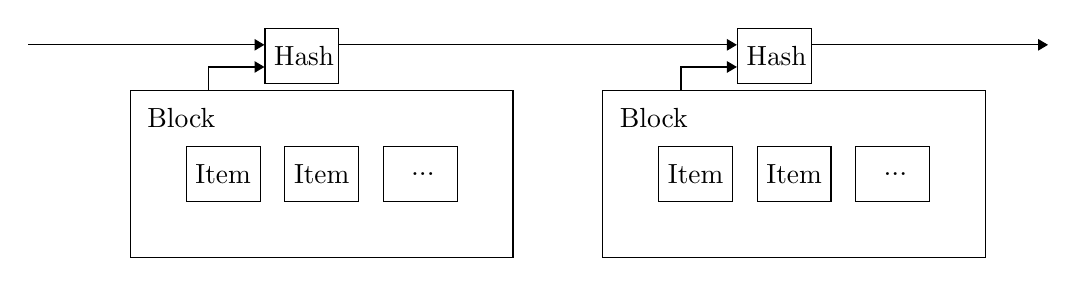
\begin{tikzpicture}[>=Triangle]
    \tikzset{box/.style={draw, minimum size=2em, text width=2em, text centered},
        container/.style={draw, inner sep=20pt}
    }

    \foreach \i / \x in {0/-2, 1/4} {
        \node (P\i-Hash) [box] at (\x, 1.5) {Hash};
        \node (Item1) [box] at (\x - 1, 0){Item};
        \node (Item2) [box] [right=0.3cm of Item1] {Item};
        \node (Item3) [box] [right=0.3cm of Item2] {...};
        \node (Container) [container] [label={[shift={(8ex,-4ex)}]north west:Block}, fit=(Item1)(Item2)(Item3)] {};

        \draw [->] (Container.north west)+(1, 0) |- ([yshift=-4]P\i-Hash.west);
    }

    \draw [<-] ([yshift=4]P0-Hash.west) --+ (-3, 0);
    \draw [->] ([yshift=4]P0-Hash.east) -- ([yshift=4]P1-Hash.west);
    \draw [->] ([yshift=4]P1-Hash.east) --+ (3, 0);
    \end{tikzpicture}
    \caption{
        The abstract concept of the distributed timestamp server. 
        Diagram recreated based on \citeauthor{nakamoto_bitcoin_2008}~\cite{nakamoto_bitcoin_2008}.
    }
    \label{fig:timechain}
\end{figure}

To secure this timechain against tampering, Bitcoin employs a Proof-of-Work consensus mechanism. 
As detailed in \autoref{fig:proof-of-work}, miners must expend computational energy in the physical world 
to find a valid \code{hash} that satisfies the network's difficulty target. 
Once a valid block is mined and appended to this chain of blocks, hence blockchain, the transactions within it are considered 
confirmed\footnote{Because blockchain reorganizations (\term{reorgs}) can occasionally occur due to network latency, 
\citeauthor{nakamoto_bitcoin_2008} mathematically showed that waiting for a transaction to be six blocks 
deep provides probabilistic finality~\cite[Section~11]{nakamoto_bitcoin_2008}.}.

\begin{figure}[htpb]
    \centering
    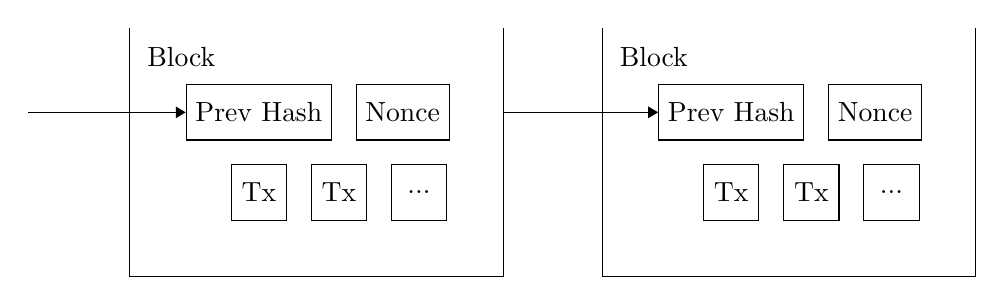
\begin{tikzpicture}[>=Triangle]
    \tikzset{box/.style={draw, minimum size=2em, text centered},
        container/.style={inner sep=20pt}
    }

    \foreach \i / \x in {0/-3, 1/3} {
        \node (P\i-PrevHash) [box] at (\x, 1) {Prev Hash};
        \node (Nonce) [box] [right=0.3cm of P\i-PrevHash] {Nonce};
        \node (Tx1) [box] [below=0.3cm of P\i-PrevHash]{Tx};
        \node (Tx2) [box] [right=0.3cm of Tx1] {Tx};
        \node (Tx3) [box] [right=0.3cm of Tx2] {...};
        \node (P\i-Container) [container] [label={[shift={(8ex,-4ex)}]north west:Block}, fit=(P\i-PrevHash)(Tx1)(Tx2)(Tx3)] {};
        \draw (P\i-Container.north west) -- (P\i-Container.south west) -- (P\i-Container.south east) -- (P\i-Container.north east);
    }

    \draw [<-] (P0-PrevHash.west) --+ (-2, 0);
    \draw [->] (P0-Container.east |- P1-PrevHash.west) -- (P1-PrevHash.west);
    \end{tikzpicture}
    \caption{
        The Proof-of-Work blockchain architecture, illustrating how transaction batches are cryptographically chained using the previous block's hash and a valid Nonce. Diagram recreated based on Nakamoto~\cite{nakamoto_bitcoin_2008}.
    }
    \label{fig:proof-of-work}
\end{figure}

Since these blocks are strictly ordered and the transactions within a block are sequentially listed, 
any confirmed output in the Bitcoin network can be deterministically located. 
This forms a three-dimensional tuple: 
the \term{block height}, the \term{transaction index} within that block, and the \term{output index} (\code{vout}) within that transaction. 
As will be detailed in later chapters, the \gls{ln} leverages this tuple,
encoded as a \code{short\_channel\_id}, to concisely identify and verify the existence of payment channels on the base layer.


\section{Scalability of Bitcoin}

By design, the Bitcoin protocol limits the size of each block to ensure that running 
a fully validating node remains computationally accessible to the public, thereby preserving network decentralization. 
Originally, a strict \qty{1}{\mega\byte} storage limit was enforced. 
As global adoption increased, this hard limit created a severe bottleneck in transaction throughput, 
leading to highly congested mempools and surging transaction fees.

These scalability challenges triggered a conflict known as the \enquote{Blocksize War}~\cite{bier_blocksize_2021}. 
A group of corporate entities and mining pools advocated for a \term{hard-fork} to increase the block size, 
while independent researchers and protocol developers argued for maintaining the limit and scaling via layered architectural upgrades. 
The developers' approach ultimately succeeded, resulting in the 2017 activation of 
a backwards-compatible soft-fork known as Segregated Witness (\term{SegWit}).

SegWit fundamentally reorganized transaction data by separating
the cryptographic signatures (the witness) from the transaction inputs. 
Most importantly for Layer-2 scalability, SegWit eliminated third-party \term{transaction malleability},
a vulnerability where an attacker could alter a \code{txid} before it was confirmed. 
By fixing this, SegWit finally made it secure to chain unconfirmed transactions together.
Furthermore, the protocol relies on \glspl{htlc}, 
which are specialized Bitcoin scripts that lock funds using hash preimages and time expirations. 
Together with the activation of SegWit, these changes laid the 
foundation for a scalable, off-chain payment network: the Lightning Network.


\section{Bitcoin Lightning Network}
\label{sec:lightning-network}

The Bitcoin Lightning Network (LN) was first proposed in 2016 by \citeauthor{poon_bitcoin_2016} 
in their whitepaper, \citetitle{poon_bitcoin_2016}~\cite{poon_bitcoin_2016}. 
Designed as a Layer-2 scaling solution, the \gls{ln} mitigates the throughput limitations
of the Bitcoin blockchain by shifting the majority of transaction volume \term{off-chain}. 
This architecture significantly conserves scarce block space while continuing
to inherit the robust, decentralized security model of the underlying network.

The fundamental building blocks of this off-chain network are \term{payment channels}. 
Technically, a payment channel is a 2-of-2 multisignature transaction, referred to as \term{funding transaction}, 
broadcasted to the Bitcoin base layer. 
Once this channel is established, the two participating nodes can exchange transactions 
by continuously signing and exchanging new \term{commitment transactions} that update the distribution of the locked funds. 
Because of SegWit, these unconfirmed state updates can be exchanged securely 
and trustlessly without requiring immediate on-chain settlement.

To make individual payment channels function as a globally routable payment network, 
nodes must follow a set of communication and cryptographic standards. 
In the following section, we elaborate on the protocol specifications, known as \glspl{bolt}. 
We specifically focus on the gossip protocol that forms the data foundation for the \tech{ln-history} platform.
We finish with an overview of the client software that implement these standards.

\section{Lightning Protocol: BOLT}
\label{sec:lightning-protocol}

The technical specifications of the \gls{ln} are formalized as the BOLTs~\cite{lightningdevelopers_lightning_2018}. 
Currently, comprising twelve documents BOLT\#1 through BOLT\#12, 
these standards ensure interoperability across different client implementations. 
Because the \tech{ln-history} platform is fundamentally designed to parse and store network topology data, 
we first introduce the protocol's core data primitives (\autoref{sec:lightning-data-model}) 
before detailing the specific gossip messages used for network discovery.


\subsection{Data Model}
\label{sec:lightning-data-model}

\subsubsection{Type-Length-Value Records (TLV)}
To ensure backwards compatibility and allow for continuous protocol upgrades, 
Lightning messages extensively utilize \gls{tlv} streams. 
Rather than relying on immutable data structures, messages append optional fields using the format illustrated in \autoref{fig:tlv_record}.

\begin{figure}[htbp]
    \centering
    \renewcommand{\arraystretch}{1.5} 
    
    \begin{tabular}{|c|c|c|}
        \hline
        % Row 1: The Field Names
        \textbf{Type} & \textbf{Length} & \textbf{Value} \\
        
        % Row 2: The Encoding / Size
        \small \textit{\gls{varint}} & \small \textit{\gls{varint}} & \small \textit{Variable ($N$ bytes)} \\
        \hline
    \end{tabular}
    \caption{
        Structure of a single TLV Record. 
        The \term{Value} field's size is determined by the integer in the \term{Length} field.
    }
    \label{fig:tlv_record}
\end{figure}

A \gls{tlv} record consists of a \term{Type} identifier and a \term{Length} indicator, 
both encoded as \gls{varint}, followed by the actual \term{Value} payload. 
Types below $2^{16}$ are reserved for official BOLT specifications, 
while higher values are available for custom or experimental application data~\cite{lightningdevelopers_lightning_2018}. 
By concatenating multiple records into a stream, nodes can safely parse known fields and 
safely ignore unrecognized types without breaking message decoding.


\subsubsection{Short Channel ID (\code{scid})}

As introduced in \autoref{sec:timechain}, 
payment channels are anchored to the Bitcoin base layer via a funding transaction. 
The \gls{scid} provides a compact, unique identifier for these channels 
by encoding their exact on-chain location into an \qty{8}{\byte} integer~\cite{lightningdevelopers_lightning_2018}.

The structure consists of the \term{block height} (\qty{3}{\byte}), 
the \term{transaction index} within that block (\qty{3}{\byte}), 
and the \term{output index} (\qty{2}{\byte}). 
For human readability, these three components are printed as decimal numbers separated by an \code{x}. 
For example, a \gls{scid} of \code{539268x845x1} indicates a channel funded in block \num{539268}, 
at transaction index \num{845}, utilizing output \num{1}\footnote{Early versions of the \gls{cln} 
implementation used a colon (\code{:}) as a separator, but this was standardized to \code{x} 
within the formal BOLT specifications~\cite{user1692333_how_2022}.}.


\subsection{Messaging: BOLT\#1}
\label{sec:lightning-message}

After introducing the core data primitives, we now examine how nodes actually communicate. 
The foundational specification is BOLT\#1 that outlines the base protocol 
for connection and data exchange within the \gls{ln}. 
Because all communication over the network is strictly encrypted and authenticated, 
the protocol formally defines a plaintext \term{Lightning Message Format} that 
emerges only after a packet is decrypted~\cite{lightningdevelopers_bolts_2018b}. 

\begin{figure}[htbp]
    \centering
    \begin{bytefield}[bitwidth=1.1em, endianness=big]{16}
        
        \bitheader{0, 15} \\
        
        %  Type (2 bytes = 16 bits) 
        \bitbox{16}{Type (2 Bytes)} \\
        
        %  Payload (Variable Length) 
        \wordbox[lrt]{1}{Payload (Variable Length)} \\
        \wordbox[lrb]{1}{\footnotesize \textit{Conforms to format matching the Type}} \\
        
        %  Extension (Variable Length / Optional) 
        \wordbox{2}{Extension (Optional TLV Stream)}
        
    \end{bytefield}
    \caption{Structure of a Lightning Message. \cite[section ~Lightning Message Format]{lightningdevelopers_lightning_2018}}
    \label{fig:lightning_message}
\end{figure}


As shown in \autoref{fig:lightning_message}, every parsed message follows to a hierarchical structure. 
The message always begins with a \qty{2}{\byte} \term{Type} field (encoded as a \gls{varint} integer),
which acts as an identifier to dictate how the subsequent variable-length \term{Payload} must be parsed. 
Finally, to ensure future protocol extensibility, messages may optionally conclude with a \gls{tlv} stream.



\subsection{P2P Node and Channel Discovery: BOLT\#7}
\label{sec:gossip-messages}

The discovery of nodes and channels which form the topology of the \gls{ln} does not rely on any third party. 
Instead, nodes use \term{(Public) Gossip Messages} which are \term{Lightning Messages} 
of type \code{256}, \code{257} or \code{258} and defined in ~\cite{lightningdevelopers_bolts_2018a}. 
The gossip protocol serves two objectives

\begin{enumerate}
    \item \textbf{Peer discovery:} 
        Every node has the properties \code{node\_id}, \code{alias}, \code{color}, 
        and a list of \code{addresses} that other nodes can use to connect to.
    \item \textbf{Channel discovery:} 
        Every node creates and maintains its own (local) view 
        of the topology of the \gls{ln}, necessary for path finding and routing.
\end{enumerate}

To fulfil these objectives, the protocol defines three distinct message types:

Firstly, the \code{channel\_announcement} (type \code{256}) establishes the topological link between two peers. 
It binds the participating nodes (\code{node\_id\_1} and \code{node\_id\_2}) to a specific on-chain \gls{scid}. 
To prevent malicious actors from spamming the network with fake topology data, 
this message requires four distinct cryptographic signatures (from both the node keys and the underlying Bitcoin funding keys). 
This guarantees that the announced channel is genuinely anchored to a confirmed Bitcoin transaction.

Secondly, the \code{node\_announcement} (type \code{257}) is broadcasted by individual nodes to declare their network reachability. 
It provides the necessary routing \code{addresses} alongside the node's metadata. 
To mitigate spam, the protocol mandates that a node may only broadcast this message 
after it has successfully verified and announced at least one public channel.

Thirdly, the \code{channel\_update} (type \code{258}) informs the network about 
the operational and economic policies of an established channel. 
Because \gls{ln} channels are bidirectional, each participating node broadcasts its own update to 
independently set the routing fees (base and proportional) and timelock requirements (\term{HTLC} minimums and maximums) 
for its specific forwarding direction. 
These updates make up the vast majority of network traffic as nodes continuously adjust their fee policies to manage their liquidity.


\subsubsection{Channel Announcement}
\label{sec:channel-announcement}

The \code{channel\_announcement} message broadcasts the existence of 
a newly established, public channel to the \gls{ln}. 
It links the founding Lightning nodes to the on-chain funding transaction that backs their channel. 
The structure of the message payload is defined by the BOLT specification and is illustrated in \autoref{fig:channel_announcement}.

\begin{figure}[htbp]
    \centering
    % 32-bit width
    \begin{bytefield}[bitwidth=1.1em, endianness=big]{32}
        \bitheader{0, 15, 16, 31} \\
        
        % Type Header 
        \wordbox{1}{\code{type} (2 bytes, value: 256)} \\

        % Signatures 
        \wordbox[lrt]{1}{4 $\times$ 64-byte signatures} \\
        \wordbox[lrb]{1}{\code{node\_sig\_1}, \code{node\_sig\_2}, \code{bitcoin\_sig\_1}, \code{bitcoin\_sig\_2}} \\
        
        % Features 
        \bitbox{16}{\code{len} (2 bytes)} & \bitbox{16}{\code{features} (\code{len} bytes)} \\
        
        % Chain Hash 
        \wordbox{1}{\code{chain\_hash} (32 bytes)} \\
        
        % SCID 
        \wordbox{2}{\code{short\_channel\_id} (8 bytes)} \\

        % Node IDs 
        \wordbox{1}{\code{node\_id\_1} (33 bytes)} \\
        \wordbox{1}{\code{node\_id\_2} (33 bytes)} \\
        
        % Bitcoin Keys
        \wordbox{1}{\code{bitcoin\_key\_1} (33 bytes)} \\
        \wordbox{1}{\code{bitcoin\_key\_2} (33 bytes)}
        
    \end{bytefield}
    \caption{
        Byte layout of the \code{channel\_announcement} message. 
        Large fields are shown as blocks~\cite[Section~channel\_announcement]{lightningdevelopers_lightning_2018}.
    }
    \label{fig:channel_announcement}
\end{figure}

The fields are defined as follows:
\begin{description}
    \item[Signatures] 
        Four \qty{64}{\byte} cryptographic signatures. 
        Together, they prove that both Lightning nodes agree on the channel and 
        that they own the associated on-chain funding outputs. 
    
    \item[\code{features}] 
        A \gls{varint} bitfield used to signal supported protocol extensions (defined in BOLT\#9~\cite{lightningdevelopers_bolts_2018}). 
        This ensures forward compatibility, allowing older nodes to process announcements from newer nodes without breaking network consensus.

    \item[\code{chain\_hash}] 
        A \qty{32}{\byte} unique identifier for the underlying blockchain, 
        represented as the hash of the chain's genesis block encoded in \gls{le} 
        format\footnote{For instance, the \code{chain\_hash} for the Bitcoin Mainnet is 
        \code{6fe28c0ab6f1b372c1a6a246ae63f74f931e8365e15a089c68d6190000000000}~\cite{lightningdevelopers_lightning_2018}.}. 
        This prevents channels established on testnets or forks from being maliciously announced on the main network.

    \item[\code{short\_channel\_id}] 
        The \qty{8}{\byte} base-layer tuple (\term{block height}, \term{transaction index}, and \term{output index}) 
        mapping exactly to the channel's funding transaction.

    \item[\code{node\_id}] 
        The \qty{33}{\byte} compressed public keys of the two participating Lightning nodes. 
        To ensure a deterministic message format and prevent peers from broadcasting duplicate announcements by swapping the fields, 
        \code{node\_id\_1} must be lexicographically strictly less than \code{node\_id\_2}.  

    \item[Bitcoin Keys] 
        The \qty{33}{\byte} compressed public keys utilized in the 2-of-2 multisignature transaction. 
        These are distinct from the Lightning \code{node\_id} keys and are required to verify the on-chain Bitcoin signatures.
\end{description}


\subsubsection{Node Announcement \code{257}}

The \code{node\_announcement} message allows a node to advertise its presence, metadata, and connectivity details to the \gls{ln}.
The protocol specifies the byte layout shown in \autoref{fig:node_announcement}.

\begin{figure}[htbp]
    \centering
    % 32-bit width
    \begin{bytefield}[bitwidth=1.1em, endianness=big]{32}
        \bitheader{0, 15, 16, 31} \\
        
        % Type 
        \wordbox{1}{\code{type} (2 bytes, value: 257)} \\
        
        % Signature 
        \wordbox{2}{\code{signature} (64 bytes)} \\
        
        % Features 
        \bitbox{16}{\code{flen} (2 bytes)} & \bitbox{16}{\code{features} (\code{flen} bytes)} \\
        
        % Timestamp 
        \wordbox{1}{\code{timestamp} (4 bytes)} \\
        
        % ID 
        \wordbox{1}{\code{node\_id} (33 bytes)} \\
        
        % Color & Alias 
        \wordbox{1}{\code{rgb\_color} (3 bytes)} \\
        \wordbox{1}{\code{alias} (32 bytes)} \\
        
        % Addresses 
        \wordbox{1}{\code{addrlen} (2 bytes)} \\
        \wordbox{1}{\code{addresses} (\code{addrlen} bytes)}
    \end{bytefield}
    \caption{
        Byte layout of the \code{node\_announcement} message. 
        Large fields are shown as blocks~\cite[Section~node\_announcement]{lightningdevelopers_lightning_2018}.
    }
    \label{fig:node_announcement}
\end{figure}

The fields are defined as follows:
\begin{description}
    \item[\code{signature}] 
        A \qty{64}{\byte} cryptographic signature over the message hash. 
        This proves that the message originated from the exact \code{node\_id} being announced, 
        preventing peers from spoofing a node's routing configuration.
    
    \item[\code{features}] 
        A \gls{varint} bitfield (dictated by \code{flen}) used to signal supported protocol extensions. 
        As with \code{channel\_announcements}, this ensures forward compatibility across the network.
    
    \item[\code{timestamp}] 
        A \qty{4}{\byte} Unix timestamp. 
        Because nodes dynamically update their network addresses and configurations, 
        this timestamp allows peers to strictly order incoming updates and safely discard stale announcements.

    \item[\code{node\_id}] 
        The \qty{33}{\byte} compressed public key that cryptographically identifies the announcing node on the \gls{ln}.
    
    \item[\code{alias} and \code{rgb\_color}] 
        Metadata allowing operators to customize their node's display name (\tech{UTF-8} encoded) and visual appearance in network explorers. 
        Because these values are entirely arbitrary and unauthenticated, they offer no security guarantees and could be used for impersonation attacks.
    
    \item[\code{addresses}] 
        A \gls{varint} field (dictated by \code{addrlen}) specifying the network transport protocols available for connection. 
        A node may advertise multiple addresses simultaneously, supporting 
        IPv4, IPv6, Tor (v2 and v3) onion services, and DNS hostnames~\cite[Section~node\_announcement]{lightningdevelopers_lightning_2018}.
\end{description}



\subsubsection{Channel Update \code{258}}

Because \gls{ln} channels are bidirectional, routing policies are managed independently for each direction. 
The direction routing from \code{node\_id\_1} to \code{node\_id\_2} is designated as direction \code{0}, 
while the reverse is designated as direction \code{1}. 
After a channel is established, each participant independently broadcasts a \code{channel\_update} message 
to specify their respective fee structure and operational limits~\cite[Section~channel\_update]{lightningdevelopers_lightning_2018}.

\begin{figure}[htbp]
    \centering
    % 32-bit width (4 bytes per row)
    \begin{bytefield}[bitwidth=1.1em, endianness=big]{32}
        
        \bitheader{0,15,16,31} \\
        
        % Type 
        \wordbox{1}{\code{type} (2 bytes, value: 258)} \\
        
        % Signature 
        \wordbox{2}{\code{signature} (64 bytes)} \\
        
        % Chain Hash 
        \wordbox{1}{\code{chain\_hash} (32 bytes)} \\
        
        % SCID (8 bytes = 2 rows) 
        \wordbox{2}{\code{short\_channel\_id} (8 bytes)} \\
        
        % Timestamp 
        \wordbox{1}{\code{timestamp} (4 bytes)} \\
        
        % Flags (1 + 1 + 2 = 4 bytes) 
        \bitbox{8}{\code{msg\_flags} (1 B)} & \bitbox{8}{\code{ch\_flags} (1 B)} & \bitbox{16}{\code{cltv\_expiry\_delta} (2 B)} \\
        
        % Values (u64 = 8 bytes = 2 rows) 
        \wordbox{2}{\code{htlc\_minimum\_msat} (8 bytes)} \\
        \wordbox{1}{\code{fee\_base\_msat} (4 bytes)} \\
        \wordbox{1}{\code{fee\_prop\_millionths} (4 bytes)} \\
        \wordbox{2}{\code{htlc\_maximum\_msat} (8 bytes)}
        
    \end{bytefield}
    \caption{
        Byte layout of the \code{channel\_update} message. 
        Large fields are shown as blocks~\cite[Section~channel\_update]{lightningdevelopers_lightning_2018}.
    }
    \label{fig:channel_update}
\end{figure}

\begin{description}
    \item[Signature] 
        One \qty{64}{\byte} signatures prove that the message has been sent by the nodes that 
        participate in the channel that the update belongs to.

    \item[Metadata] 
        Contains the \code{timestamp} to order updates, the \code{chain\_hash} indicates the correct network and 
        the \code{\gls{scid}} identifies the channel to update.

    \item[Flags] 
        Bitfields containing control information. 
        The most important is the \code{direction} bit (in \code{channel\_flags}), 
        which signals if the update applies to \code{node\_1} $\rightarrow$ \code{node\_2} or the reverse. 
        The \code{disable} bit can be used to temporarily disable the channel.
    
    \item[Fee Policy] 
        Consists of two parameters: \code{fee\_base\_msat} and \code{fee\_proportional\_millionths}. 
        A payment with an amount of $n$\,\unit{\milli\sat} needs to pay a fee following the calculation of \autoref{eq:fee_policy}.
    \begin{align}
        Fee(n) = \code{fee\_base\_msat} + \left( n \cdot \frac{\code{fee\_prop\_millionths}}{1\,000\,000} \right)
        \label{eq:fee_policy}
    \end{align}

    \item[\gls{htlc} Limits] 
        The \code{cltv\_expiry\_delta} defines the required time-lock buffer. 
        The \code{htlc\_minimum\_msat} and \code{htlc\_maximum\_msat} fields define 
        the smallest and largest payment sizes allowed to pass through this channel, respectively.
\end{description}


\subsection{Gossip Synchronization and Queries}
\label{sec:gossip-queries}

While the announcement and update messages described above contain the actual topological data of the \gls{ln}, 
nodes require a standardized mechanism to request this data. 
When a node bootstraps or reconnects after being offline, 
it must synchronize its local graph with the network to ensure its routing tables are accurate. 

To facilitate this, BOLT\#7 defines a suite of query messages that allow nodes to request 
targeted subsets of the gossip data rather than downloading 
the entire network history unnecessarily~\cite[Section~Query Messages]{lightningdevelopers_lightning_2018}.
We divide the query messages into their two-step synchronization workflow:

\begin{enumerate}
    \item \textbf{Macro-Synchronization (\code{query\_channel\_range}):} 
        A node first asks a peer for all active channels created within a specific window of Bitcoin blocks. 
        The peer responds with a \code{reply\_channel\_range} message, returning a compressed array of \glspl{scid} 
        that match the requested timeframe.
    \item \textbf{Micro-Synchronization (\code{query\_short\_channel\_ids}):} 
        Once the requesting node has the list of \glspl{scid}, it compares them against its local database. 
        For any missing or outdated channels, it sends a \code{query\_short\_channel\_ids} message 
        to explicitly request the exact \code{channel\_announcement} and \code{channel\_update} payloads for those specific channels.
\end{enumerate}


\section{Bitcoin Lightning Implementations}
\label{sec:implementations}

There are several (commercial) companies as well as organizations that have 
implemented the described specifications, each with their own technology and different focus,
but all have their codebase open-sourced.
As the following \autoref{tab:lightning-nodes-implementation} shows, there are, as of writing, 
four working implementations and one getting build.

\begin{table}[htpb]
    \centering
    \caption{Comparison of major Bitcoin Lightning Network implementations.}
    \label{tab:lightning-nodes-implementation}
    \renewcommand{\arraystretch}{1.4}
    \begin{tabular}{@{} l l l c @{}}
        \toprule
        \textbf{Implementation} & 
        \begin{tabular}{@{}l@{}}\textbf{Primary} \\ \textbf{Language}\end{tabular} & 
        \begin{tabular}{@{}l@{}}\textbf{Lead} \\ \textbf{Maintainer}\end{tabular} & 
        \textbf{Est.} \\
        \midrule
        \textbf{\gls{lnd}} & Go & Lightning Labs & 2016 \\
        \textbf{Core Lightning (CLN)} & C & Blockstream & 2015 \\
        \textbf{Eclair} & Scala & ACINQ & 2015 \\
        \textbf{\gls{ldk}} & Rust & Spiral & 2019 \\
        \textbf{NLightning} & C\# .NET & N\'{i}ckolas Goline & 2024 \\
        \bottomrule
    \end{tabular}
\end{table}

\paragraph{\gls{lnd}}
Developed by Lightning Labs in Go, \gls{lnd}~\cite{lnddeveloper_lightningnetwork_2026} 
is currently the most widely deployed node implementation on the network. 
Its design focuses on enterprise tooling, featuring a developer-friendly architecture with extensive gRPC and REST APIs.

\paragraph{\gls{cln}}
Maintained primarily by Blockstream, \gls{cln}~\cite{corelightningdevelopers_elementsproject_2026} 
is written in C and follows a UNIX-style philosophy. 
It separates distinct node functions into isolated daemons, 
making it lightweight with a flexible, multi-language plugin system.

\paragraph{Eclair}
Built by ACINQ in Scala, Eclair~\cite{eclairdevelopers_acinq_2026} 
is an enterprise-grade node engineered specifically to handle high-volume routing. 
It is optimized for native mobile integrations and serves as the backbone for 
ACINQ's Phoenix wallet, which shows its capabilities in managing asynchronous connectivity for light clients.

\paragraph{\gls{ldk}}
Unlike standalone node daemons, the \gls{ldk}~\cite{ldkdevelopers_lightningdevkit_2026}, 
managed by Spiral, is a modular, Rust-based development toolkit. 
It gives engineers a flexible API to embed custom Lightning capabilities directly 
into existing applications and wallets, removing the operational overhead of managing a full, localized routing node.

\paragraph{NLightning}
is the newest addition to the ecosystem. NLightning~\cite{goline_ngoline_2026} 
is an actively developing C\# .NET implementation of the BOLT specifications. 
It aims to provide a robust, enterprise-ready implementation designed for 
critical usage within the broader .NET developer ecosystem.


While all implementations successfully execute the BOLT specifications, 
their different architectures make them suitable for different tasks. 
For the purpose of raw gossip data collection, the \gls{cln} implementation presents many advantages. 
Its UNIX-style separation of daemons and its extensible plugin architecture allows 
hooking directly into the node's internal event streams without needing to modify any software. 
Because this design enables real-time access to raw \gls{p2p} gossip messages, 
\gls{cln} serves as the implementation of choice for the \tech{ln-history} platform's data collection.
This will be detailed in the following chapter (\autoref{ch:architecture}).





\iffalse
It is further necessary to specify the 
As soon as a transaction is incorporated into a valid Bitcoin block, meaning a miner has broadcasted a block with a valid block-hash, 
the transaction changes its previously \gls{utxo} to so-called \textit{Spent Transaction Outputs}. Each transaction output represents an amount of bitcoin.
Transactions in their "raw form" can be displayed in hex as seen in \autoref{lst:first-transaction-hex}. 
To better understand this important concept we analyse the very first bitcoin transaction (that was not a coinbase transaction) which occured in block 170 where Satoshi Nakamoto transferred $\si{10}{BTC}$ to Hal Finney.
\begin{listing}[H]
\begin{minted}[
    breaklines=true, 
    breakanywhere=true,
    frame=single, 
    bgcolor=black!5,
    fontsize=\small
]{text}
> bitcoin-cli getrawtransaction f4184fc596403b9d638783cf57adfe4c75c605f6356fbc91338530e9831e9e16

0100000001c997a5e56e104102fa209c6a852dd90660a20b2d9c352423edce25857fcd3704000000004847304402204e45e16932b8af514961a1d3a1a25fdf3f4f7732e9d624c6c61548ab5fb8cd410220181522ec8eca07de4860a4acdd12909d831cc56cbbac4622082221a8768d1d0901ffffffff0200ca9a3b00000000434104ae1a62fe09c5f51b13905f07f06b99a2f7159b2225f374cd378d71302fa28414e7aab37397f554a7df5f142c21c1b7303b8a0626f1baded5c72a704f7e6cd84cac00286bee0000000043410411db93e1dcdb8a016b49840f8c53bc1eb68a382e97b1482ecad7b148a6909a5cb2e0eaddfb84ccf9744464f82e160bfa9b8b64f9d4c03f999b8643f656b412a3ac00000000
\end{minted}
\caption{Retrieving the raw transaction data by txid via bitcoin-cli.}
\label{lst:first-transaction-hex}
\end{listing}

Following the bitcoin protocol this long string of byte data can be organized into 'standardized' fields.
There are three different types of field.
The fixed length, variable length and. 
Fixed length means that there is a pre-set number of bytes allowed for that field .
Variable Length.

The first $\si{4}{B}$ are always the version. Parsing of 01000000 needs to be done using little-endian yielding version: 1.
Next the number of inputs is one byte $01$ meaning 1.
Next $\si{32}{B}$ is the transactionID (c997a5e56e104102fa209c6a852dd90660a20b2d9c352423edce25857fcd3704) always fixed which must be parsed as little endian yielding to: 0437cd7f8525ceed2324359c2d0ba26006d92d856a9c20fa0241106ee5a597c9
This is followed by the output number which is always a fixed 8-byte: 0000000048473044 which cields to 
()

\begin{table}[htpb]
    \centering
    \caption{Hexadecimal breakdown of the first transaction from Satoshi to Hal Finney.}
    \label{tab:tx-hex-breakdown}
    \renewcommand{\arraystretch}{1.3}
    \begin{tabularx}{\textwidth}{|>{\ttfamily\footnotesize\raggedright\arraybackslash}p{3.5cm}|>{\raggedright\arraybackslash}X|l|l|}
        \hline
        \rowcolor{black!10}
        \textbf{Raw Hex Segment} & \textbf{Field Description} & \textbf{Data Type} & \textbf{Size} \\ \hline
        01000000 & \textbf{Version:} 1 & Fixed & 4 Bytes \\ \hline
        01 & \textbf{Input Count:} 1 & CompactSize & 1 Byte \\ \hline
        \multicolumn{4}{|c|}{\cellcolor{blue!10}\textbf{Input 0 (from previous Satoshi transaction)}} \\ \hline
        c997a5e5...7fcd3704 & \textbf{Previous TXID:} (Internal little-endian order) & Fixed & 32 Bytes \\ \hline
        00000000 & \textbf{Previous Output Index:} 0 & Fixed & 4 Bytes \\ \hline
        48 & \textbf{Script Length:} 72 Bytes & CompactSize & 1 Byte \\ \hline
        47304402...1d0901 & \textbf{ScriptSig:} Unlocking script (Signature) & Variable & 72 Bytes \\ \hline
        ffffffff & \textbf{Sequence:} Standard final sequence & Fixed & 4 Bytes \\ \hline
        02 & \textbf{Output Count:} 2 & CompactSize & 1 Byte \\ \hline
        \multicolumn{4}{|c|}{\cellcolor{green!10}\textbf{Output 0 (10 BTC Transferred to Hal Finney)}} \\ \hline
        00ca9a3b00000000 & \textbf{Amount:} $10 \text{ BTC} = 10^9 \text{ sats}$ ($3b9aca00_{16}$) & Fixed & 8 Bytes \\ \hline
        43 & \textbf{Script Length:} 67 Bytes & CompactSize & 1 Byte \\ \hline
        4104ae1a...d84cac & \textbf{ScriptPubKey:} P2PK Locking script & Variable & 67 Bytes \\ \hline
        \multicolumn{4}{|c|}{\cellcolor{red!10}\textbf{Output 1 (40 BTC Change returned to Satoshi)}} \\ \hline
        00286bee00000000 & \textbf{Amount:} $40 \text{ BTC} = 4 \times 10^9 \text{ sats}$ ($ee6b2800_{16}$) & Fixed & 8 Bytes \\ \hline
        43 & \textbf{Script Length:} 67 Bytes & CompactSize & 1 Byte \\ \hline
        410411db...12a3ac & \textbf{ScriptPubKey:} P2PK Locking script & Variable & 67 Bytes \\ \hline
        00000000 & \textbf{Locktime:} 0 & Fixed & 4 Bytes \\ \hline
    \end{tabularx}
\end{table}


\subsubsection{Query and Reply Messages}

A node needs to request its peers to receive new gossip messages. Likewise a peer needs to respond to those \term{Query Messages} using their adequate reply. In \code{BOLT 07} there are three \term{request} and two \term{reply messages} specified and shown in \autoref{tab:gossip-query-reply-bolt-07}.

\begin{table}[htbp]
    \centering
    
    % Define 4 columns: Request Type, Request Name, Reply Type, Reply Name
    \begin{tabular}{@{} ll ll @{}}
        \toprule
        \multicolumn{2}{c}{\textbf{Request}} & \multicolumn{2}{c}{\textbf{Reply}} \\
        \cmidrule(r){1-2} \cmidrule(l){3-4} 
        \textbf{Type} & \textbf{Name} & \textbf{Type} & \textbf{Name} \\
        \midrule
        
        \code{261} & \code{query\_short\_channel\_ids} & \code{262} & \code{reply\_short\_channel\_ids\_end} \\
        \code{263} & \code{request\_channel\_range}    & \code{264} & \code{reply\_channel\_range} \\
        \code{265} & \code{gossip\_timestamp\_filter}  &           & --- \\
        
        \bottomrule
    \end{tabular}

    \caption{Gossip query and reply message types defined in BOLT 07. Note that \code{gossip\_timestamp\_filter} does not trigger a direct reply~\cite[section ~Query Messages]{lightningdevelopers_lightning_2018}.}
    \label{tab:gossip-query-reply-bolt-07}
    
\end{table}

\paragraph{Query Short Channel Ids \code{261}}
~\cite[section ~query\_short\_channel\_ids]{lightningdevelopers_lightning_2018}
\begin{figure}[htbp]
    \centering
    % 32-bit width (4 bytes per row)
    \begin{bytefield}[
        bitwidth=1.1em, endianness=big]{32}
        \bitheader{0,15,16,31} \\
        
        % --- Type ---
        \bitbox{16}{\code{type} (261)} & \bitbox{16}{} \\
        
        % --- Chain Hash (32 bytes) ---
        \wordbox{1}{\code{chain\_hash} (32 bytes)} \\
        
        % --- Len (u16) + Padding for visual alignment ---
        % 'len' is 2 bytes. We place it on the left.
        \bitbox{16}{\code{len} (u16)} & \bitbox{16}{\textit{(reserved space)}} \\
        
        % --- Encoded Short IDs (Variable Length) ---
        % The length is determined by 'len' above
        \wordbox[lrt]{1}{\code{encoded\_short\_ids}} \\
        \wordbox[lrb]{1}{(\code{len} bytes)} \\
        
        % --- TLVs (Variable Stream) ---
        % Contains query_flags (type 1)
        \wordbox[lrt]{1}{\code{tlvs}} \\
        \wordbox[lrb]{1}{(variable length stream)} \\
        
    \end{bytefield}
    \caption{Byte layout of the \code{query\_short\_channel\_ids} message. The \code{encoded\_short\_ids} field contains compressed \gls{scid}s, and the \code{tlvs} field may contain \code{query\_flags} to filter the response~\cite[section ~query\_short\_channel\_ids]{lightningdevelopers_lightning_2018}.}
    \label{fig:query_short_channel_ids}
\end{figure}


\paragraph{Reply Short Channel Ids End \code{262}}

\begin{figure}[htbp]
    \centering
    % 32-bit width (4 bytes per row)
    \begin{bytefield}[
        bitwidth=1.1em, endianness=big]{32}
        \bitheader{0,15,16,31} \\
        
        % --- Type (2 bytes) ---
        \bitbox{16}{\code{type} (262)} & \bitbox{16}{} \\
        
        % --- Chain Hash (32 bytes) ---
        \wordbox{1}{\code{chain\_hash} (32 bytes)} \\
        
        % --- Full Information (1 byte) ---
        % We explicitly show the 1 byte and leave 3 bytes empty for alignment.
        \bitbox{8}{\code{full\_info}} & \bitbox{24}{} \\
        
    \end{bytefield}
    \caption{Byte layout of the \code{reply\_short\_channel\_ids\_end} message. The \code{full\_information} byte (previously named \code{complete}) signals if the replying node believes it has provided all available data~\cite[section ~reply\_short\_channel\_ids\_end]{lightningdevelopers_lightning_2018}.}
    \label{fig:reply_short_channel_ids_end}
\end{figure}


\paragraph{Request Channel Range \code{263}}
\begin{figure}[htbp]
    \centering
    % 32-bit width (4 bytes per row)
    \begin{bytefield}[
        bitwidth=1.1em, endianness=big]{32}
        \bitheader{0,15,16,31} \\
        
        % --- Type ---
        \bitbox{16}{\code{type} (263)} & \bitbox{16}{} \\
        
        % --- Chain Hash ---
        \wordbox{1}{\code{chain\_hash} (32 bytes)} \\
        
        % --- First Blocknum (u32) ---
        \bitbox{32}{\code{first\_blocknum} (u32)} \\
        
        % --- Number of Blocks (u32) ---
        \bitbox{32}{\code{number\_of\_blocks} (u32)} \\
        
        % --- TLVs (Variable) ---
        % Contains query_option (type 1)
        \wordbox[lrt]{1}{\code{tlvs}} \\
        \wordbox[lrb]{1}{(variable stream)} \\
        
    \end{bytefield}
    \caption{Byte layout of the \code{query\_channel\_range} message. The \code{tlvs} field may contain \code{query\_option} flags to request timestamps or checksums for the specified block range~\cite[section ~query\_channel\_range]{lightningdevelopers_lightning_2018}.}
    \label{fig:query_channel_range}
\end{figure}


\paragraph{Reply Chanel Range \code{264}}

\begin{figure}[htbp]
    \centering
    % 32-bit width (4 bytes per row)
    \begin{bytefield}[
        bitwidth=1.1em, endianness=big]{32}
        \bitheader{0,15,16,31} \\
        
        % --- Type ---
        \bitbox{16}{\code{type} (264)} & \bitbox{16}{} \\
        
        % --- Chain Hash ---
        \wordbox{1}{\code{chain\_hash} (32 bytes)} \\
        
        % --- Block Ranges ---
        \bitbox{32}{\code{first\_blocknum} (u32)} \\
        \bitbox{32}{\code{number\_of\_blocks} (u32)} \\
        
        % --- Sync Complete (1 byte) & Len (2 bytes) ---
        % Total 24 bits used. We leave 8 bits empty for visual alignment 
        % before starting the large data blocks.
        \bitbox{8}{\code{sync}} & 
        \bitbox{16}{\code{len} (u16)} & 
        \bitbox{8}{} \\
        
        % --- Encoded Short IDs ---
        \wordbox[lrt]{1}{\code{encoded\_short\_ids}} \\
        \wordbox[lrb]{1}{(\code{len} bytes)} \\
        
        % --- TLVs ---
        % May contain timestamps (type 1) and checksums (type 3)
        \wordbox[lrt]{1}{\code{tlvs}} \\
        \wordbox[lrb]{1}{(timestamps / checksums)} \\
        
    \end{bytefield}
    \caption{Byte layout of the \code{reply\_channel\_range} message. The \code{sync} (\code{sync\_complete}) byte indicates if this is the final reply in a sequence. The \code{tlvs} stream may contain \code{encoded\_timestamps} and \code{checksums} to facilitate efficient reconciliation~\cite[section ~reply\_channel\_range]{lightningdevelopers_lightning_2018}.}
    \label{fig:reply_channel_range}
\end{figure}


\paragraph{Gossip Timestamp Filter \code{265}}
\begin{figure}[htbp]
    \centering
    % 32-bit width (4 bytes per row)
    \begin{bytefield}[
        bitwidth=1.1em, endianness=big]{32}
        \bitheader{0,15,16,31} \\
        
        % --- Type ---
        \bitbox{16}{\code{type} (265)} & \bitbox{16}{} \\
        
        % --- Chain Hash ---
        \wordbox{1}{\code{chain\_hash} (32 bytes)} \\
        
        % --- First Timestamp (u32) ---
        \bitbox{32}{\code{first\_timestamp} (u32)} \\
        
        % --- Timestamp Range (u32) ---
        \bitbox{32}{\code{timestamp\_range} (u32)} \\
        
    \end{bytefield}
    \caption{Byte layout of the \code{gossip\_timestamp\_filter} message. This message constrains relayed gossip to a specific time window defined by \code{first\_timestamp} and the duration \code{timestamp\_range}~\cite[section ~gossip\_timestamp\_filter]{lightningdevelopers_lightning_2018}.}
    \label{fig:gossip_timestamp_filter}
\end{figure}

\fi
    \chapter{Architecture}
\label{ch:architecture}

This chapter presents the architectural design and implementation of the \tech{ln-history} platform. 
Building upon the fundamental concepts of the \gls{ln} and its gossip protocol, 
we first define the system requirements in \autoref{sec:requirements} 
followed by an architectural overview in \autoref{sec:high-level-architecture}.
After that the structure of this chapter mirrors the data flow within the system.
We begin by analysing each component sequentially, 
from different ingestion pipelines presented in \autoref{sec:real-time-pipeline} for
real-time analysis and \autoref{sec:batch-pipeline} for bulk insertion. 
To the storage layer in \autoref{sec:database} and its two auxiliary services:
Metadata enrichment in \autoref{sec:chain-enricher} and node behaviour monitoring \autoref{sec:peer-manager}.
After that the backend \service{ln-history-api} is explained in \autoref{sec:ln-history-api}.
To work with the results, we introduce a custom client library in \autoref{sec:ln-history-python-client}
The chapter comes to an end by first discusses continuous monitoring of the system in \autoref{sec:observability}.
Ultimately, the \autoref{sec:deployment} focuses on deployment.
As architecture decisions are often based on \textit{trade-offs} some sections
conclude with a discussion about their particular design decisions. 


\section{Requirements}
\label{sec:requirements}

The status quo of (public) datasets containing gossip of the \gls{ln} is a fragmented collection
of files and repositories hosted by various researchers (see \autoref{ch:related-work}). 
These datasets lack a unified structure, varying in their serialization formats 
(e.g., raw hex-encoded dumps versus pre-parsed JSON files) and metadata quality.

The current benchmarking tool for parsing these messages is the \term{time-machine},
developed by \citeauthor{decker_lnresearch_2020}~\cite{decker_lnresearch_2020}.
The \term{time-machine} tool iterates through a file of gossip messages encoded in hex and yields a \tech{networkx} graph~\cite{hagberg_exploring_2008}.
This, simple yet, effective procedure takes around 10 minutes on commodity hardware (e.g., Apple M1, 16 GB RAM) 
to process ten million gossip messages and yields a single graph for a single timestamp.
Creating $n$ snapshots requires $n$ iterations of the \term{time-machine} tool
through every collected gossip message resulting in redundant computation.  

Further, gossip data analysis (e.g. gossip propagation lag) also needs a whole iteration through the file of gossip messages
due to the fact that no index or meta information exists for a single gossip message.

To address these limitations, the \term{ln-history} platform is designed to 
transition from linear file processing to a database-centric architecture,
indexing gossip messages and reducing the workload for various analytical queries
e.g. snapshot generation from $\mathcal{O}(n)$ to $\mathcal{O}(\log n)$ or even $\mathcal(1)$. 

The system must fulfil the following functional and non-functional requirements, 
categorized by their operational scope.

\subsection{Functional Requirements}

The requirements are divided into data storage, analysis, and real-time capability. 
Each requirement has a label which will be referenced when being taken into account in the architectural design.

\subsubsection{Data Storage \& Persistence}
\begin{enumerate}[label=\textbf{RF\arabic*}, ref=RF\arabic*, leftmargin=3.5em]
    \item \label{req:dual-format} \textbf{Dual-Format Persistence:} 
        All gossip messages must be stored in both their raw wire format (bytes) for 
        bandwidth-efficient retrieval and a parsed format (structured data) for in-depth analytical querying.
    \item \label{req:persistance} \textbf{Long-Term Persistence:} 
        The system must ensure durable storage of all collected messages, serving as a permanent archive of the \gls{ln} history.
\end{enumerate}

\subsubsection{Querying \& Historic Analysis}
\begin{enumerate}[label=\textbf{RF\arabic*}, ref=RF\arabic*, resume, leftmargin=3.5em]
    \item \label{req:snapshot} \textbf{Snapshot Retrieval:} 
        The system must return the precise set of gossip messages 
        that make up the valid network state at any given timestamp.
    \item \label{req:snapshot-diff} \textbf{Time-Window Retrieval:} 
        The system must support range queries to retrieve all messages 
        broadcast between two given timestamps $t_{start}$ and $t_{end}$.
    \item \label{req:entity-filtering} \textbf{Entity Filtering:} 
        The system must be able to filter gossip history by specific identifiers, specifically \code{node\_id} and \code{scid}.
\end{enumerate}

\subsubsection{Real-Time Operations}
\begin{enumerate}[label=\textbf{RF\arabic*}, ref=RF\arabic*, resume, leftmargin=3.5em]
    \item \label{req:ingestion} \textbf{Low-Latency Ingestion:} 
        Newly received gossip from the \gls{p2p} network must be inserted into the storage engine 
        immediately to ensure the database reflects the live state.
    \item \label{req:concurrency} \textbf{Concurrency:} 
        The system must support simultaneous operations; historic analysis queries (\gls{olap}) 
        must not block or significantly degrade the performance of real-time write operations (\gls{oltp}).
    \item \label{req:multiple-nodes} \textbf{Multiple nodes:} 
        The system must be scalable to multiple collecting nodes that feed 
        new gossip messages in parallel into the platform.
    \item \label{req:metadata}\textbf{Metadata:} 
        In addition to the gossip message itself, metadata (e.g. the collection timestamp) 
        must be linked to and stored.
    \item \label{req:batch-ingestion} \textbf{Batch Ingestion:} 
        The system must be able to insert historic messages in large batches.
\end{enumerate}


\subsection{Non-Functional Requirements}
The design is further constrained by quality attributes essential for a research tool in the Bitcoin development community.

\begin{enumerate}[label=\textbf{RN\arabic*}, ref=RN\arabic*, leftmargin=3.5em]
    \item \label{req:open-source} \textbf{Transparency \& Auditability (Open Source):} 
    Aligned with the Bitcoin ethos of \enquote{Don't trust. Verify.}, 
    the platform's source code must be fully open-source under the MIT License~\cite{opensourceinitiative_mit_1988}. 
    This ensures that the data collection methodology is transparent and 
    that results generated by the platform are scientifically reproducible by independent third parties.
    
    \item \label{req:docker} \textbf{Deployability (Containerization):} 
    To facilitate easy adoption and reproducibility, the system must be fully containerized using Docker~\cite{merkel_docker_2014}. 
    This ensures the platform is environment-agnostic, allowing it to run consistently on a developer's laptop, a university server, 
    or a cloud cluster with the potential for future orchestration via Kubernetes ~\cite{burns_borg_2016}.
    
    \item \label{req:self-host} \textbf{Efficiency (Self-Hostability):} 
    The architecture must be resource-efficient enough to run on consumer-grade hardware. 
    By lowering the barrier to entry for hosting everyone should have the opportunity to run \tech{ln-history}.

    \item \label{req:maintainability} \textbf{Maintainability:}
    The system and the underlying code must be structured to support the ongoing development. 
\end{enumerate}



\section{The Big Picture: High-Level Architecture}
\label{sec:high-level-architecture}

\citeauthor{kleppmann_designing_2017} presents the \term{Lambda Architecture} in \citetitle{kleppmann_designing_2017}
as a pattern for unifying real-time and historical data processing. 

He defines the core concept as follows:
\begin{quote}
The core idea of the lambda architecture is that incoming data should be recorded by appending immutable events to an always-growing dataset,
similarly to event sourcing. [...] The lambda architecture proposes running two different systems in parallel: 
a batch processing system [...] and a separate stream-processing system.~\cite[p.~519]{kleppmann_designing_2017}   
\end{quote}

The architecture of \tech{ln-history} implements a variation of this pattern. 
Real-time gossip messages from \gls{cln} nodes are ingested immediately while the system
simultaneously supports bulk insertion of historic gossip messages.

As the batch insertion of historic gossip messages rarely occurs, 
this process is done via a \term{backfill} script manually.
On the other hand the real-time ingestion pipeline is managed by a service called \service{gossip-processor}.

Gossip messages are stored in one central database: \service{ln-history-database}.

The \autoref{fig:architecture-high-level} illustrates the architectural design of the \tech{ln-history} platform
including both data ingestion streams: batch insertion and real-time insertion.
\begin{figure}[htbp]
    \centering
    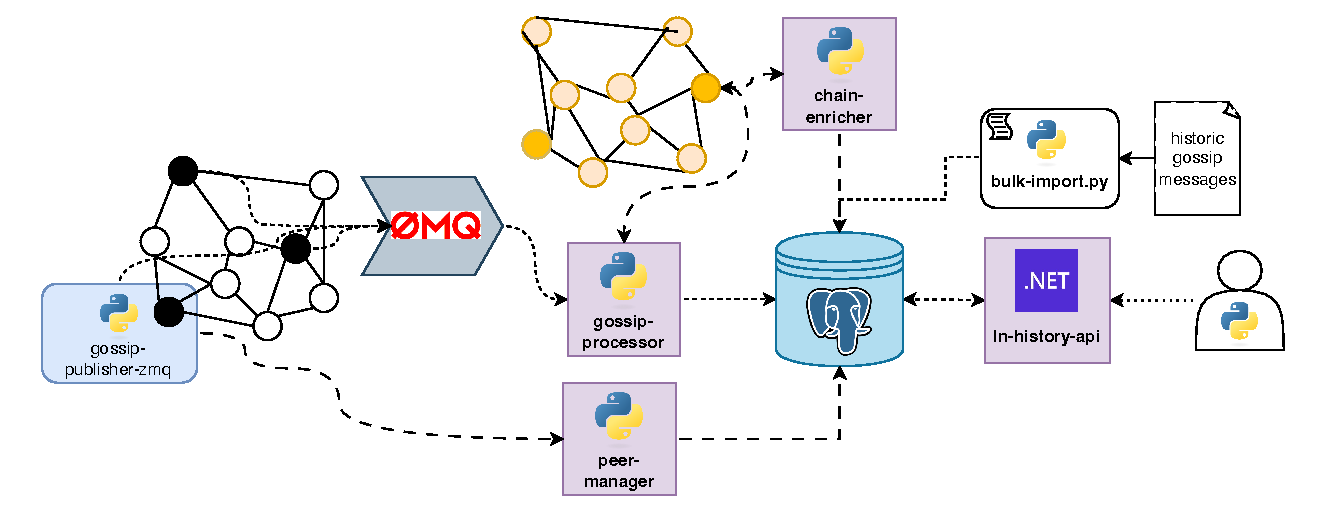
\includegraphics[width=\linewidth]{resources/images/architecture-minimal.pdf}
    \caption{High-level architecture of the \tech{ln-history} platform.}
    \label{fig:architecture-high-level}
\end{figure}

\autoref{fig:architecture-high-level} starts on the left with one or multiple 
\gls{cln} nodes indicated as filled circles which are connected to the \gls{ln} 
and run the \service{gossip-publisher-zmq} plugin.
The plugin reads the \file{gossip\_store} file and publishes new gossip messages 
enriched with additional metadata via a message queue (\tech{ZeroMQ}~\cite{hintjens_zeromq_2013}) 
to the \service{gossip\_processor} service which is indicated in purple.

The \service{gossip-processor} performs deduplication before inserting the unique 
gossip messages into the \service{ln-history-database} (coloured in blue).
Parallel to this, the \service{peer-manager} (indicated in purple) monitors every
\gls{p2p} connection for each \gls{cln} node and stores session data 
(e.g. \code{node\_id} of connected peers, session duration) into the \service{ln-history-database}.

Since the gossip messages, specifically the \code{channel\_announcement}, reference transactions 
in the Bitcoin blockchain (network is indicated in orange), 
metadata like the \code{funding\_timestamp} and \code{capacity\_sat} get retrieved externally. 
This is handled by the \service{chain-enricher} service (coloured in purple), 
which monitors the \service{ln-history-database} for those missing values.
The service extracts the \code{timestamp}\footnote{
    A block's \code{timestamp} does not necessarily represent its exact discovery time. 
    Under Bitcoin consensus rules, a timestamp is valid as long as it is strictly greater than the median 
    of the previous 11 blocks and no more than two hours ahead of the network time~\cite{bitcoincoredevelopers_bitcoin_2026a}.
} 
from the block that mined the funding transaction. It then waits for the channel
to reach the required maturity before fully enriching the database\footnote{
    A Lightning channel is not instantly valid for public routing as soon as the funding block is found. 
    According to the BOLT 7 specification, nodes must wait until the funding transaction achieves 
    at least six confirmations before broadcasting a \code{channel\_announcement}~\cite{lightningdevelopers_bolts_2018}.
}.

Lastely the \service{ln-history-api} queries the \tech{ln-history-database} 
and provides a \term{restful} API for in-depth analysis as well as secure authentication\footnote{
The \textit{SwaggerUI} shows the endpoints \url{https://api.ln-history.info/swagger/index.html}}.

On the right-hand side clients (users) request the \service{ln-history-api}. 
The \service{ln-history-python-client} provides the functionality to easily parse the response into readable formats.
To minimize bandwidth, large results like a snapshot, are sent in raw bytes following the format of \gls{ln} gossip messages.
The \service{ln-history-python-client} parses the raw bytes and returns a graph object useful for further analysis.
Additional functions to work with the \service{ln-history-api} are provided.



\section{Real-Time Ingestion Pipeline}
\label{sec:real-time-pipeline}

As described by \citeauthor{hohpe_enterprise_2012} in \citetitle{hohpe_enterprise_2012} 
the \term{Pipes and Filters} architectural style should be used to
\enquote{divide a larger processing task into a sequence of smaller independent processing steps (filters)
 that are connected by channels (pipes)}~\cite[p.~70]{hohpe_enterprise_2012}.

Adopting this pattern, the \service{gossip-publisher-zmq} plugin acts as the initial filter, 
validating the authenticity of incoming gossip messages at the \gls{cln} node level. 
Validated messages are then transmitted via a \tech{ZeroMQ} message queue to the \service{gossip-processor} service. 
The downstream component performs deduplication before persisting into the \service{ln-history-database}.

\subsection{\service{Gossip-Publisher-Zmq}}
The \service{gossip-publisher-zmq} plugin serves as the starting point for the pipeline. 
It is written in \tech{Python}~\cite{pythonsoftwarefoundation_python_2025} and 
the source code is available at~\cite{kraus_gossippublisherzmq_2026},
aligning with the requirement for open-source transparency (\ref{req:open-source}).
The plugin interfaces directly with the \gls{cln} architecture, following the 
official plugin documentation~\cite{corelightningdevelopers_cln_2026}.

\subsubsection{Data Source: The Gossip Store}
The \gls{cln} architecture delegates gossip management to the \term{gossipd deamon}. 
This process persists all gossip into a specialized append-only log file known as the \file{gossip\_store}. 
Every collected message is stored as a \term{record}, encapsulating the raw gossip payload within a structural wrapper.

The file begins with a \qty{1}{\byte} \term{File Header}. 
The top \qty{3}{\bit} encode the major version (currently \num{0}), 
while the lower \qty{5}{\bit} encode the minor version (currently \num{15}). 
Following this header, the file consists of a sequence of records. 

\begin{figure}[htbp]
    \centering
    \begin{bytefield}[bitwidth=0.8em, endianness=big]{32}
        \bitheader{0, 15, 16, 31} \\
        
        \begin{rightwordgroup}{Record Header\\(\qty{12}{\byte})}
            \bitbox{16}{\code{flags} (be16)} &
            \bitbox{16}{\code{len} ($L$) (be16)} \\
            \bitbox{32}{\code{crc} (be32)} \\
            \bitbox{32}{\code{timestamp} (be32)}
        \end{rightwordgroup} \\
        
        \begin{rightwordgroup}{Message Body\\($L$ bytes)}
            \bitbox{16}{\code{type} (be16)} &
            \bitbox[lrt]{16}{Start of Gossip Data \dots} \\
            \skippedwords \\
            \bitbox[lrb]{32}{...End of Data ($L-2$ bytes)}
        \end{rightwordgroup}
    \end{bytefield}
    \caption{Byte layout of a single record within the \gls{cln} \file{gossip\_store} file. 
            The record consists of a \qty{12}{\byte} internal header followed by the variable-length Lightning message payload. 
            All multibyte integers are stored in \gls{be} format~\cite{corelightningdevelopers_cln_2026}.}
    \label{fig:core-lightning-gossip-store-bytefield}
\end{figure}

The byte layout of an individual record is depicted in \autoref{fig:core-lightning-gossip-store-bytefield}.

\subsubsection{Retrieval Logic}
To monitor the network in real-time, the plugin opens a read-only binary handle to the 
\file{gossip\_store} file and maintains a pointer to the current file offset.

When new data is appended by the \term{gossipd daemon}, the plugin advances the file handle to read the \code{record.header}. 
It extracts the payload length ($L$) from the \code{len} field (a fixed \code{be16} integer). 
It then reads the subsequent $L$ bytes to retrieve the full message body.
Before processing, the system computes the \gls{crc32} checksum of the payload and 
compares it against the \code{record.header.crc} field to ensure data integrity.

\subsubsection{Serialization and Transmission}
After successful validation, the raw message is parsed and wrapped into a structured dictionary.

\begin{listing}[htbp]
    \begin{minted}[frame=lines, fontsize=\footnotesize]{python}
    class PluginEventMetadata(TypedDict):
        type: int
        name: str
        timestamp: int
        sender_node_id: str
        length: int  # Length in bytes without starting 2-byte type

    # Base structure for all events
    class BasePluginEvent(TypedDict):
        metadata: PluginEventMetadata
        raw_hex: str
    \end{minted}
    \caption{
        Python \code{TypedDict} definitions used as a wrapper for gossip events 
        by the \service{ln-history-python-client}~\cite{kraus_lnhistorypythonclient_2026}.
    }
    \label{lst:python-dto}
\end{listing}

\autoref{lst:python-dto} shows the \gls{dto} used in the \tech{ln-history} platform.
Metadata like the \code{sender\_node\_id} which can be set via environment variables (defaults to its own \code{node\_id}),
the \code{timestamp} when the \term{gossipd deamon} collected the message
and the length (not accounting for the \qty{2}{B} type header) of the raw message
get added to the beginning of the payload.

Finally, the structured event is broadcasted via the \tech{ZeroMQ} message queue. 
On Startup the plugin initializes a \term{PUB socket} using the host and port defined in the environment variables 
making asynchronous consumption by downstream consumers (e.g. \service{gossip-processor}) possible.


\subsection{\service{Gossip Processor}}
The \service{gossip-processor} is written in \tech{Python} and the source code can be found at ~\cite{kraus_gossipprocessor_2026}. 
It acts as a \term{SUB node}, connecting to one or more \tech{ZeroMQ} \term{PUB sockets} to consume the plugin events.
The plugin events get analysed and added into the \service{ln-history-database}.


\subsubsection{Real-time ingestion}
By utilizing a concurrent architecture, the \service{gossip-processor} can consume gossip messages 
from the network without blocking database write operations, ensuring low-latency ingestion (\ref{req:ingestion}).

The database worker continuously dequeues messages, aggregating them into batches of a configurable size 
(governed by the \code{BATCH\_SIZE} environment variable, which defaults to $200$).
Each batch is encapsulated within a single atomic transaction, ensuring data integrity in the event of a failure.

Message processing begins by storing the observation metadata (\ref{req:metadata}). 
The \code{gossip\_id}, \code{collector\_node\_id}, and the \code{seen\_at} 
timestamp are inserted into the \code{gossip\_observations} table 
tracking exactly when and by which collector node the message was seen, 
seamlessly allowing the system to scale to multiple collecting nodes (\ref{req:multiple-nodes}).

As a next step the gossip message gets upserted (create a new row or update if it exists) into the \code{gossip\_inventory} table.
If the \code{gossip\_id} is already present in the table, the query yields a \code{rowcount} of $0$, 
meaning that the gossip message is a duplicate and does not need to be further processed.

The processing branches depending on the specific gossip message type:

\paragraph{Channel Announcements}
For each \code{channel\_announcement} the \service{gossip-processor} checks foreign key constraints 
by ensuring both participating \code{node\_id}s exist in the \code{nodes} table, inserting them if they are missing.
After that, the channel is inserted into the \code{channels} table. 
While the raw message data is persisted alongside the parsed attributes, fulfilling the dual-format requirement (\ref{req:dual-format}), 
attributes derived from the underlying Bitcoin funding transaction (\code{capacity\_sat} and \code{funding\_timestamp})
are not part of BOLT\#7 messages (as discussed in \autoref{sec:gossip-messages}),
these fields are temporarily left null and are populated asynchronously by the \service{chain-enricher}.

\paragraph{Node Announcement}
Every \code{node\_announcement} messages, contains information about the sending node.
This node is upserted into the \code{nodes} table, 
updating the \code{last\_seen} timestamp upon conflict.
Since only one \code{node\_announcement} message is valid at a given timestamp, 
each message gets \code{valid\_from} and \code{valid\_to} boundaries.
When a new announcement supersedes an older one, 
the previous record's \code{valid\_to} timestamp is closed.
Due to the asynchronous nature of \gls{p2p} networks, messages can arrive out of order. 
If the \code{node\_announcement} message has a \code{timestamp} older than that of the latest,
the \service{gossip-processor} identifies it as historical data and queries the \service{ln-history-database}
to find the appropriate gap and limit the message's \code{valid\_to} boundary.

\paragraph{Channel Update}
Because \code{channel\_updates} also require temporal boundaries, 
they are processed using the same logic as \code{node\_announcements}. 
Additionally, the \service{gossip-processor} must be capable of handling \term{orphan} updates. 
These are \code{channel\_update} messages that reference a channel not (yet) registered in the \code{channels} table. 
Since a \code{channel\_update} does not contain the public keys of the participating nodes, 
it is impossible to deduce the network topology and automatically create a placeholder channel. 
Therefore, once fundamental constraints (such as the \code{gossip\_id}) are satisfied, 
the message is persisted in the \code{channel\_updates} table, but the relational 
link to a specific channel via the \code{scid} remains unestablished.

\subsubsection{Discussing Throughput Performance}

As stated in \citetitle{kleppmann_designing_2017} thinking about performance and scaling should not be the first objective.
He advocates to focus on getting things working first.~\cite[Chapter~1]{kleppmann_designing_2017}

Following this principle the initial design processed one gossip message at a time.
This approach simplified the insertion logic massively, 
but it generated an unsustainable volume of read and write operations against the \service{ln-history-database}.
Depending on the specific message type, processing a single gossip message required between three and six individual database queries.
During peak network activity, where the volume reaches an order of magnitude of $100$ gossip messages per second, 
this sequential approach exhausted the database's capacity due to high random disk I/O.

The operation of only two collector nodes already induced a cumulative processing lag 
and made the database throughput the primary bottleneck for scalability \tech{ln-history}.

To resolve this limitation, the ingestion pipeline was refactored to aggregate gossip messages into batches,
that are executed within a single atomic database transaction.

This architectural upgrade reduced the transaction overhead and the frequency of disk writes, 
yielding improvements in the overall throughput and enabling scaling.


\section{The Batch Ingestion Pipeline}
\label{sec:batch-pipeline}
The batch ingestion pipeline is done via a \tech{Python} script called \file{bulk-import.py} 
and the source code found at\footnote{\url{https://ln-history.info/bulk-import.py}}.

Because historic imports are rare, high-volume operations applied to bounded datasets, 
a dedicated batch processing script is utilized to fulfil the batch ingestion requirement (\ref{req:batch-ingestion}).
As outlined by \citeauthor{kleppmann_designing_2017}~\cite{kleppmann_designing_2017}, 
batch processing frameworks maximize throughput by avoiding random, individual database writes. 

Unlike the real-time \service{gossip-processor}, which relies on the database for conflict resolution, 
this script optimizes performance by performing data grouping and temporal boundary calculations 
entirely in memory prior to executing bulk database inserts. It achieves this using a two-pass algorithm.


\paragraph{Step 1: Parsing and Aggregation}
In the first pass, the script sequentially processes the provided file of binary-encoded 
gossip messages (denoted as \term{historic gossip messages} in \autoref{fig:architecture-high-level}).
The messages are extracted and parsed utilizing the \code{ln-history-python-client}, 
which is detailed further in \autoref{sec:ln-history-python-client}.

he script tracks the \code{first\_seen} and \code{last\_seen} timestamps during the extraction
for every encountered \code{node\_id} and temporarily caches \code{channel\_announcement} messages in memory.

Because historical dumps inherently lack metadata regarding which specific collector node received the message, 
the script utilizes a configured environment variable (\code{HISTORIC\_COLLECTOR\_NODE\_ID} 
\footnote{defaults to \code{01000000000000000000000000000000}}) to inject dummy collector node values. 
This allows the script to successfully reconstruct the required relations and insert every parsed message
into both the \code{gossip\_inventory} and \code{gossip\_observations} tables.


\paragraph{Step 2: Temporal Boundary Computation}
To construct the historical timeline, the script groups all \code{channel\_updates} and \code{node\_announcements}
by their respective identifiers (\code{scid} and \code{node\_id}) and sorts them chronologically. 
By iterating through these sorted lists, the script computes the \code{valid\_to} boundary for each message 
based on the \code{valid\_from} timestamp of the subsequent message. 
During this pass, it also compares adjacent records to flag whether a \code{channel\_update} is
a fee change (\code{is\_fee\_update}) or a routing change (\code{is\_topology\_update}).
Once the temporal state is completely constructed in memory, 
the script flushes the formatted data into the PostgreSQL database using high-performance batch operations.

Ultimately, an asynchronous backfill query aligns the \code{internal\_id} fields across the content tables.

\paragraph{Discussing Limitations of Bulk insertion}
The whole \term{historic gossip messages} file is loaded in memory which is its primary limitation. 
During the initial parsing phase, the entire \term{historic gossip messages} dataset is loaded and aggregated in memory.
The executing machine must possess sufficient Random Access Memory (RAM) to accommodate these massive data structures.

Depending on the machine that executes the \file{bulk-import.py} script, enough memory must be provided.
Attempting to process a multi-gigabyte file can result in \gls{oom} exceptions, which causes the batch insertion pipeline to crash.
Partitioning the file into sequential chunks of one single gigabyte prior to insertion, will mitigate this.


\section{Database: \service{ln-history-database}}
\label{sec:database}

This section focuses on the persistence responsible for storing the collected gossip data. 
We detail the data model, including major indices as well as the physical layout,
and finish with a discussion about the configuration of the \service{ln-history-database}. 


\subsection{Data Model}
The data model of the \service{ln-history-database} is grouped into four logical domains: 
\textit{Master Registry and Observations}, \textit{Content Tables}, 
\textit{Closure Analysis}, and \textit{Peer Operations}. 

\subsubsection{Master Registry and Observations}
% Master Registry & Observations
\begin{figure}[H]
    \centering
    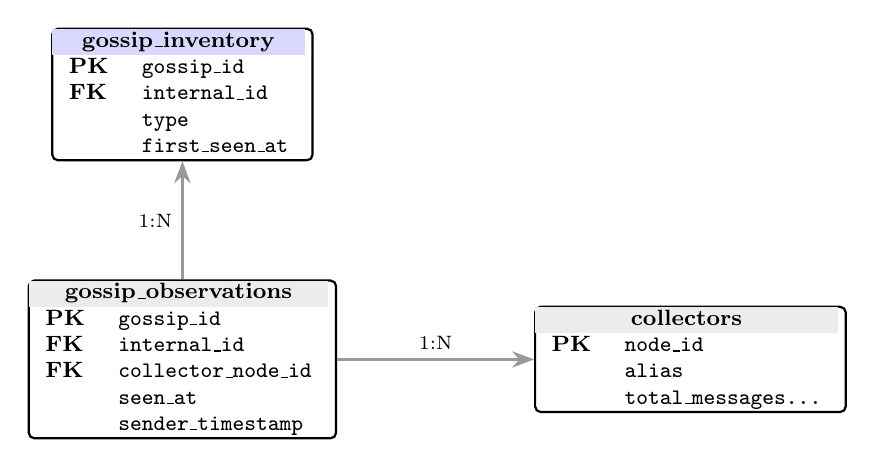
\begin{tikzpicture}[node distance=1.5cm and 2.5cm]

        % 1. Gossip Inventory (The Anchor)
        \node[dbtable] (inventory) {
            \begin{tabular}{l l}
                \rowcolor{blue!15} \multicolumn{2}{c}{\textbf{gossip\_inventory}} \\
                \textbf{PK} & \code{gossip\_id} \\
                \textbf{FK} & \code{internal\_id} \\
                & \code{type} \\
                & \code{first\_seen\_at} \\
            \end{tabular}
        };

        % 2. Gossip Observations
        \node[dbtable, below=of inventory] (observations) {
            \begin{tabular}{l l}
                \rowcolor{gray!15} \multicolumn{2}{c}{\textbf{gossip\_observations}} \\
                \textbf{PK} & \code{gossip\_id} \\
                \textbf{FK} & \code{internal\_id} \\
                \textbf{FK} & \code{collector\_node\_id} \\
                & \code{seen\_at} \\
                & \code{sender\_timestamp} \\
            \end{tabular}
        };

        % 3. Collectors
        \node[dbtable, right=of observations] (collectors) {
            \begin{tabular}{l l}
                \rowcolor{gray!15} \multicolumn{2}{c}{\textbf{collectors}} \\
                \textbf{PK} & \code{node\_id} \\
                & \code{alias} \\
                & \code{total\_messages...} \\
            \end{tabular}
        };

        % Relationships
        \draw[relation] (observations.north) -- (inventory.south) 
            node[midway, left, font=\scriptsize] {1:N};
        \draw[relation] (observations.east) -- (collectors.west)
            node[midway, above, font=\scriptsize] {1:N};

    \end{tikzpicture}
    \caption{
        \textit{Master Registry and Observations}: The \code{gossip\_inventory} 
        acts as the immutable ledger, while \code{gossip\_observations} links 
        messages to the specific \code{collectors} that received them.
    }
    \label{fig:db-master-registry}
\end{figure}
~
The centre of the data model is shown in\autoref{fig:db-master-registry} and begins with 
the \code{gossip\_inventory} table, which functions as an append-only ledger. 
It registers every unique message via its \code{gossip\_id} and assigns a strictly monotonically increasing \code{internal\_id}. 

The \code{gossip\_id} is the \code{SHA256} hash of the raw bytes of the gossip message. 
Due to the nature of this hashing function, a collision is statistically almost impossible to occur,
making this a viable option to uniquely identify and reference a gossip message.

As advocated by \citeauthor{kleppmann_designing_2017}~\cite[Chapter~3]{kleppmann_designing_2017}, 
structuring the core database as an append-only log of immutable events ensures 
robust data integrity and prevents the loss of historical context, 
fulfilling the need for long-term persistence (\ref{req:persistance}).


\subsubsection{Content Tables}
% Content Tables (SCD Type 2)
\begin{figure}[H]
    \centering
    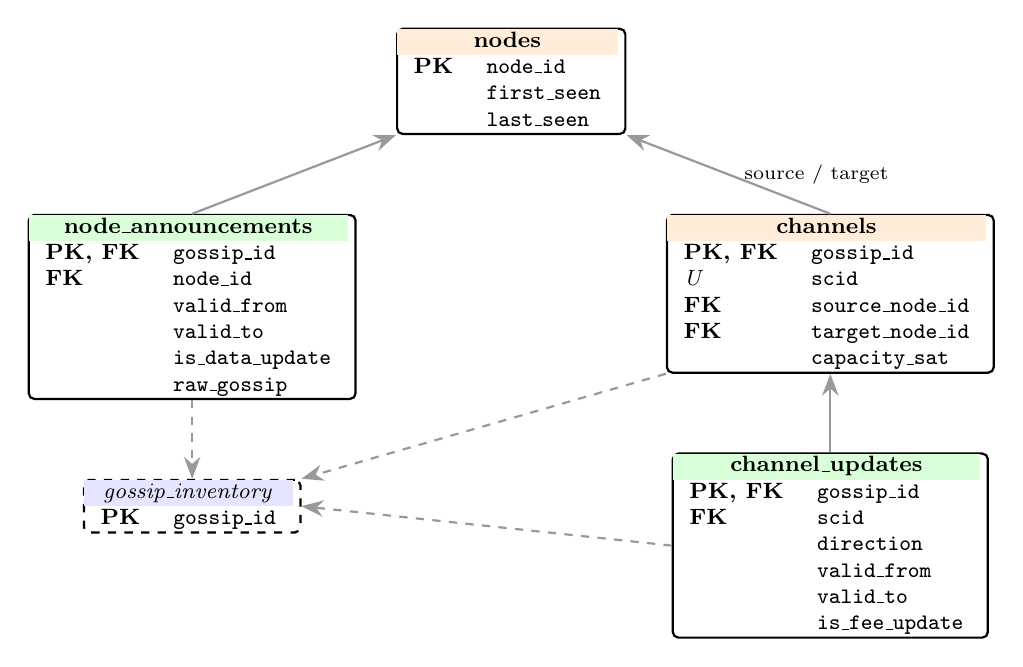
\begin{tikzpicture}[node distance=1.2cm and 0.5cm]

        % 1. Nodes (Top Center)
        \node[dbtable] (nodes) {
            \begin{tabular}{l l}
                \rowcolor{orange!15} \multicolumn{2}{c}{\textbf{nodes}} \\
                \textbf{PK} & \code{node\_id} \\
                & \code{first\_seen} \\
                & \code{last\_seen} \\
            \end{tabular}
        };

        % 2. Node Announcements (Below Left of Nodes)
        \node[dbtable, below left=1cm and 0.5cm of nodes] (nodeann) {
            \begin{tabular}{l l}
                \rowcolor{green!15} \multicolumn{2}{c}{\textbf{node\_announcements}} \\
                \textbf{PK, FK} & \code{gossip\_id} \\
                \textbf{FK} & \code{node\_id} \\
                & \code{valid\_from} \\
                & \code{valid\_to} \\
                & \code{is\_data\_update} \\
                & \code{raw\_gossip} \\
            \end{tabular}
        };

        % 3. Channels (Below Right of Nodes)
        \node[dbtable, below right=1cm and 0.5cm of nodes] (channels) {
            \begin{tabular}{l l}
                \rowcolor{orange!15} \multicolumn{2}{c}{\textbf{channels}} \\
                \textbf{PK, FK} & \code{gossip\_id} \\
                \textit{U} & \code{scid} \\
                \textbf{FK} & \code{source\_node\_id} \\
                \textbf{FK} & \code{target\_node\_id} \\
                & \code{capacity\_sat} \\
            \end{tabular}
        };

        % 4. Gossip Inventory Anchor (Bottom Left, directly below node_announcements)
        \node[dbtable, dashed, below=1cm of nodeann] (inventory2) {
            \begin{tabular}{l l}
                \rowcolor{blue!10} \multicolumn{2}{c}{\textit{gossip\_inventory}} \\
                \textbf{PK} & \code{gossip\_id} \\
            \end{tabular}
        };

        % 5. Channel Updates (Bottom Right, directly below channels)
        \node[dbtable, below=1cm of channels] (chanupd) {
            \begin{tabular}{l l}
                \rowcolor{green!15} \multicolumn{2}{c}{\textbf{channel\_updates}} \\
                \textbf{PK, FK} & \code{gossip\_id} \\
                \textbf{FK} & \code{scid} \\
                & \code{direction} \\
                & \code{valid\_from} \\
                & \code{valid\_to} \\
                & \code{is\_fee\_update} \\
            \end{tabular}
        };

        % Relationships 
        
        % Solid links (Entity relations)
        \draw[relation] (nodeann.north) -- (nodes.south west);
        \draw[relation] (channels.north) -- (nodes.south east) 
            node[midway, right, font=\scriptsize, xshift=2pt] {source / target};
        \draw[relation] (chanupd.north) -- (channels.south);
        
        % Dashed links (Back to Anchor)
        \draw[relation, dashed] (nodeann.south) -- (inventory2.north);
        \draw[relation, dashed] (chanupd.west) -- (inventory2.east);
        \draw[relation, dashed] (channels.south west) -- (inventory2.north east);

    \end{tikzpicture}
    \caption{
        \textit{Content Tables}: This domain implements the \gls{scd} Type 2 architecture. 
        While the temporal boundaries for gossip messages are defined as \code{valid\_from} and \code{valid\_to} 
        in the \code{node\_announcements} and \code{channel\_updates} tables, the \code{channels} table 
        utilizes \code{funding\_timestamp} and \code{closing\_timestamp}.
        All content tables enforce a foreign key relationship back to the \code{gossip\_inventory}.
    }
    \label{fig:db-content-tables}
\end{figure}

The fundamental topological state of the \gls{ln} is preserved within the following tables: 
\code{nodes}, \code{channels}, \code{node\_announcements}, and \code{channel\_updates}
as shown in \autoref{fig:db-content-tables}.

Because the \tech{ln-history} platform is designed to reconstruct historical snapshots,
these tables implement a \gls{scd} Type 2 architecture that allows retaining multiple 
versioned records allows any past state to be accurately derived~\cite[Chapter~11]{kleppmann_designing_2017}. 

Mutable records such as \code{node\_announcements} and \code{channel\_updates} 
are versioned by two boundaries: \code{valid\_from} and \code{valid\_to} 
(\code{channel\_announcements} with \code{funding\_timestamp} and \code{closing\_timestamp}).
These timestamp boundaries ensure that the full topological history is immutably preserved.


\subsubsection{Closure Analysis}
% Closure Analysis
\begin{figure}[H]
    \centering
    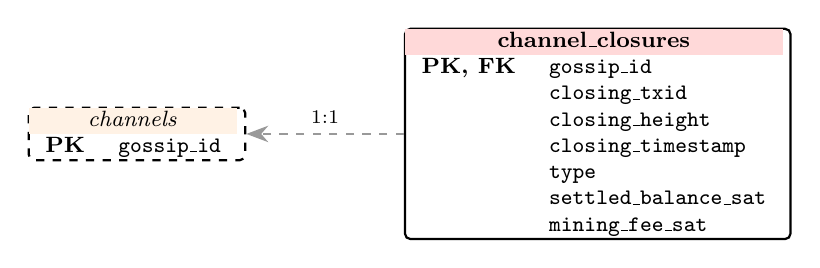
\begin{tikzpicture}[node distance=1.5cm and 2cm]

        % 1. Channel Closures
        \node[dbtable] (closures) {
            \begin{tabular}{l l}
                \rowcolor{red!15} \multicolumn{2}{c}{\textbf{channel\_closures}} \\
                \textbf{PK, FK} & \code{gossip\_id} \\
                & \code{closing\_txid} \\
                & \code{closing\_height} \\
                & \code{closing\_timestamp} \\
                & \code{type} \\
                & \code{settled\_balance\_sat} \\
                & \code{mining\_fee\_sat} \\
            \end{tabular}
        };

        % 2. Channels Anchor (Visual link to Content Tables)
        \node[dbtable, dashed, left=of closures] (channels_anchor) {
            \begin{tabular}{l l}
                \rowcolor{orange!10} \multicolumn{2}{c}{\textit{channels}} \\
                \textbf{PK} & \code{gossip\_id} \\
            \end{tabular}
        };

        % Relationships
        \draw[relation, dashed] (closures.west) -- (channels_anchor.east) 
            node[midway, above, font=\scriptsize] {1:1};

    \end{tikzpicture}
    \caption{
        \textit{Closure Analysis}: The \code{channel\_closures} table stores on-chain settlement data. 
        It is directly linked to the \code{channels} table via the \code{gossip\_id} of the original funding announcement.
    }
    \label{fig:db-closure-analysis}
\end{figure}
The closing transaction reveals information about the channel, that is retrieved
from the Bitcoin blockchain and stored in the \code{channel\_closure} table
which links in a \textit{1:1} relationship to the \code{channels} table
as can be seen in the \autoref{fig:db-closure-analysis}.  


\subsubsection{Peer Operations}
% Peer Operations
\begin{figure}[H]
    \centering
    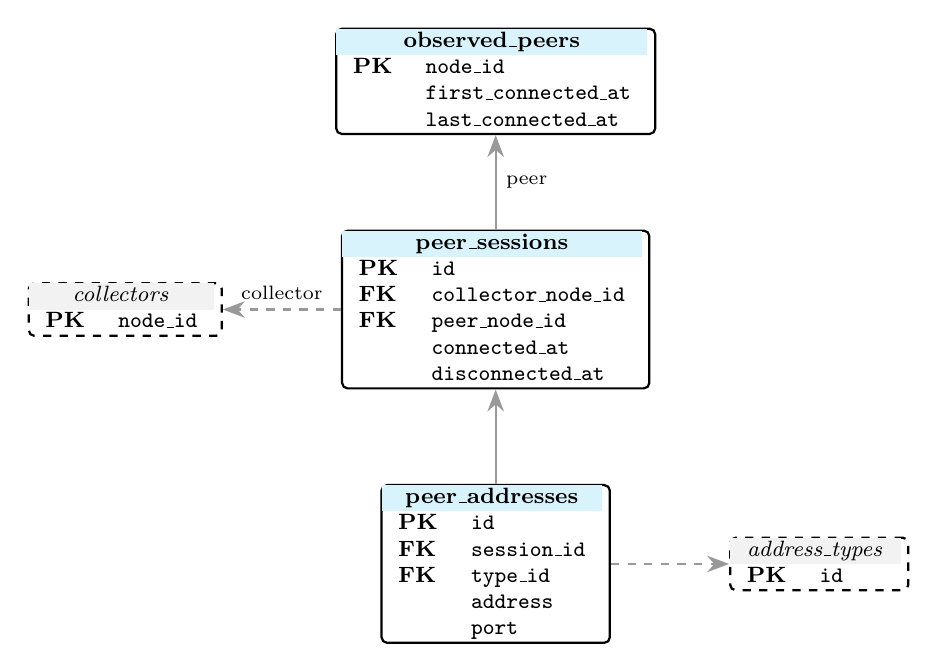
\begin{tikzpicture}[node distance=1.2cm and 1.5cm]

        % 1. Observed Peers (Top)
        \node[dbtable] (observed) {
            \begin{tabular}{l l}
                \rowcolor{cyan!15} \multicolumn{2}{c}{\textbf{observed\_peers}} \\
                \textbf{PK} & \code{node\_id} \\
                & \code{first\_connected\_at} \\
                & \code{last\_connected\_at} \\
            \end{tabular}
        };

        % 2. Peer Sessions (Middle)
        \node[dbtable, below=of observed] (sessions) {
            \begin{tabular}{l l}
                \rowcolor{cyan!15} \multicolumn{2}{c}{\textbf{peer\_sessions}} \\
                \textbf{PK} & \code{id} \\
                \textbf{FK} & \code{collector\_node\_id} \\
                \textbf{FK} & \code{peer\_node\_id} \\
                & \code{connected\_at} \\
                & \code{disconnected\_at} \\
            \end{tabular}
        };

        % 3. Peer Addresses (Bottom)
        \node[dbtable, below=of sessions] (paddresses) {
            \begin{tabular}{l l}
                \rowcolor{cyan!15} \multicolumn{2}{c}{\textbf{peer\_addresses}} \\
                \textbf{PK} & \code{id} \\
                \textbf{FK} & \code{session\_id} \\
                \textbf{FK} & \code{type\_id} \\
                & \code{address} \\
                & \code{port} \\
            \end{tabular}
        };

        % 4. Collectors Anchor (Left of Sessions)
        \node[dbtable, dashed, left=of sessions] (collectors_anchor) {
            \begin{tabular}{l l}
                \rowcolor{gray!10} \multicolumn{2}{c}{\textit{collectors}} \\
                \textbf{PK} & \code{node\_id} \\
            \end{tabular}
        };
        
        % 5. Address Types Anchor (Right of Addresses)
        \node[dbtable, dashed, right=of paddresses] (addrtypes_anchor) {
            \begin{tabular}{l l}
                \rowcolor{gray!10} \multicolumn{2}{c}{\textit{address\_types}} \\
                \textbf{PK} & \code{id} \\
            \end{tabular}
        };

        % Relationships 
        
        % Solid links (Entity relations)
        \draw[relation] (sessions.north) -- (observed.south) 
            node[midway, right, font=\scriptsize] {peer};
        \draw[relation] (paddresses.north) -- (sessions.south);
        
        % Dashed links (Back to Anchors)
        \draw[relation, dashed] (sessions.west) -- (collectors_anchor.east) 
            node[midway, above, font=\scriptsize] {collector};
        \draw[relation, dashed] (paddresses.east) -- (addrtypes_anchor.west);

    \end{tikzpicture}
    \caption{
        \textit{Peer Operations}: This domain tracks real-time connectivity. 
        A \code{peer\_session} records the exact timeframe a connection was 
        active between an \code{observed\_peer} and an internal \code{collector}.
    }
    \label{fig:db-peer-ops}
\end{figure}

The \gls{cln} nodes regularly switch between peers to receive gossip messages.
To persist this information, specifically the session data, the data model shown in
\autoref{fig:db-peer-ops} is deployed in the \service{ln-history-database}.



\subsection{Indexing}
To satisfy the dual requirements of high-throughput real-time ingestion (\gls{oltp}) 
and complex historical analysis (\gls{olap}) without blocking each other (\ref{req:concurrency}), 
the schema employs custom B-Tree indexes.

B-Trees are the industry standard for database indexing, providing logarithmic time complexity 
for both exact matches and range queries~\cite[Chapter~14]{garcia-molina_database_2009}.
Primary keys enforce referential integrity across the database, ensuring that duplicate \code{gossip\_id}s are always rejected.

Beyond structural constraints, composite indexes are heavily utilized to accelerate snapshot queries. 
For example, the \code{channel\_updates} table owns the \code{idx\_chan\_upd\_lookup} index on the column triple \code{(scid, direction, valid\_to)}, 
as well as the \code{idx\_chan\_upd\_validity} index combining \code{(valid\_from, valid\_to)}. 
Likewise, the \code{node\_announcements} table utilizes the \code{idx\_node\_ann\_validity} index on \code{(valid\_from, valid\_to)}
and the \code{channel\_announcements} table \code{idx\_chan\_val\-id\-ity} on \code{(funding\_timestamp, closing\_timestamp)}.

Joining tables is a necessary operation for in-depth analytical queries 
but can rapidly become a performance bottleneck if executed on suboptimal data types~\cite[Chapter~15]{garcia-molina_database_2009}.
Using the \code{gossip\_id}, which is a \code{SHA256} hash, is of datatype \code{varchar(64)}, 
as a joining column is significantly more expensive than joining on a \code{bigint} column. 
The reason for this is, that string comparisons require sequential byte-by-byte evaluation. 
Therefore, an \code{internal\_id} of type \code{bigint} (\tech{PostgreSQL}'s native 8-byte integer) 
was introduced as the primary joining key. 
Integer comparisons are executed natively at the CPU register level, 
yielding orders of magnitude faster join operations~\cite[Chapter~15]{garcia-molina_database_2009}.


\subsection{Clustering}
The data retrieval for historical snapshots is exceptionally fast due to the utilization 
of the \tech{PostgreSQL} \code{CLUSTER} command~\cite{cluster_postgresql_2026}.
While standard B-Tree indexes optimize the logical search path, they do not dictate the physical storage layout on the hard drive. 
Over time, as out-of-order gossip messages are ingested and historical gaps are filled, the tables naturally suffer from physical fragmentation.

By executing the \code{CLUSTER} command against the temporal validity indexes (such as \code{idx\_chan\_upd\_validity}), 
the database physically reorders the table rows on disk to perfectly mirror the logical index sequence. 
As detailed by Garcia-Molina et al.~\cite[Chapter~13]{garcia-molina_database_2009}, 
this physical clustering ensures that the physical location of a row correlates with the logical value of the \code{valid\_from} column.
The correlation is a value in the interval $[-1,1]$. 
As long as it is close to $-1$ or $1$ the physical value is close to 
Consequently, when analytical queries request vast time-windows of the network's history, 
the database can fetch the requested data utilizing highly efficient, sequential disk I/O reads, 
skipping random disk seeks.



\section{Data Enrichment}

\subsection{Data Enrichment from the Blockchain \service{chain-enricher}}
\label{sec:chain-enricher}

The operational footprint of the \gls{ln} on the Bitcoin blockchain is limited to two events: 
the \textit{funding} and the \textit{closing} of a channel. 

Because Lightning nodes rely on their underlying Bitcoin nodes to observe these events, 
specific on-chain metrics such as channel capacity or closure details
are omitted from the gossip protocol to reduce network bandwidth~\cite{antonopoulos_mastering_2021}.

The motivation for the \service{chain-enricher} is to seperate the gathering of on-chain information from the \service{gossip-processor}. 
The \service{chain-enricher} is written in python and its source code can be found here~\cite{kraus_chainenricher_2026}. 
It operates via concurrent worker threads that asynchronously query indexed blockchain data, 
enriching the \service{ln-history-database} with metadata without disturbing the real-time gossip ingestion.

\subsubsection{Funding Transaction Resolution}
To retrieve missing funding data, the \service{chain-enricher} continuously polls 
the database for channels lacking capacity or funding timestamp information. 
To optimize retrieval latency, the enrichment process is divided into a high-performance primary workflow (\term{fast path}) 
and a secondary fallback mechanism (\term{slow path}), 
determined by the availability of the participating nodes' on-chain public keys.

\paragraph{Primary Retrieval (Fulcrum Indexer)}
If both \code{bitcoin\_key\_1} and \code{bitcoin\_key\_2} are present in the channel's gossip data, 
the funding worker utilizes the fast path. 
It reconstructs the channel's 2-of-2 multisignature \gls{p2wsh} address by sorting the raw keys lexicographically 
in accordance with BIP67 rules~\cite{kerin_bip_2015}, and hashing the resulting witness script. 
Using this derived script hash, the enricher queries \tech{Fulcrum}~\cite{culianu_cculianu_2026}, 
a high-speed Electrum server implementation that maintains a fast, queryable index of the entire Bitcoin blockchain. 
By evaluating the transaction history of this script hash, the earliest confirmed entry is identified as the funding transaction. 
To maximize throughput, these queries are executed concurrently across multiple threads.

\paragraph{Fallback Retrieval (Bitcoin Core RPC)}
If the primary retrieval fails, the service falls back to a secondary method that leverages the structural properties of the \gls{scid}. 
As elaborated in \autoref{sec:gossip-messages}, the $64$-bit \gls{scid} deterministically encodes the block height, transaction index, and output index. 
The worker decodes this identifier and issues a sequence of batched JSON-RPC queries (\code{getblockhash}, \code{getblock}, and \code{getrawtransaction}) 
directly to a local Bitcoin Core node to locate the exact funding output.

Independently of the retrieval path utilized, the raw transaction is parsed to extract the value of the 
specific output (\code{capacity\_sat}) and the block confirmation time (\code{funding\_timestamp}). 
These metrics are then persisted into the \code{channels} table.

\subsubsection{Closure Detection and Classification}
Detecting when and how a channel is closed via raw blockchain data is highly resource-intensive, 
as it would natively require exhaustive \gls{utxo} set lookups. 
A more scalable closure detection is utilized by the \service{chain-enricher} by again using the \tech{Fulcrum} index.

For every active channel in the database with known Bitcoin keys, the closure worker utilizes the previously discussed \gls{p2wsh} script hash derivation. 
By querying \tech{Fulcrum} for the transaction history of this specific script hash, 
the service can instantly find out if the funding output has been spent. 
If a spending transaction is detected, the channel is marked as closed.

Furthermore, the service classifies the type of closure (e.g., bilateral/mutual or unilateral/force close) 
by analysing the \code{nSequence} field of the spending input. 
As mandated by the BOLT\#3 specification~\cite{lightningdevelopers_bolt-3_2026}, 
mutual closures utilize an \code{nSequence} value of \code{0xFFFFFFFF} or \code{0xFFFFFFFE}, 
whereas unilateral closures encode the commitment number, resulting in strictly lower sequence values. 
Additionally, the on-chain mining fee is derived by subtracting the settled output values from the initial channel capacity.

\subsubsection{Discussing Performance Considerations}
Empirically, this indexed approach has reduced I/O latency. 
While the \tech{Fulcrum} index approximately \qty{100}{\giga\byte} of extra storage (Bitcoin blockchain takes around \qty{600}{\giga\byte} as of writing),
the retrieval optimizations allow the \service{chain-enricher} to process historical data rapidly. 
In production benchmarking, the service successfully derived and enriched over $200000$ channel fundings and closings states in just a few hours.



\subsection{Peer Session Enrichment: \service{peer-manager}}
\label{sec:peer-manager}

The \service{peer-manager} service is implemented in \tech{Python} and the source code can be found at~\cite{kraus_peermanager_2026}. 
Its responsibility is to monitor and record the \gls{p2p} connections done by the underlying \gls{cln} collector nodes.

In the \gls{ln}, nodes are not strictly obligated to forward gossip messages, and \gls{p2p} connections are often ephemeral. 
Different client implementations utilize varying algorithms for peer rotation, 
meaning the network topology observed by a single node is heavily dependent on its active connections. 
As demonstrated later in \autoref{ch:empirical-data-analysis}, 
the specific peers a node is connected to directly influence the volume and latency of the gossip it receives. 
To analyse this empirical data, the \service{peer-manager} persists session metadata 
including peer identifiers, connection durations, and network address types into the \service{ln-history-database}.
Details about the data model can be found in \autoref{fig:db-peer-ops}.

\paragraph{Polling and Session Management}
The service communicates directly with the \gls{cln} nodes via the native \tech{JSON-RPC} interface using the \tech{pyln-client} library. 
It executes a polling loop at a fixed interval, repeatedly requesting the \code{listpeers} RPC method. 
By comparing the array of currently connected peers against the open sessions in the database, the service detects changes. 

When a new connection is identified, the service parses the raw network address strings and determines the routing protocol. 
When a peer disappears from the active list, the corresponding database session is gracefully closed by appending a \code{disconnected\_at} timestamp.

\paragraph{Targeted Reconnection and Observability}
Beyond passive monitoring, the service provides an active auto-reconnection feature. 
By configuring a local target list (\file{target\_peers.json}), 
researchers can define specific nodes the collector should try to connect to. 
During each polling cycle, the \service{peer-manager} verifies connectivity to these targets 
and automatically issues \code{connect} RPC commands if a session has dropped. 

 

\section{Serving \& Using the Platform}

After the gossip data has been successfully ingested and enriched within the database, the focus shifts to data accessibility. 
First, \autoref{sec:ln-history-api} details the \service{ln-history-api}, which interfaces with the database to provide a high-performance \textit{RESTful} API. 
Subsequently, \autoref{sec:ln-history-python-client} introduces a custom \tech{Python} library designed to easily parse and analyse the binary results returned by the API.

\subsection{Serving analytical results: \service{ln-history-api}}
\label{sec:ln-history-api}

The \service{ln-history-api} serves as the primary backend interface for external clients. 
It is implemented in \tech{C\#} using the \tech{.NET} framework~\cite{microsoftcorporation_net_2026}, 
with the open-source code available at~\cite{kraus_lnhistoryapi_2026}. 
The service adheres to the standard \gls{mvc} architectural pattern.

\paragraph{Data Access and Performance Optimization}
Given the sheer volume of historical gossip data, traditional \gls{orm} 
like the \tech{Entity Framework} introduce prohibitive memory and processing overheads. 
Therefore, the API bypasses heavy \glspl{orm}, opting instead for a combination of 
\tech{Dapper} (a lightweight micro-ORM) and the native \tech{Npgsql} driver. 
This architecture allows the controllers to execute highly optimized SQL queries and 
map results directly to lightweight \gls{dto}. 

Furthermore, all endpoints are strictly instrumented using custom \code{AppMetrics}. 
The API actively monitors and logs the duration of database query planning versus actual data streaming,
exposing this telemetry to the system's observability stack which gets explained later in \autoref{sec:observability}.

\paragraph{Historic Timestamp Queries}
A core feature of the API is its ability to reconstruct the exact state of network at any specific historical timestamp, 
satisfying the snapshot retrieval requirement (\ref{req:snapshot}).

The \code{NodeController} and \code{ChannelController} expose endpoints that query the \gls{scd} Type 2 database schema. 
This allows clients to efficiently filter by specific identifiers (\ref{req:entity-filtering}) and 
retrieve overlapping time-windows of gossip data (\ref{req:snapshot-diff}).

\paragraph{Snapshot Streaming}
The most resource-intensive operation is the generation of full network snapshots, managed by the \code{LightningNetworkController}. 
To prevent memory exhaustion (\gls{oom} crashes) when retrieving megabytes of binary \code{raw\_gossip} data, the API utilizes a direct streaming architecture.
This ensures the platform remains resource-efficient and capable of running on consumer-grade hardware (\ref{req:self-host}).

Rather than materializing huge \code{UNION} datasets into the server's RAM, 
the API leverages the native PostgreSQL \code{COPY} protocol (\code{BeginRawBinaryCopyAsync}) 
to stream data byte-by-byte directly to the client's HTTP response stream as an \code{application/octet-stream}. 


\subsection{Using the results: \service{ln-history-python-client}}
\label{sec:ln-history-python-client}

The \service{ln-history-python-client} library~\cite{kraus_lnhistorypythonclient_2026} 
main objective is to be the interface for parsing raw binary gossip data and interacting with the \service{ln-history-api}.
While the current reference implementation is written in \tech{Python}, the architectural patterns are strictly typed and designed to be portable
 to other strongly-typed languages such as \tech{TypeScript} or \tech{C\#}.

\subsubsection{Data Models and Interfaces}
The \code{./model} module defines the data structures representing the Lightning network protocol. 
It utilizes Python \term{dataclasses} to strictly type the deserialized binary fields of
messages such as \code{ChannelAnnouncement}, \code{NodeAnnouncement}, and \code{ChannelUpdate}. 

To support the specific architecture of this thesis, the module includes a specialized \code{core\_lightning\_internal} submodule, 
which handles the non-standard, internal message formats used exclusively by \gls{cln} nodes (e.g., \code{channel\_amount} or \code{channel\_dying}).
Furthermore, the models implement \code{@property} decorators that abstract complex bitwise operations for the end-user. 
For example, the \code{ChannelUpdate} model automatically extracts the directional routing bit from the raw \code{channel\_flags} byte, 
and the \code{ChannelAnnouncement} model translates the 64-bit integer \gls{scid} into a human-readable block height format. 

Lastly, each model implements serialization methods (\code{to\_dict}) to help debugging and database insertion.

\subsubsection{Parsing Strategy}
Deserializing raw byte streams into structured objects is heavily optimized within the \code{parser} directory. 
Instead of relying on monolithic evaluation blocks, the library implements an extensible \textit{Factory Pattern} (\file{parser\_factory.py}). 

By inspecting the first two bytes of a raw message, the factory determines the message type and 
dynamically routes the byte stream (\code{io.BytesIO}) to the corresponding parser defined in \file{parser\_map.py}. 
The individual parsers then utilize Python's \code{struct.unpack} library to safely extract \gls{be} integers and cryptographic signatures.

Additionally, to handle massive historical datasets, the \code{read\_gossip\_file} function provides 
an interface for iterating over various storage formats:
\begin{enumerate}
    \item The \gls{cln} \file{gossip\_store} binary format.
    \item The \term{GSP-format} proposed by \citeauthor{decker_lnresearch_2020}.
    \item Standard varint-delimited messages.
\end{enumerate}
This iterator implementation is optimized for memory efficiency by utilizing the \code{yield} statement. 
Inspired by the \term{time-machine} tool~\cite{decker_lnresearch_2020}, 
it allows the sequential processing of multi-gigabyte files without loading the entire dataset into \gls{ram}.

\subsubsection{API Interaction}
To abstract the complexity of HTTP communication and binary deserialization, 
the client provides the \code{LnHistoryRequester} class.

\begin{listing}[htbp]
    \begin{minted}[frame=lines, fontsize=\footnotesize]{python}
        def get_snapshot_at_timestamp(
                self,
                timestamp: datetime,
                return_graph: bool = True,
                save_to_file: Optional[str] = None,
                format: Optional[str] = None,
                stopwatch: Optional[bool] = False,
            ) -> Union[nx.DiGraph, str]:
    \end{minted}
    \caption{
        Method definition for retrieving historic network snapshots. 
        The method supports direct deserialization into graph structures for immediate topological analysis~\cite[./LnHistoryRequester.py]{kraus_lnhistorypythonclient_2026}.
    }
    \label{lst:get_snapshot_at_timestamp_header}
\end{listing}

As shown in \autoref{lst:get_snapshot_at_timestamp_header}, the \code{get\_snapshot\_at\_timestamp} method 
allows researchers to retrieve a full network snapshot from the \service{ln-history-api}.
This method natively parses the incoming binary stream and directly deserializes it into a 
\tech{NetworkX}~\cite{hagberg_exploring_2008} directed graph (\code{nx.DiGraph}), 
allowing researchers to immediately begin topological analysis without writing boilerplate parsing code.

\subsubsection{Distribution}
The library is packaged and distributed via the Python Package Index (\gls{pypi})~\cite{pythonpackagingauthority_pip_2024}, 
allowing for modular installation in other components of the system via \code{pip install lnhistoryclient}.


\section{Observability: Monitoring, Logging, Tracing}
\label{sec:observability}

The \tech{ln-history} platform is designed to constantly process high volumes of network data. 
Monitoring that all components work properly is crucial to ensure a smooth and uninterrupted service. 
To achieve this, the architecture implements tools for \textit{Metrics}, \textit{Logs}, and \textit{Traces} alongside a centralized visualization layer.

\begin{enumerate}
    \item \textbf{Metrics (\tech{Prometheus}):} 
        Metrics provide quantitative data about the system's performance over time (e.g., CPU usage, active connections, messages processed per second). 
        The platform utilizes \tech{Prometheus}, an industry-standard time-series database, to scrape and centrally store these metrics from all running services.

    \item \textbf{Logs (\tech{Loki} \& \tech{Promtail}):} 
        Logs provide immutable, timestamped records of discrete events. 
        To prevent logs from being isolated inside individual Docker containers, 
        \tech{Promtail} is used as an agent to gather log streams and forward them to \tech{Loki}, 
        a highly efficient log aggregation system designed to integrate seamlessly with \tech{Prometheus}.

    \item \textbf{Traces (\tech{OpenTelemetry}):} 
        Traces track the progression of a single request across multiple distributed services. 
        This is particularly useful for analysing which API endpoints are accessed at what frequency, 
        and for identifying exact latency bottlenecks within the \service{ln-history-api} service.

    \item \textbf{Dashboards (\tech{Grafana}):} 
        \tech{Grafana} acts as the unified presentation layer, offering many visualization styles
         to query and display the data collected by the aforementioned systems.
\end{enumerate}

\paragraph{Motivation and Implementation in the Architecture}
These observability tools have been integrated into the following components: 
\service{peer-manager}, \service{chain-enricher}, and \service{gossip-processor}. 

A naive approach to monitor the system would be to execute repetitive queries 
(e.g., \code{COUNT(*)}) directly against the \service{ln-history-database} 
to make sure the system is still running. 
However, this is considered an architectural anti-pattern for data-intensive applications~\cite[Chapter~3]{kleppmann_designing_2017}. 
Executing frequent analytical queries on an active operational database severely exhausts its resources 
and directly degrades the throughput of the real-time ingestion pipelines. 
Instead, we let the \tech{Python} and \tech{.NET} services expose metrics natively to \tech{Prometheus}. 
This separation of concerns ensures that the platform remains performant 
while simultaneously enableing an administrator to monitor the live status via a public dashboard\footnote{\url{https://app.ln-history.info}}.



\section{Deployment}
\label{sec:deployment}

To fulfil the non-functional requirement of environment-agnostic deployability (\ref{req:docker}), 
the entire \tech{ln-history} infrastructure is defined declaratively using a single 
\file{docker-compose.yaml} file\footnote{The complete compose file is available at \url{https://ln-history.info/docker-compose.yaml}}.

\paragraph{Orchestration and Versioning}
All custom components developed for this thesis are containerized as individual \tech{Docker} images 
and strictly versioned to guarantee reproducible deployments and long-term maintainability (\ref{req:maintainability}).
The entire stack can be initialized with a standard \code{docker compose up -d} command. 
To prevent race conditions during startup, the orchestration leverages the \code{depends\_on} attribute, 
ensuring that services boot sequentially and only after their respective dependencies are fully working. 
Furthermore, sensitive configuration data, such as database credentials and RPC passwords, 
are securely managed and injected at runtime via a local \file{.env} file.

\paragraph{External Prerequisites}
While the \tech{ln-history} platform is almost self-contained, 
it inherently relies on the Bitcoin base layer to function. 
A mandatory prerequisite for deployment is an accessible Bitcoin Core node with configured RPC authentication,
coupled with a fully synced, Electrum-compatible blockchain indexer (specifically \tech{Fulcrum}). 
As detailed in \autoref{sec:chain-enricher}, these external services provide the on-chain data necessary for resolving channel capacities and closures.

\paragraph{Network Isolation and Static IP Routing}
A unique architectural challenge when running multiple \gls{cln} collector nodes on a single physical server 
is managing their public network presence.
For the \gls{ln} gossip protocol to function without errors, nodes must have distinct, static public IP addresses. 
To achieve this and maintain scalability, the deployment architecture utilizes a sidecar proxy network pattern. 
Instead of exposing the local server to the internet, each \gls{cln} container is isolated 
from the host network and bound to a dedicated \tech{WireGuard} \gls{vpn} container. 
These \gls{vpn} gateways route the Lightning node traffic exclusively through small, remotely rented \gls{vps} instances. 
This approach efficiently provisions each local collector node with its own static IPv4 address, allowing the platform
to scale horizontally on a single machine while appearing as topologically distinct routing nodes to the public \gls{ln}.
	\chapter{Empirical Data Analysis}
\label{ch:empirical-data-analysis}

This chapter showcases the analytical possibilities of the \tech{ln-history} platform. 
By using the \service{ln-history-database} and \service{ln-history-api}, 
we conduct novel analyses of the \gls{ln} and update existing findings from previous literature. 
All analytical scripts and raw data underlying this chapter are available as open-source code\footnote{\url{https://ln-history.info/analysis}}.
The analysis is divided into two scopes:

\begin{itemize}
    \item \textbf{Short-Term Metadata (\autoref{sec:metadata-analysis}):} 
        Focuses on the real-time operational behaviour of the network and the performance of the gossip protocol over a constrained collection window.

    \item \textbf{Long-Term Topology (\autoref{sec:historic-gossip-analysis}):} 
        Examines the macroscopic evolution of the network graph from its inception to the present day.
\end{itemize}

\subsection*{Scope and Methodology}

The first section (\autoref{sec:metadata-analysis}) is limited to the continuous collection window 
maintained by the two \tech{ln-history} collector nodes. 
This window starts on January 14, 2026, to March 3, 2026, during which the platform operated without major outages. 
Both nodes were deployed using the default \gls{cln} (\code{v25.09}) configuration, 
meaning they actively maintained connections to ten peers to receive gossip messages. 

By utilizing the metadata enriched during this period, we examine the total volume of messages 
and the degree of data overlap between the two distinct points in the topology (\autoref{fig:network-gossip-volume-and-overlap}). 
After that, we calculate the absolute propagation lag of the \gls{ln} (\autoref{fig:propagation-lag}) 
and the inter-collection lag between our two collector nodes (\autoref{fig:inter-collection-lag}). 
Finally, we analyse node connectivity behaviour by showing the distribution of peer session lengths (\autoref{fig:peer-session-distribution}) 
and testing for correlations between session duration and overall node capacity (\autoref{fig:peer-session-correlation}).


The second section (\autoref{sec:historic-gossip-analysis}) utilizes the batch-import 
capabilities of the platform to dive into the historical evolution of the \gls{ln} topology. 
We establish a baseline by showing the overall volume and distribution of historic gossip messages (\autoref{fig:gossip-messages-distribution}). 
Using the platform's snapshot functionality, we focus on payment channels, 
which build the routing backbone of the \gls{ln}. 
By examining the channel lifetime distribution (\autoref{fig:channel-lifetime-distribution}), 
we gain insights into the capital efficiency of the network. 
We also investigate whether the capacity of a channel influences correlates 
with the lifetime of a channel lifetime (\autoref{fig:channel-lifetime-correlation}). 
We finish off by acknowledging that the \gls{ln} is a distributed and not strictly decentralized network, 
we analyse its structural centralization over time. 
Building upon the methodology introduced by \citeauthor{zabka_short_2022}~\cite{zabka_short_2022}, 
we calculate the Gini coefficient based on the \gls{bc} for each historical snapshot (\autoref{fig:betweenness-centrality-gini}) 
and track the share of total \gls{bc} commanded by the top percentiles of routing nodes (\autoref{fig:betweenness-centrality-top-percentiles}).
We see that only a handful of nodes are very central in the \gls{ln} and visualize their
dominance over time in a heatmap, see \autoref{fig:top-nodes-heatmap}.


\section{Gossip Metadata Analysis}
\label{sec:metadata-analysis}

We introduced the gossip protocol in \autoref{sec:ln-gossip-protocol}, showing 
how storage efficient the topology information is. 
%AVG length of the raw_bytes column * number of messages in time frame * 0.8
We begin by exploring the collected gossip messages, shedding light into the volume
as well as completeness.
First we quantify the daily message volume and empirically measure the message propagation across the network. 
Theoretically, the \gls{ln} gossip protocol aims for global \textit{consensus}, 
meaning every node should eventually receive every broadcasted message.


\subsection{Network Gossip Volume and Lag}

We start by showing the number of gossip messages in the time frame to estimate the baseline network volume. 
To assess propagation consistency, we evaluate the intersection of messages received 
by our two independent collector nodes (referred to as \textit{Alice} and \textit{Bob}).

\subsubsection{Network Gossip Volume and Overlap}

Both collector nodes operate independently and 
append a local \code{seen\_at} timestamp as soon as they receive a gossip message. 
This gives three scenarios: 
A gossip message may be observed exclusively by Alice, exclusively by Bob, or (successfully) by both nodes.

\begin{figure}[htbp]
    \centering
    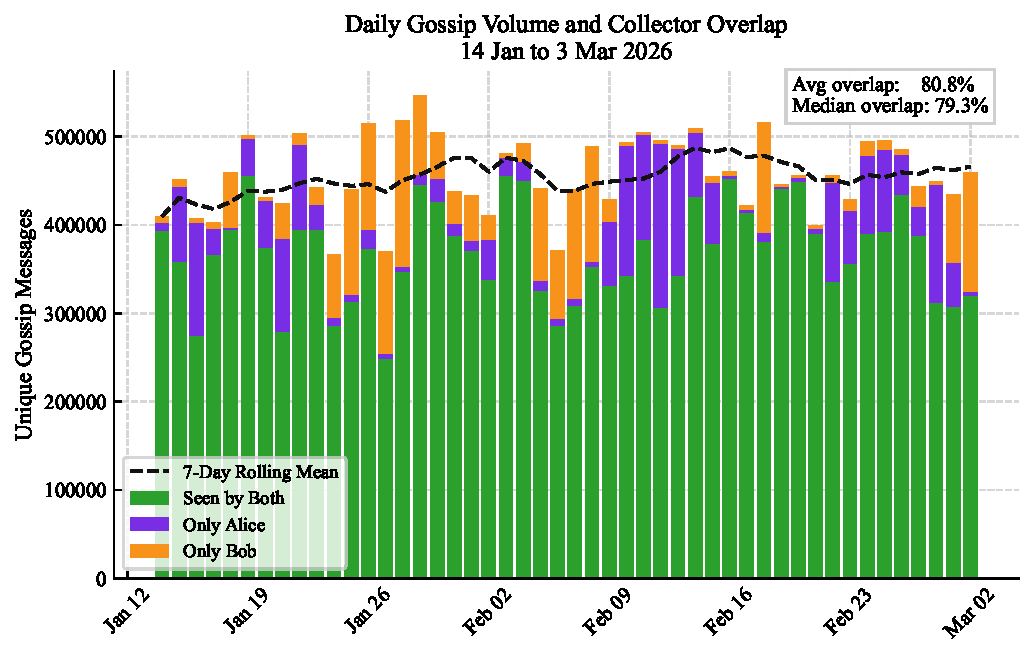
\includegraphics[width=0.7\linewidth]{resources/results-final/network-gossip-volume-and-overlap.pdf}
    \caption {
        In the measured time window around $400000$ unique messages have been seen by both nodes.
        The overall share of messages that have been received by both nodes is around $80\%$.
        Neither collector node has had an advantage sometimes Alice saw more, sometimes Bob. 
    }
    \label{fig:network-gossip-volume-and-overlap}
\end{figure}

The \autoref{fig:network-gossip-volume-and-overlap} shows that the rate of messages per day is rather constant
with a 7-day rolling average fluctuating between $400000$ and $500000$ unique messages.
The average overlap of $80.8 \%$ (median $79.3 \%$) shows that there are significant gaps in the gossip propagation.

We can also utilize the dataset to estimate the bandwidth requirements for operating a \gls{ln} node. 
\autoref{tab:message-footprint} presents the storage and message distribution grouped by type.

\begin{table}[htbp]
    \centering
    \caption{Storage footprint and message volume by gossip message type over the 48-day measurement window.}
    \begin{tabular}{@{} l r r r @{}}
        \toprule
        \textbf{Name} & \textbf{Avg Size (B)} & \textbf{Unique Msgs.} & \textbf{Total (MB)} \\
        \midrule
        Channel Announcement & 435.0 & \num{13045}     & 5.67    \\
        Node Announcement    & 502.3 & \num{6575334}  & 3302.95  \\
        Channel Update       & 143.0 & \num{14493905} & 2073.23  \\
        \bottomrule
    \end{tabular}
    \label{tab:message-footprint}
\end{table}

As \autoref{tab:message-footprint} shows, the total downloaded payload is \qty{4863}{\mega\byte} for Alice 
and \qty{4749}{\mega\byte} for Bob over the \num{48} consecutive days of measurement. 
This translates to a daily bandwidth requirement of roughly \qty{101.3}{\mega\byte} (\qty{98.9}{\mega\byte} respectively).
At the protocol level, this requires the node to process an average of \qty{4.6}{\text{messages}\per\second}. 
This demonstrates that the necessary bandwidth to run a \gls{ln} node, remains 
well within the constraints of standard consumer-grade internet connection.


\subsubsection{Propagation Lag}

When discussing protocol improvements it is useful to look at empirical measurements.
The propagation lag is calculated as the difference between the timestamp of the sender node $t_{sender}$
and the timestamp when a collector node has seen it $t_{seen}$: $|t_{seen} - t_{sender}|$.

In case both collector nodes have seen it at timestamp $t_{Alice}$ and $t_{Bob}$,
the first timestamp is chosen $t_{seen} = \min(t_{Alice}, t_{Bob})$. 

We group these measurements by message type, 
as each type serves a fundamentally different operational role within the network.

\begin{figure}[htbp]
    \centering
    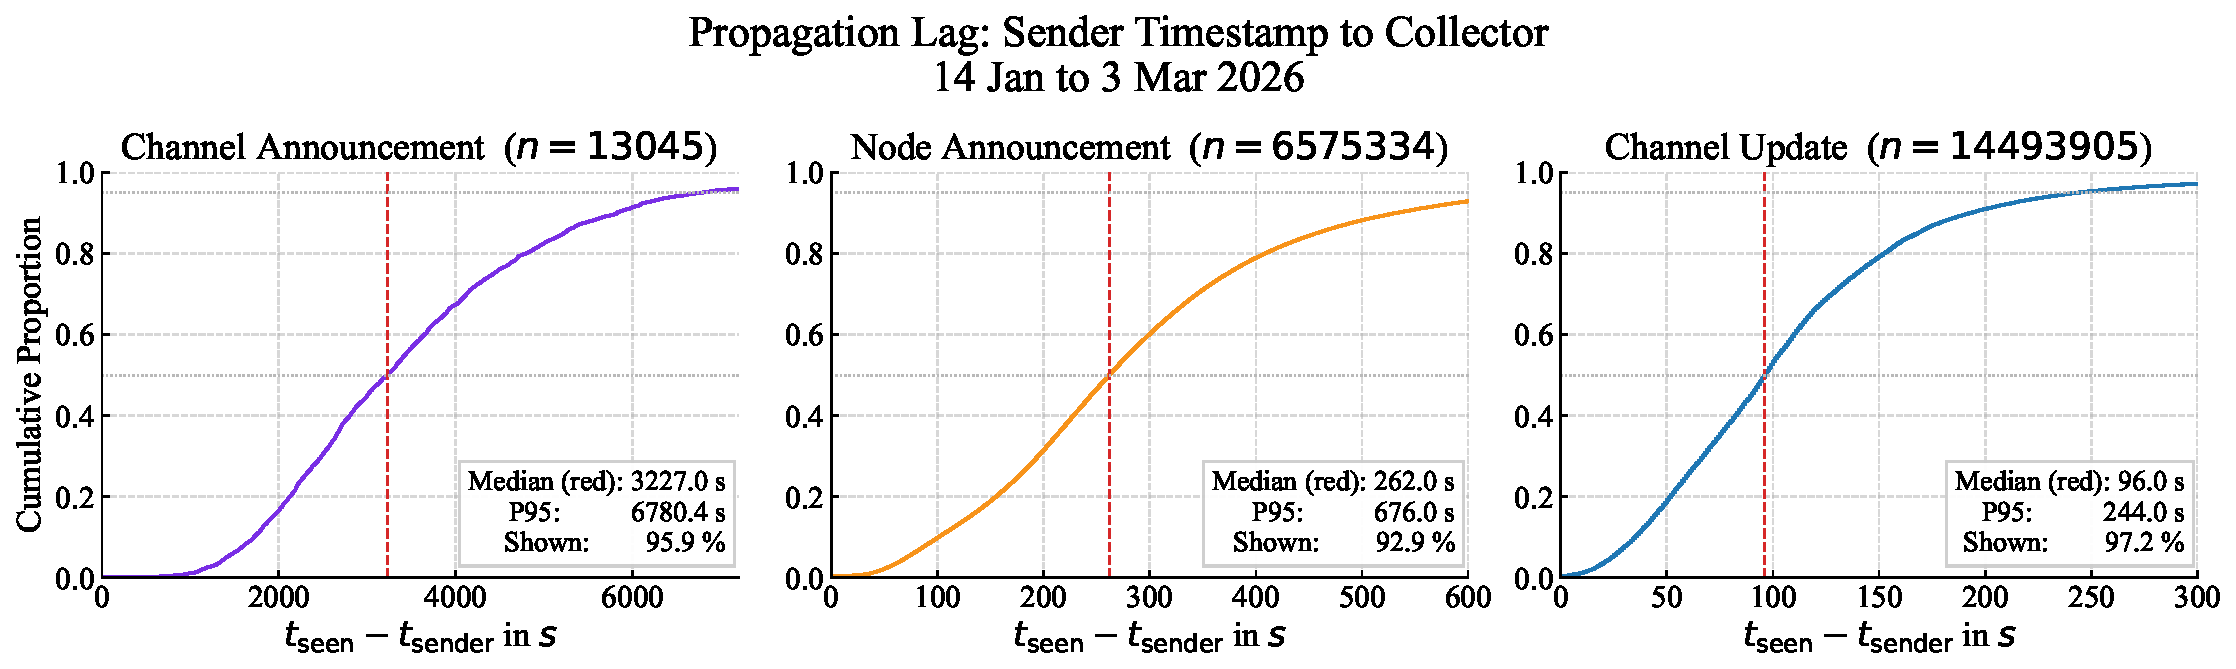
\includegraphics[width=\textwidth]{resources/results-final/propagation-lag-large.pdf}
    \caption{
        The Lag between the message type differs enormously depending on the message type.
        \code{Channel\_announcements} take on median around \qty{3227}{\second} and are an order of magnitude 
        slower than \code{node\_annoncements} and \code{channel\_updates} which respectively 
        only have (on median) \qty{262}{\second} and \qty{96}{\second}.
    }
    \label{fig:propagation-lag}
\end{figure}

\autoref{fig:propagation-lag} illustrates the propagation lag in a \gls{cdf} chart grouped my messages type.
\code{Channel\_announcement} propagation is much slower with \qty{3227}{\second} 
(approximately \num{54} minutes) due to the on-chain footprint.
As mandated by the BOLT specification, nodes must wait for six block confirmations
before broadcasting the announcement to the public network~\cite{lightningdevelopers_bolts_2018}. 
This mandatory waiting period artificially inflates the measured propagation lag.

It is also notably to see how steep the curves grow.
As \code{node\_announcements} are in most cases heartbeats with redundant information 
it is less urgent for them to spread quickly resulting in a lag of \qty{262}{\second} (more than \num{4} minutes).
But as \code{channel\_updates} play an important role in routing payments, their information spreading is urgent
achieving a median lag of only \qty{96}{\second}.


\subsubsection{Inter Collection Lag Distribution}
While absolute propagation lag measures the delay from the origin, 
the \term{inter-collection lag} evaluates the synchronization between the two independent
positions of \textit{Alice} and \textit{Bob} in the \gls{ln}. 

It is defined as the absolute difference between the collection timestamps of Alice and Bob
for a given unique message: $|t_{Bob} - t_{Alice}|$. 

This metric could answer whether two distinct, standardly configured \gls{cln} nodes receive 
the same network updates concurrently or if there is a significant synchronization delay between different network clusters.

\begin{figure}[htbp]
    \centering
    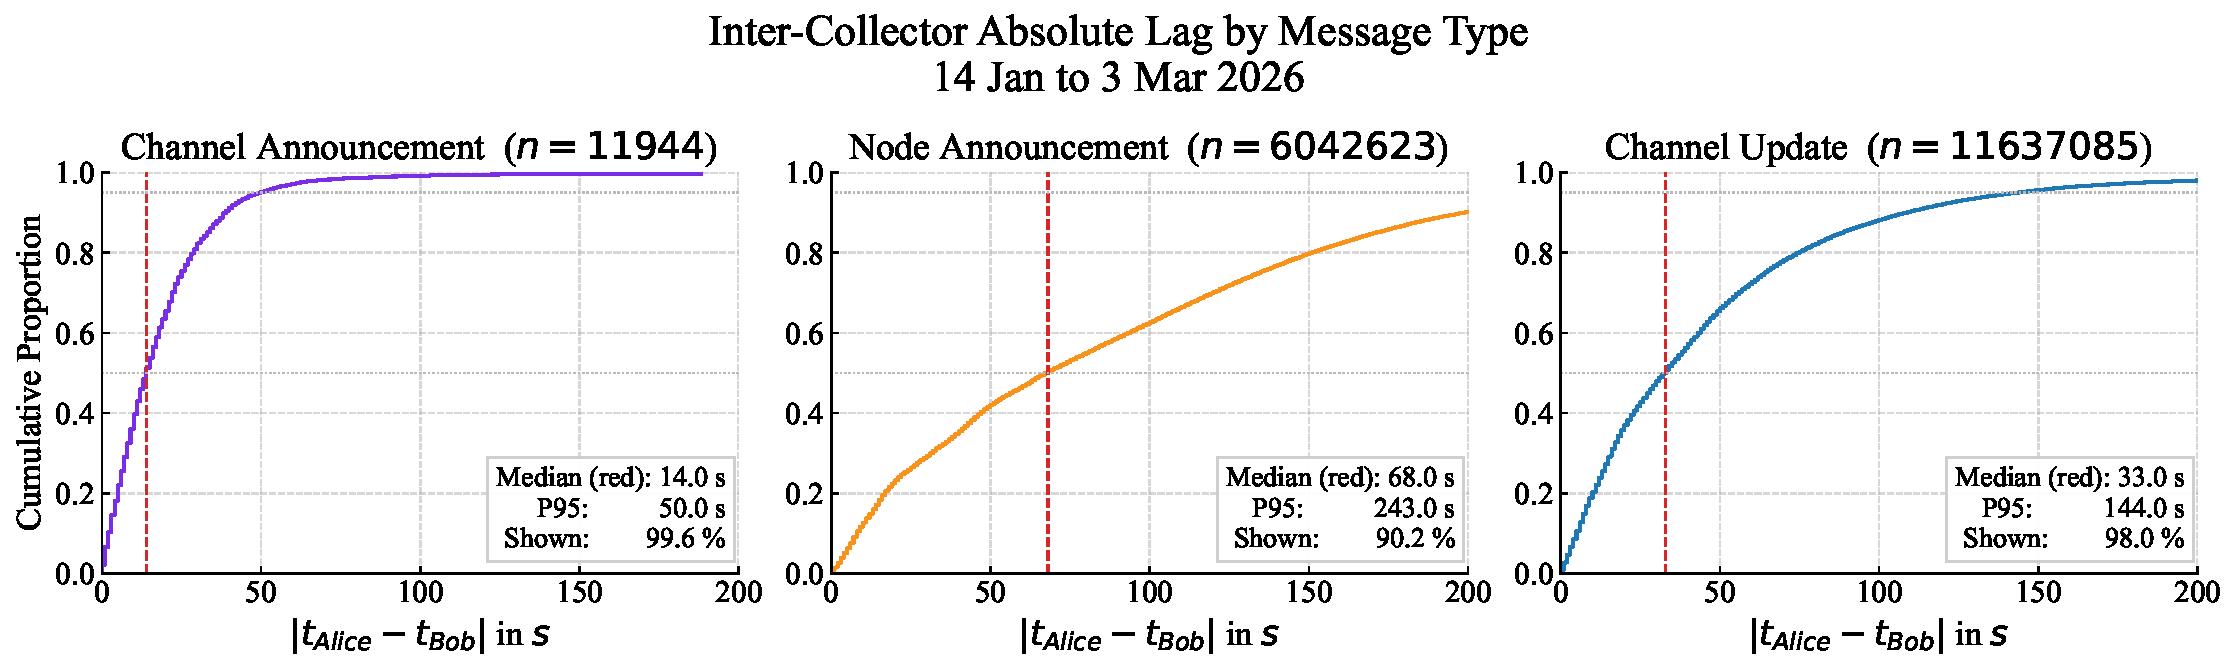
\includegraphics[width=\textwidth]{resources/results-final/inter-collector-lag-large.pdf}
    \caption{
        Distribution of the absolute inter-collection lag between the two collector nodes, 
        categorized by gossip message type.
        Two \gls{cln} nodes with the default configuration recieved 
        \code{channel\_announcements} closely with only \qty{14}{\second} difference.
        Further \code{node\_announcement} messages on median have a bigger variation of over a minute (\qty{68}{\second}).
        \code{Channel\_updates} lay in between with an absolute difference of \qty{33}{\second}
        The resolution is scaled to one second.
    }
    \label{fig:inter-collection-lag}
\end{figure}

To ensure the integrity of the measurement, extreme anomalies caused by a collector crash
were removed to isolate the steady-state network behaviour. 
The resulting distribution is shown in \autoref{fig:inter-collection-lag}.

An interesting observation is the steepness with which the \gls{cdf} curves drop, 
highlighting a generally high degree of synchronization between the two collector nodes. 
However, the exact synchronization speed varies significantly depending on the message type.

The \code{node\_announcements} on the other hand get received at much different times.
As they do not have an immediate effect on payment routing, this is not worrying.

Every channel must have at least one \code{channel\_update} message referenced to it,
so that the routing policy are met during payment routing.
The fact that it takes only $33 s$ on median per \code{channel\_udpate} message,
shows that they propagate much quicker.

\code{Channel\_announcement} messages are synchronized tightly, 
with a median inter-collection lag of only \qty{14}{\second}. 
Furthermore, the \num{95}th percentile is reached at just \qty{50}{\second}. 
This indicates that once a new channel is propagated the parallel network paths ensure 
both nodes discover it almost simultaneously.

Similarly, \code{channel\_update} messages are synchronized quickly, 
with a median absolute difference of \qty{33}{\second}. 
Because every active channel must maintain the latest routing policies to successfully route payments, 
the \gls{ln} focuses on rapid synchronization of these updates. 

On the other hand, \code{node\_announcement} messages exhibit a much wider variance, 
with a median lag of \qty{68}{\second}. 
Because these messages function primarily as informational heartbeats and do not have an immediate impact on payment routing, 
they are not as prioritized as the other two message types.


\subsection{Peer Session Analysis}
\label{sec:peer-session}

Empirical research regarding the long-term peer management behaviour of Lightning Network nodes (specifically \gls{cln} implementation) is rare.
Because the gossip protocol relies on active \gls{p2p} connections to propagate messages, understanding the connection stability is important. 
Utilizing the \service{peer-manager} component, the \tech{ln-history} platform continuously logged the lifecycle of all peer sessions established by 
our two collector nodes (\textit{Alice} and \textit{Bob}).

In this section we first show the distribution of peer session durations.
Next, we investigate whether a correlation exists between a peer's node size and its connection stability.

\subsubsection{Peer Session Distribution}
For the \gls{ln} to work, it is necessary that nodes receive gossip messages, but
there is no enforcement for nodes to send it.
As the collector nodes do not maintain any channels, some peers do not see a reason
to share their gossip to them, since they do not need it as they cannot route payments.

\begin{figure}[htbp]
    \centering
    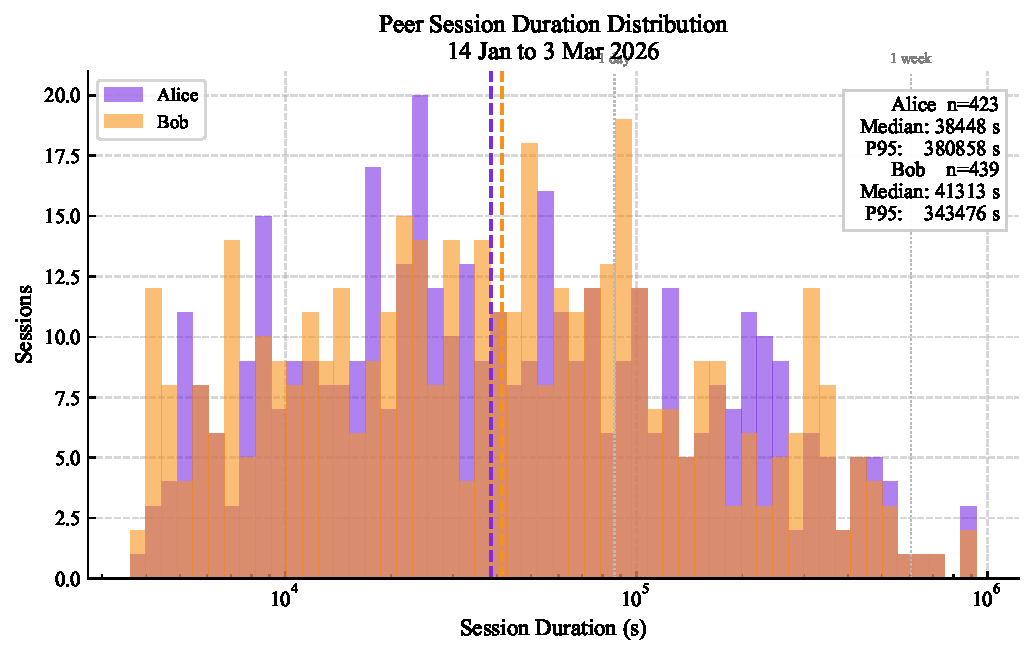
\includegraphics[width=0.7\textwidth]{resources/results-final/peer-session-distribution.pdf}
    \caption{
        Distribution of peer sessions with the collector nodes (\textit{Alice} and \textit{Bob}) 
        show that they have roughly the same number of connections ($423$ and $439$) in the time frame.
        The session durations vary a lot but have approximately the same median at around 11 hours.
    }
    \label{fig:peer-session-distribution}
\end{figure}

The \autoref{fig:peer-session-distribution} shows that the duration of peer
sessions varies between $30 min$ to up to over a week with a median at
$10.7 h$, $11.5 h$ for respectively \textit{Alice}, \textit{Bob}.


\subsubsection{Correlation between Peer Session Duration and Node Size}
Depending on the operational goals of a \gls{ln} node, 
actively selecting reliable peers for gossip propagation is advantageous. 

A sustained, uninterrupted \gls{p2p} connection implicitly indicates that the peer possesses 
a stable internet connection and robust underlying hardware. 

Therefore, we use the session duration as a proxy metric for the infrastructure reliability of the peer node.

\begin{figure}[htbp]
    \centering
    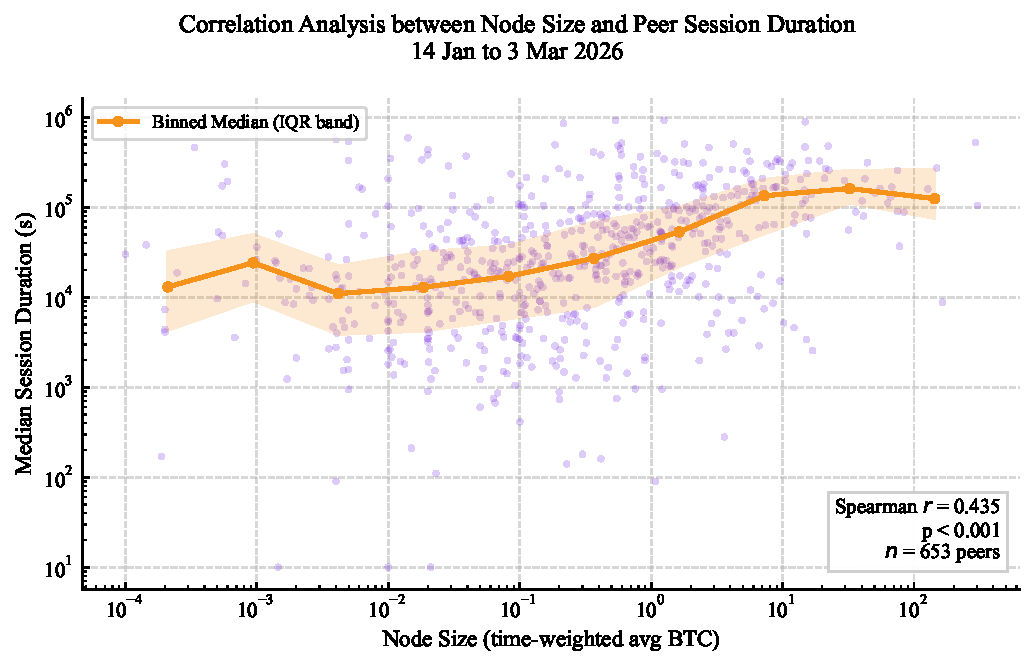
\includegraphics[width=0.7\textwidth]{resources/results-final/corelation-node-size-and-session-duration.pdf}
    \caption{
        A trend exists that larger nodes tend to support longer sessions with a 
        correlation coefficient $r = 0.435$ (statistical significance $p < 0.001$).
        The node sizes indicated as purple dots are binned into \num{10} bins. t
        The orange dots represent their median and the area around the graph shows 
        the 25th and 75th percentile of each bin.
    }
    \label{fig:peer-session-correlation}
\end{figure}

The \autoref{fig:peer-session-correlation} shows a moderate but positive correlation 
(Pearson's $r = 0.435$, $p < 0.001$) between the node size and the session duration. 
This trend suggests that highly capitalized routing nodes are generally operated 
on professional (high-availability) infrastructure, leading to fewer connection drops.

For node operators, this finding offers a strategy to mitigate the gossip synchronization blind spots
which were shown in \autoref{fig:network-gossip-volume-and-overlap}.
\\


\section{Historic Gossip Analysis}
\label{sec:historic-gossip-analysis}

This section analyses the complete set of public gossip messages collected between 2018 and April 2026
and persisted in the \tech{ln-history} platform, which in total are approximately \num{91.3} million.


\subsection{Gossip Distribution}

To establish a foundational understanding of the dataset, we first examine the historic distribution of gossip messages categorized by their respective types. 
After that, we utilize the \service{ln-history-api} to generate snapshots of the network graph, allowing us to analyse topology changes over time.
 
As defined in the BOLT specifications, \code{node\_announcement} and \code{channel\_update} messages have a \code{timestamp} field. 
Because \code{channel\_announcement} messages lack this field, we utilize the \code{funding\_timestamp} 
which is the confirmation time of the underlying funding transaction. 
Aggregating these timestamps allows us to visualize the monthly volume of the entire dataset.


\begin{figure}[H]
    \centering
    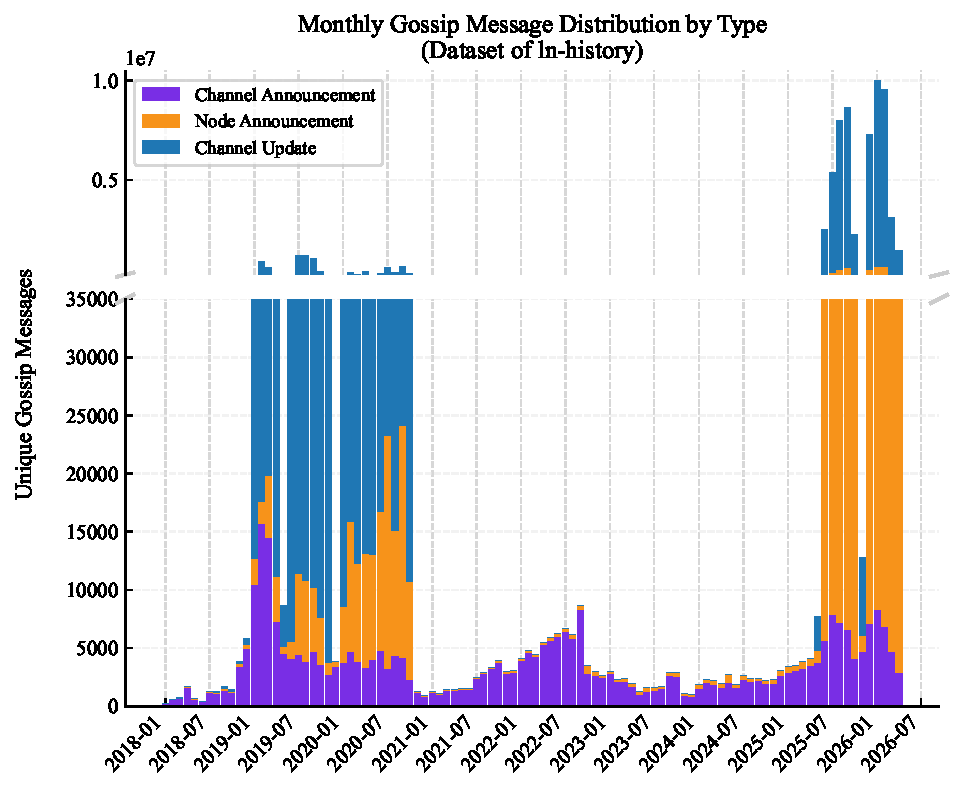
\includegraphics[width=0.7\textwidth]{resources/results-final/gossip-distribution-by-type.pdf}
    \caption{
        Monthly distribution of collected gossip messages by type. 
        The timeline highlights two distinct periods of intensive data archiving: 
        The initial 2019-2021 dataset provided by \citeauthor{decker_lnresearch_2020}~\cite{decker_lnresearch_2020}, 
        and the ongoing \tech{ln-history} collection beginning in mid-2025. 
    }
    \label{fig:gossip-messages-distribution}
\end{figure}

\autoref{fig:gossip-messages-distribution} provides insight into both the composition of the gossip messages and the share of the preserved data. 
Under active monitoring conditions, \code{channel\_updates} constitute the vast majority of all broadcasted messages, 
followed by \code{node\_announcements}, while structural \code{channel\_announcements} 
represent the smallest fraction of total traffic. 

Furthermore, the timeline illustrates two distinct periods of intensive data collection. 
The initial continuous block (from 2019 to roughly 2021) represents the invaluable open-source dataset 
aggregated by \citeauthor{decker_lnresearch_2020}~\cite{decker_lnresearch_2020}. 
Unfortunately, active support for that specific public archive ceased and 
the dataset exhibits a gap where mainly structural \code{channel\_announcements} were reliably preserved.

The second spike of data represents the active operation of the \tech{ln-history} platform, 
which successfully bridges this historical data gap and ensures continuous, future-proof data collection. 

Beyond the collection mechanics, the data shows a trend that the overall volume of gossip 
network traffic has increased significantly as the \gls{ln} has grown.


\subsection{Channels}

Payment channels are the foundational scaling mechanism of the \gls{ln}. 
In this section, we analyse the operational lifetime of these channels and investigate 
whether a correlation exists between a channel's lifetime and its committed capacity.

\subsubsection{Distribution of Channel Lifetime}

The lifespan of a channel is limited by two on-chain events: 
its creation via a funding transaction, and its termination when the underlying funding \gls{utxo} is 
spent\footnote{Recent protocol advancements, such as \term{channel splicing}, allow a funding \gls{utxo} 
to be spent to resize a channel's capacity without disrupting its operational continuity from the user's perspective. 
However, for the historical topological analysis, any on-chain spending of the original funding \gls{utxo} is considered as a channel closure.}. 
By measuring the time difference between these two block timestamps, we can calculate the lifetime of every closed channel in our dataset.

\begin{figure}[htbp]
    \centering
    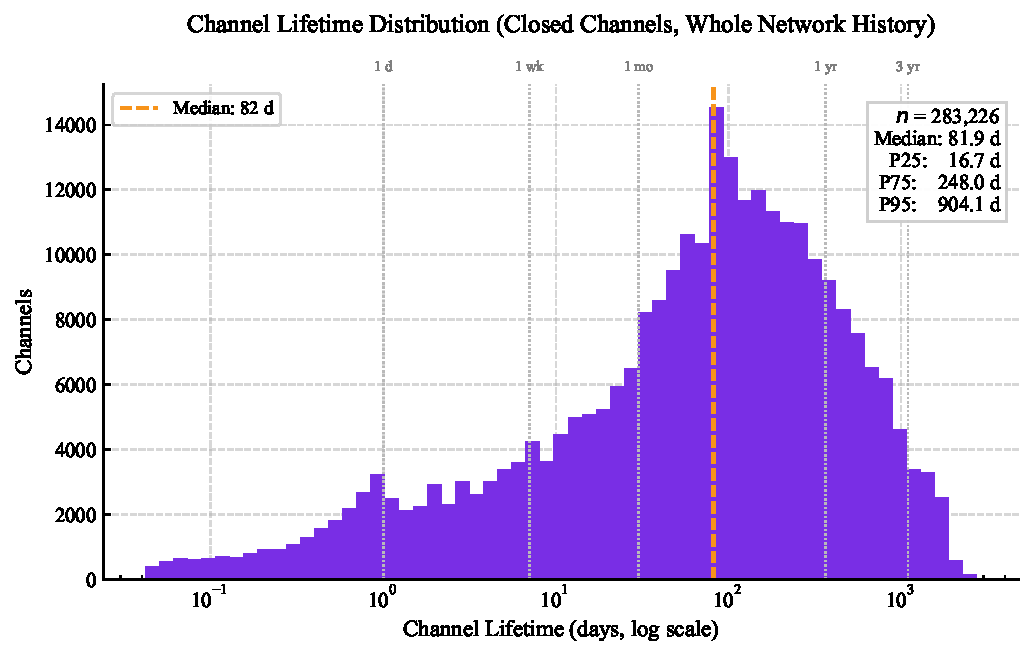
\includegraphics[width=0.7\textwidth]{resources/results-final/channel-lifetime-distribution.pdf}
    \caption{
        The median channel lifetime distribution of closed channels is \qty{105.6}{\day} days with a large variance.
        Some channels only exist for a few days whereas others survived multiple years. 
    }
    \label{fig:channel-lifetime-distribution}
\end{figure}


As shown in \autoref{fig:channel-lifetime-distribution}, the lifespan of \gls{ln} channels has a large variance. 
The median channel lifetime is \qty{81.9}{\day} (approximately three and a half months). 


On the one hand the distribution's long tail proves that stable channels surviving for multiple years do exist, 
but on the other hand the empirical data reveals a different reality for the majority of the network.

A significant concentration of channels exists at the extreme lower bound of the distribution, 
indicating that a substantial portion of channels are closed within just a few days of their creation.

It is important to note that this specific metric suffers from \textit{survivorship bias}. 
The calculation exclusively evaluates closed channels and therefore systematically excludes the network's 
long-living active channels that remain operational as of writing. 
We can therefore say that the true median lifetime of all successfully established \gls{ln} channels is likely
higher than what this subset suggests.


\subsubsection{Correlation between Channel Size and Channel Lifetime}

Because opening and closing channels costs on-chain Bitcoin mining fees, 
it is economically advantageous for node operators to maintain open channels for as long as possible. 
As established in \autoref{sec:peer-session}, well-capitalized node operators tend to have better infrastructure, 
resulting in higher reliability and longer peer sessions. 

A natural extension of this observation is to guess whether this operational professionalism translates to channel management. 
We investigate whether channels with higher capacity exhibit longer operational 
lifespans than smaller, potentially hobbyist-run channels.

\begin{figure}[htbp]
    \centering
    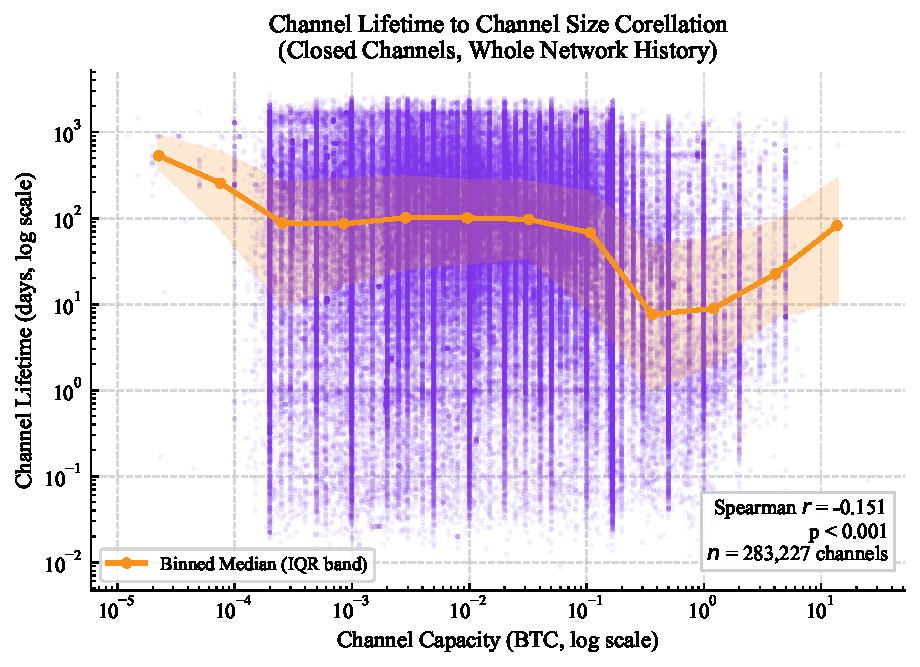
\includegraphics[width=0.7\textwidth]{resources/results-final/channel-capacity-lifetime-correlation.pdf}
    \caption{
        Scatter plot evaluating the relationship between a channel's capacity and its operational lifetime. 
        The data indicates no statistically significant correlation between the two variables.
    }
    \label{fig:channel-lifetime-correlation}
\end{figure}

Surprisingly, as illustrated in \autoref{fig:channel-lifetime-correlation}, 
the empirical data reveals absolutely no correlation between the channel capacity and its lifetime. 
It appears that channels are opened and closed at similar frequencies entirely independent of their capacity. 

This behaviour is likely compounded by the conditions of the Bitcoin mining fees. 
For the vast majority of the analysed timeframe, on-chain transaction fees remained low. 
When base-layer settlement costs are negligible, the financial penalty for closing and reopening channels is reduced, 
Therefore, closures are more likely dictated by other factors, like liquidity imbalances or active capital reallocation, 
which affect channels of all sizes.



\subsection{Centrality}
\label{sec:centrality}

This final section of the analysis chapter showcases how the snapshot generation 
of the \service{ln-history-api} can be used for in depth analysis of the topology of the \gls{ln}.

While graph centrality can be evaluated using a variety of metrics,
the main function of the \gls{ln} is payment routing.
The payment routing algorithms implemented by Lightning node clients use 
variations of Dijkstra's shortest-path algorithm~\cite{saraswathi_exposition_2024}.
This led to the selection of \gls{bc}. 
As defined by \citeauthor{newman2018networks}~\cite{newman2018networks}, 
\gls{bc} ranks each node based on the exact frequency of its occurrence along 
the shortest paths calculated between all possible node pairs in the network.


\subsubsection{Betweenness Centrality Concentration (Gini Coefficient)}

The Gini coefficient is a standard statistical metric used to quantify inequality within a distribution.
It is a number between \num{0} (perfect equality) and \num{1} (maximal inequality)~\cite{gini_variabilita_1912}. 

Applying the Gini coefficient to \gls{bc} to evaluate \gls{ln} centralization was first 
done by \citeauthor{zabka_short_2022} in \citetitle{zabka_short_2022}~\cite{zabka_short_2022}. 

In this section, we expand upon their foundational research. 
By utilizing the highly optimized snapshot creation of the \tech{ln-history} platform, 
we are able to compute these complex centrality metrics across a significantly higher temporal resolution 
and over a substantially extended historical time horizon.

\begin{figure}[htbp]
    \centering
    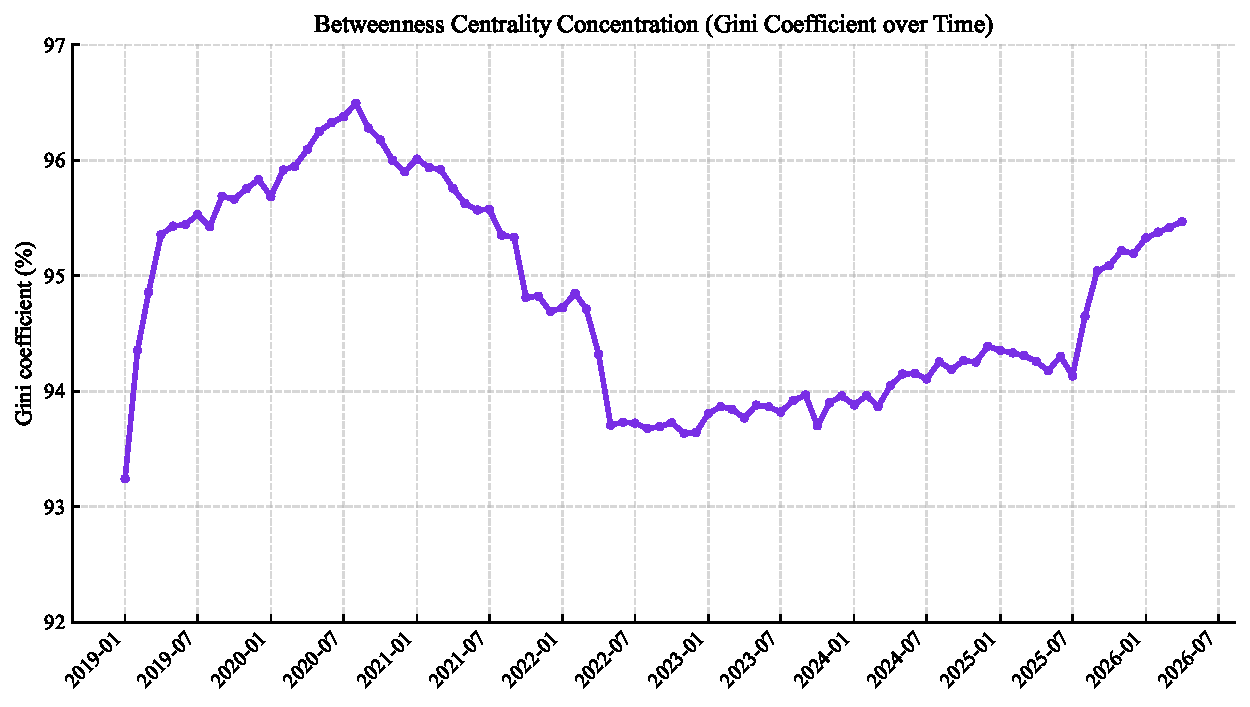
\includegraphics[width=\textwidth]{resources/results-final/centrality-gini.pdf}
    \caption{
        Gini coefficient of the \gls{bc} across network snapshots from 2018 to 2016, 
        With values abolve \qty{90}{\percent} the centrality of the \gls{ln} is high and has remained high.
    }
    \label{fig:betweenness-centrality-gini}
\end{figure}

As illustrated in \autoref{fig:betweenness-centrality-gini}, the Gini coefficient has remained high
with fluctuating values between \qty{93}{\percent} and \qty{97}{\percent}.

This result shows that almost every two pair of nodes when connected with the shortest path,
needs to route through the same few central nodes.

The implications of this topology will be discussed in the \autoref{ch:conclusion}.


\subsubsection{Betweenness Concentration by Top Percentiles over Time}
To further investigate this structural inequality, we categorize the routing nodes 
into percentiles based on their proportional share of the total network \gls{bc} over time.
\begin{figure}[htbp]
    \centering
    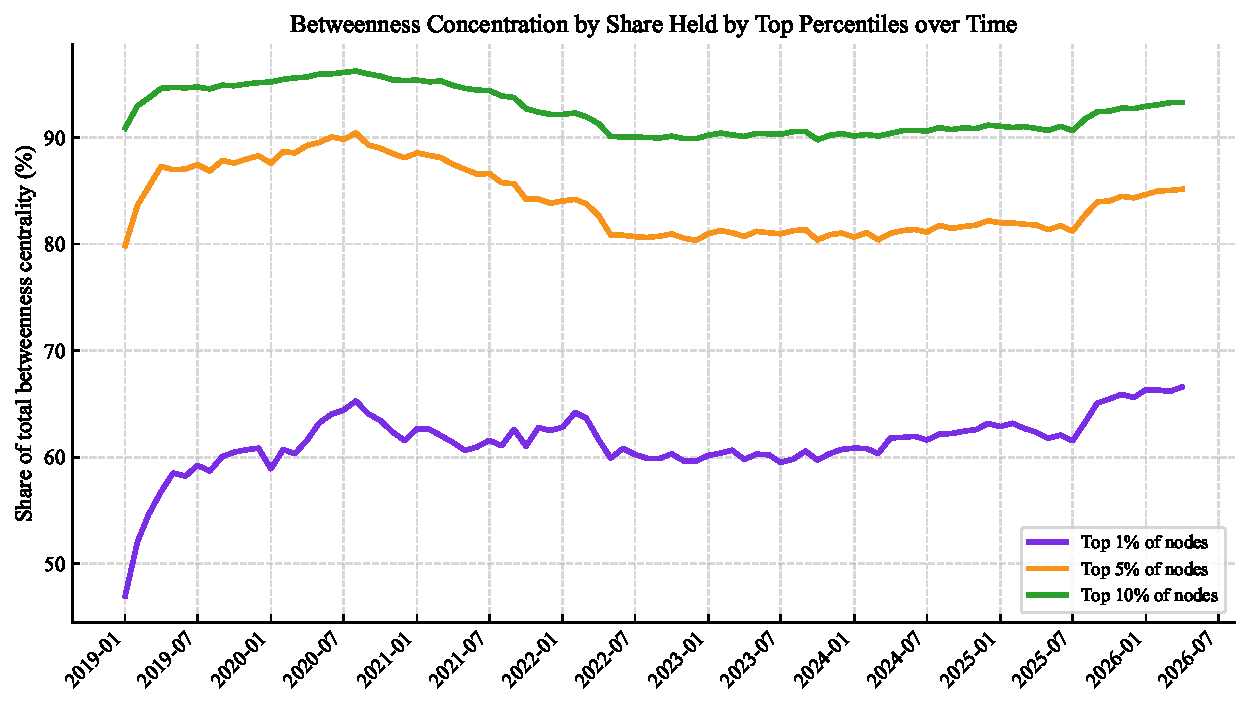
\includegraphics[width=\textwidth]{resources/results-final/centrality-concentration-top-percentiles.pdf}
    \caption{
        Since the beginning of the \gls{ln} the top \qty{1}{\percent} of nodes
        own more than \qty{50}{\percent} of the share of total \gls{bc}.
        Further, the top \qty{10}{\percent} around \qty{90}{\percent}.
    }
    \label{fig:betweenness-centrality-top-percentiles}
\end{figure}

The \autoref{fig:betweenness-centrality-top-percentiles} underlines the previous analysis 
that the \gls{ln} is centralized with only a few nodes having an enormous share of total \gls{bc}.
The top $10 \%$ of nodes posses over $90 \%$ of the total \gls{bc}.


\iffalse
\subsubsection{Lorenz Curve Evolution}
\begin{figure}[htbp]
    \centering
    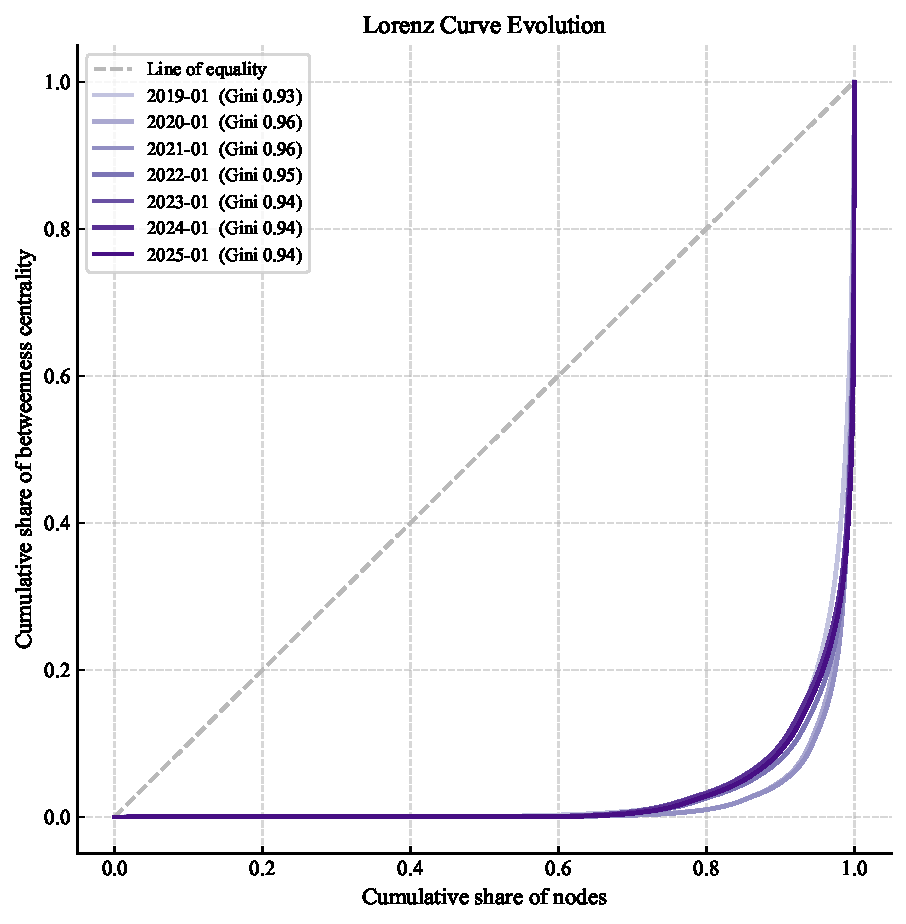
\includegraphics[width=\textwidth]{resources/results-final/lorenz-curve.pdf}
    \caption{
        Lorenz Cureve
    }
    \label{fig:lorenz-curve}
\end{figure}
\fi


\subsubsection{Heatmap of Top Nodes by Betweenness Centrality over Time}

To conclude this topological analysis, we determine the \gls{ln} most influential routing hubs.

We can name the exact nodes that have major influence in the \gls{ln}.
Over its lifetime of the \gls{ln} they have established themselves as important hubs.

By tracking the \gls{bc} rankings of individual nodes across the historical snapshots, 
we visualize the network's central hubs in a heatmap.

\begin{figure}[htbp]
    \centering
    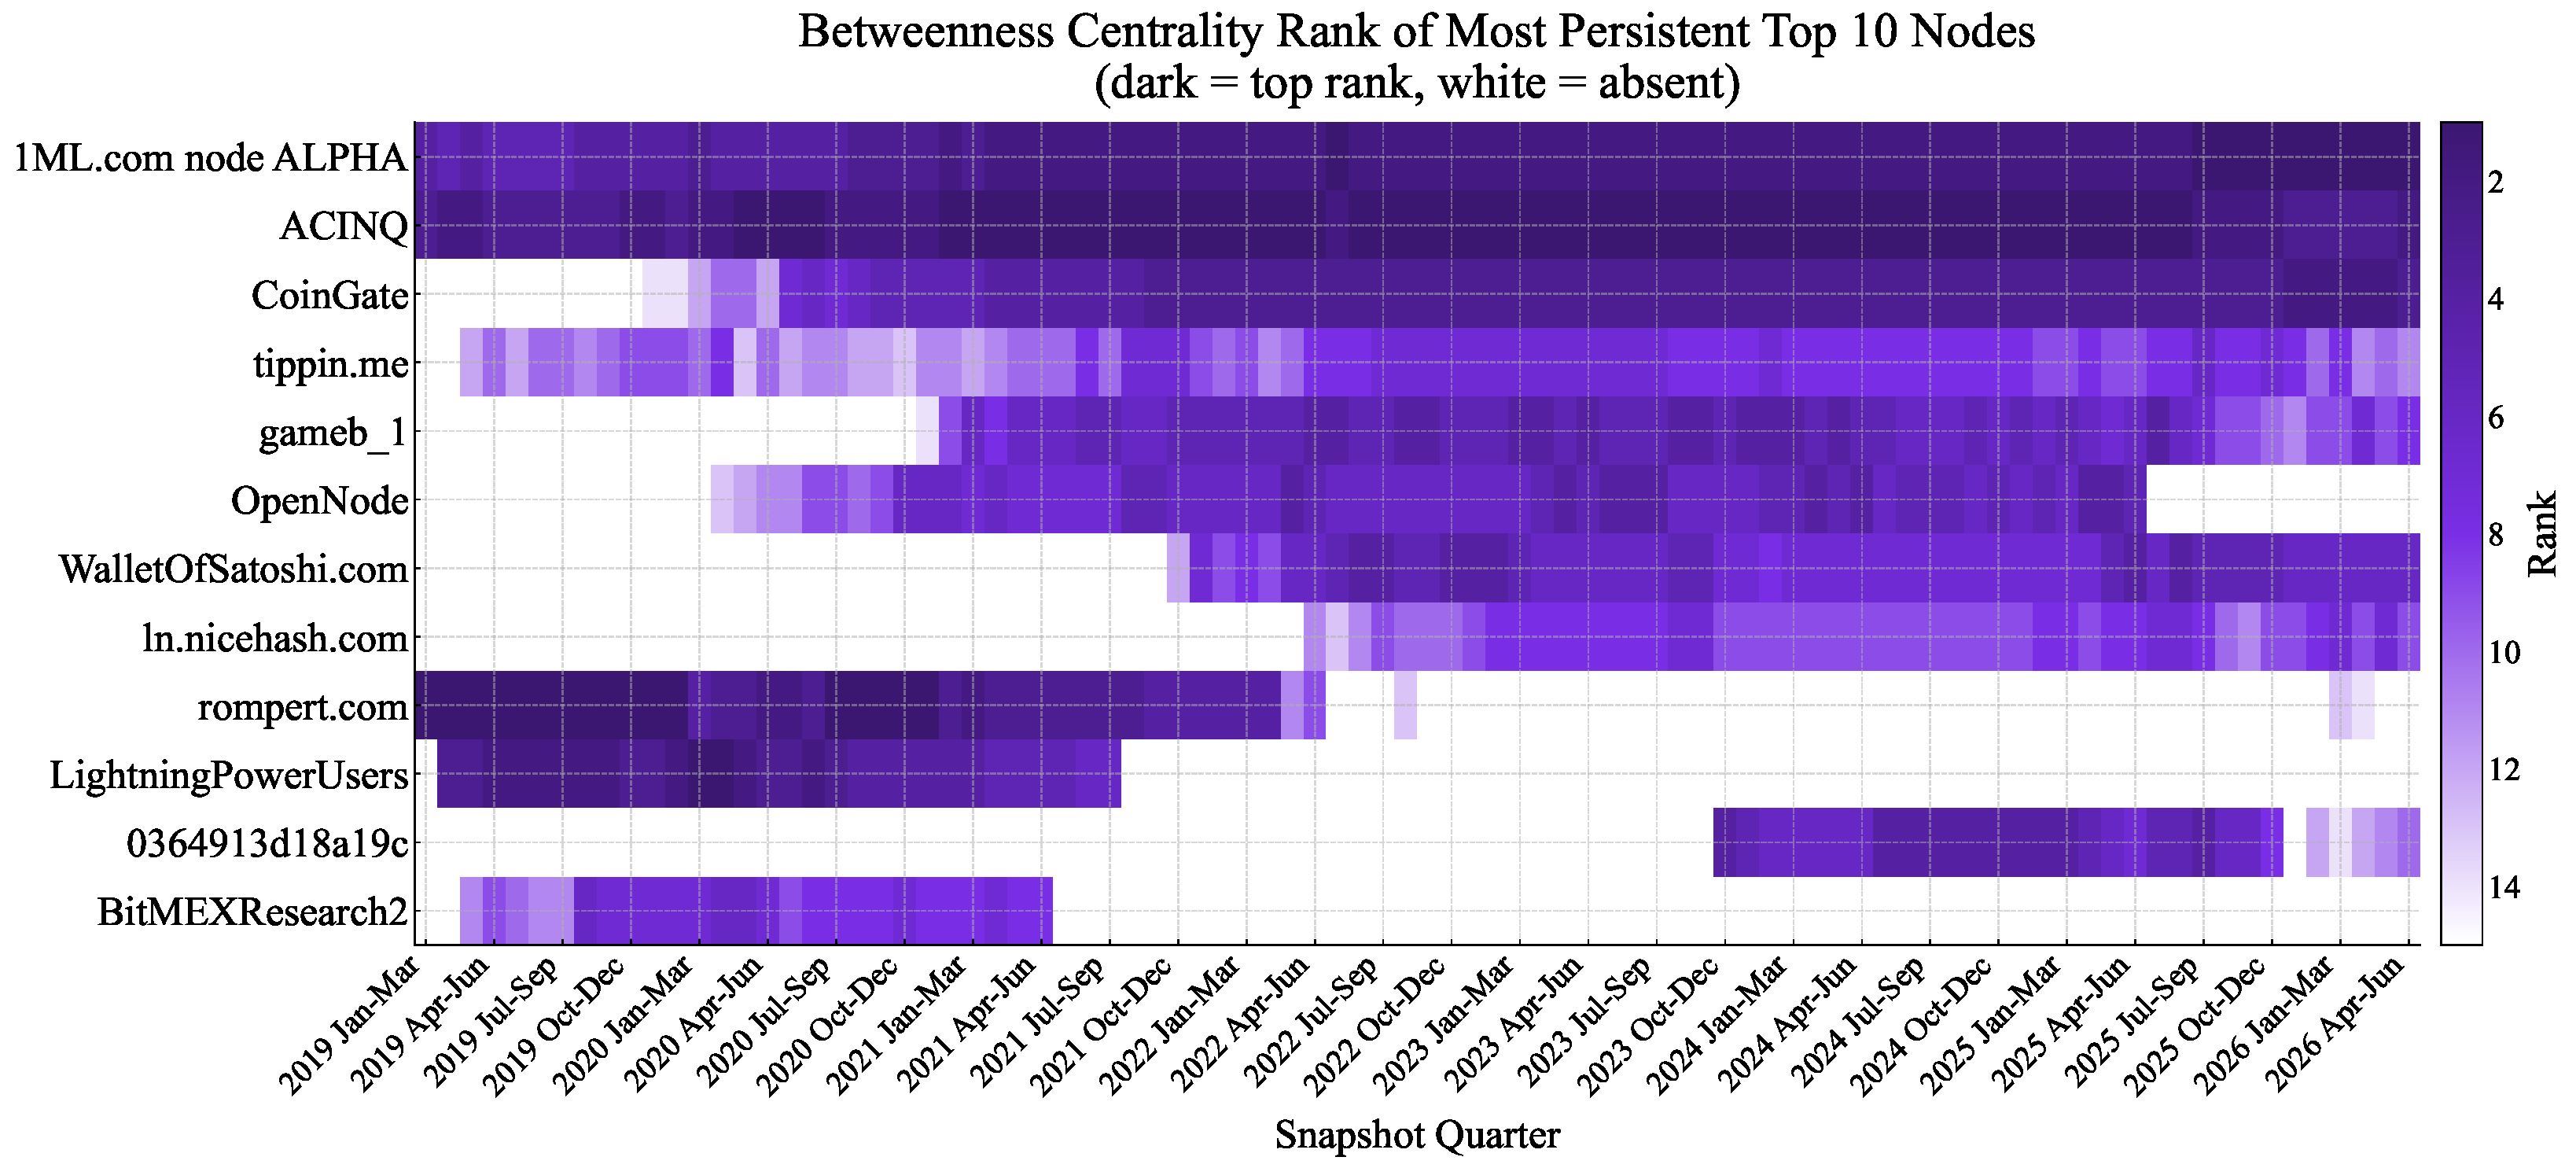
\includegraphics[width=\textwidth]{resources/results-final/centrality-top-nodes-heatmap.pdf}
    \caption{
        Heatmap tracking the betweenness centrality rankings of the most 
        central nodes across the whole history of the \gls{ln}.
    }
    \label{fig:top-nodes-heatmap}
\end{figure}

The \autoref{fig:top-nodes-heatmap} visualizes how a few nodes namely 
\textit{ACINQ}, \textit{1ML} and \textit{CoinGate} have dominated and still dominate
the network when looking at betweenness centrality ranking of the \gls{ln}.

We discuss the consequences of this in \autoref{ch:conclusion}.

\iffalse
Future ideas:

\item 4B Tor vs clearnet share of nodes per snapshot for every quarter of existing gossip

SUB Gossip analysis: which nodes send which gossip (redundant or actualy new information)
\item 1D Bigger nodes update more frequently, correlation?
\item 1E Bigger channels update more frequently?
\item 1F Looking at a channel: Does the bigger or smaller node update the fees more often?

\item 1G Distribution how many channel_update messages are actually new and which are redundant
\item 1H Divide the network into active and passive nodes based on channel_update msg
\fi
	\chapter{Conclusion}
\label{ch:conclusion}

The conclusion is divided into three sections and summarizes the core findings of this thesis.
In \autoref{sec:platform-performance}, we assess the performance of the \tech{ln-history} platform,
specifically how well the platform architecture met its requirements in a production environment and how to improve it.

After that we delve into a discussion about the meaning of the analysis.
\autoref{sec:ln-gossip-protocol-conclusion} presents a conclusion about the \autoref{sec:metadata-analysis}.
Likewise, the \autoref{sec:ln-evolution} concludes the \autoref{sec:historic-gossip-analysis}.


\section{\tech{ln-history} Platform Performance}
\label{sec:platform-performance} 

The evaluation of the platform's functional and non-functional requirements demonstrates
that the \tech{ln-history} architecture is capable of supporting advanced, empirical network research.

Through its custom data model, the platform manages long-term data storage and persistence (\ref{req:persistance}), 
alongside fulfilling the dual-format constraint for preserving both raw wire bytes and parsed data (\ref{req:dual-format}). 

For historical analysis, the system achieves snapshot retrieval (\ref{req:snapshot}) times averaging under \qty{3}{\second}.
However, we observed that while database retrieval is exceptionally fast, 
the resulting payload for a modern network snapshot still requires approximately \qty{50}{\mega\byte}. 
Consequently, network bandwidth and not the database performance remains 
the primary temporal bottleneck for end-users executing these queries.

In terms of real-time operations, the platform demonstrated reliability, 
running stably without major outages throughout the 48-day collection window. 
The real-time ingestion pipeline successfully processed multiple gigabytes of gossip messages (\ref{req:ingestion}), 
consistently maintaining an ingestion lag of under \qty{5}{\minute} under normal network conditions
without blocking parallel analytical queries (\ref{req:concurrency}). 

Meeting the non-functional requirements self-hostability (\ref{req:self-host}) and 
long-term maintainability (\ref{req:maintainability}) proved more challenging. 
While the system can operate on small-scale hardware, processing heavy \gls{olap} queries and 
bulk ingestions pushed the server to its thermal limits.

Maintaining optimal query performance requires active administration.
The commands \code{ANALYZE VACUUM FULL} and \code{CLUSTER} are necessary to prevent index degradation over time. 
Those challenges lead to the decision to migrate the database to a dedicated datacenter \gls{vps} 
ensuring the reliability required for the empirical analysis in this thesis.


\section{Lightning Network Gossip Protocol}
\label{sec:ln-gossip-protocol-conclusion}


\subsection{Network Gossip Volume and Lag}

As \autoref{sec:metadata-analysis} shows, Lightning nodes do not inherently have a 
correctly synchronized or complete view of the network topology. 
Beyond that, the protocol has disparities in propagation latency depending on the message type. 
During data cleaning, more than half of the collected \code{node\_announcements} 
were broadcasted redundantly without containing any novel topological information. 
Given the propagation blind spots, the inherent latency variations, and the overhead of redundant metadata, 
the empirical analysis shows that researching and implementing optimizations to the gossip protocol is necessary for long-term scalability. 
Various approaches to address these architectural bottlenecks will be discussed in the upcoming \autoref{ch:future-work}.


\subsection{Peer Session Analysis}

This thesis contributes empirical observations regarding the peer management behaviour of default \gls{cln} nodes. 
While the \gls{ln} operates without an enforcement to forward gossip messages, 
active participation in the gossip protocol fundamentally relies on stable \gls{p2p} connections. 
The analysis demonstrated that peer session durations have an immense variance, ranging from minutes to multiple days. 
When coupled with the synchronization inaccuracies discussed previously, 
the connection instability can yield to missing gossip messages.

Nodes that offer routing services are economically incentivized to maintain highly reliable peer connections,
a dynamic empirically supported by our finding that total node capacity positively correlates with the session duration. 
By ensuring uninterrupted access to gossip messages, specifically \code{channel\_updates},
these enterprise-level hubs can minimize payment routing failures and optimize their overall service reliability.
Smaller nodes that have an unstable connection are more prone to payment failures. 
By missing critical \code{channel\_updates} during periods of downtime, 
these nodes risk to use outdated fee policies and inaccurate topological data during their pathfinding calculations.



\section{Lightning Network Evolution}
\label{sec:ln-evolution}

The evolution of the \gls{ln} is a complex topic and can be viewed from different angles.
As we will see, the network has grown and matured in the past eight years.
Nonetheless, there are still many open questions and possible improvements to be made.

Following the structure of the \autoref{sec:historic-gossip-analysis}, 
we first discuss the quality of the gossip dataset currently persisted in the \tech{ln-history} platform.
After that we will examine empirical measurements of all observed closed channels.
Lastly, we will dive into discussions about the centrality of the \gls{ln}.


\subsection{Collected Gossip Messages}

As mentioned in \autoref{sec:historic-gossip-analysis}, evaluating the complete 
repository of over \num{91.3} million historical gossip messages 
reveals two distinct phases of intensive data collection, 
separated by a multi-year observational blind spot between 2022 and mid-2025. 
Despite this gap in ephemeral \code{channel\_updates}, 
the structural integrity of the historical network graph can be approximated reconstructed 
because the foundational \code{channel\_announcements} were largely preserved. 
Furthermore, the \autoref{fig:gossip-messages-distribution} shows a hierarchy in network traffic composition. 
Dynamic \code{channel\_updates} dominate the broadcast volume, followed by informational \code{node\_announcements}, 
while structural \code{channel\_announcements} represent only a tiny fraction of the gossip protocol.


\subsection{Channels}

Payment channels form the core of the \gls{ln} protocol. 
In this section, we discuss the empirical findings of over \num{283226} closed channels.
The theoretical objective of a payment channel is to remain open indefinitely, 
allowing nodes to route an unlimited number of off-chain transactions while 
amortizing the initial on-chain setup fees. 
However, as \autoref{fig:channel-lifetime-distribution} illustrates, 
the empirical reality is different: of all channels that have ever been funded, 
more than \qty{75}{\percent} have been closed.

It is reasonable to assume that larger channels might have a longer lifespan than smaller ones. 
Node operators committing significant capital to open large channels 
likely plan their network topology more carefully. 
To test this hypothesis, we measured the correlation between channel capacity (\code{capacity\_sat}) 
and channel lifetime (\autoref{fig:channel-lifetime-correlation}).
Surprisingly, the data reveals no correlation between these two variables. 
A channel's financial size does not predict how long it will remain open.

Another interesting observation shows the scatter plot. 
Channel capacities with round numbers (e.g., \code{capacity\_sat} ending in $00000$) appear more often (see: purple vertical lines). 
This clustering indicates that funding amounts are rarely mathematically optimized for exact routing needs. 
Instead, they are often chosen based on human intuition or simple convenience.

Ultimately, channel management proves to be far more complex than 
simply opening a connection and leaving it alone. 
The lack of correlation to capacity shows that channels frequently require active adjustments, closures, and rebalancing. 
This reality affects all participants, regardless of whether they are a professional hub or an individual hobbyist.


\subsection{Centrality}

The academic discourse surrounding centrality in the \gls{ln} is extensive, 
compared to other research areas of the \gls{ln} protocol. 
Numerous studies have applied a wide range of graph-theoretic metrics 
to historic snapshots to quantify the network's topology (e.g., \cite{atmanaviciute_quantitative_2025}). 
The empirical data presented in \autoref{sec:centrality} aligns with this literature, 
confirming that the network is highly centralized according to \gls{bc}.

This thesis argues that the academic narrative is often one-sided. 
Applying centrality metrics to static snapshots to condemn the network for deviating from Bitcoin's decentralized ethos,
fails to critically evaluate the resulting operational value that dominant nodes provide.
From an economic and operational perspective, a centralized topology is a logical and arguably beneficial development. 
Professional routing hubs provide liquidity and continuous uptime necessary for a functional payment network. 
The presence of these dedicated backbone nodes is likely a driver behind the 
high payment success rates and overall service reliability that the \gls{ln} currently provides~\cite{random__reran_2024}.
Enforcing strict, uniform decentralization would likely increase routing failures.

Nonetheless, from the perspectives of privacy, censorship resistance, and systemic independence, 
this centralization of routing power definitely remains concerning. 
Relying on a handful of dominant hub operators contradicts the \gls{p2p} ethos of Bitcoin. 
These central hubs represent a significant vulnerability regarding user privacy. 
While Lightning payments utilize onion routing, central hubs process such a massive share of the total traffic 
that they are uniquely positioned to perform traffic analysis. 
By monitoring the flow, timing, and channel balances of adjacent packets, 
dominant routing nodes could theoretically try to trace and deanonymize payment flows, 
severely degrading the privacy guarantees originally engineered into the protocol.

Ultimately, the centrality of the \gls{ln} represents compromise that distributed systems have to face by design. 
The network has organically gravitated toward a topology that sacrifices a degree of ideological decentralization and 
strict privacy to achieve the operational efficiency, liquidity, and reliability required for real-world adoption.

\iffalse
\subsection{Functional Requirements}

\subsubsection{Data Storage \& Persistence (RF 1 \& 2)}
Thanks to the database centric layout with its custom data model,
the first two functional requirements RF1 and RF2 are met.

\subsubsection{Querying \& Historic Analysis (RF 3 - 5)}
To make \gls{olap} queries a lot of index maintanance is necessary.
The storage used by indexes reaches about the storage of the actual data
but is necessary to provide in depth analysis.

\paragraph{Snapshot Retrieval RF3}
The thrid functional requirement (RF3) stating that the plaform is able to retrive 
historic snapshots has been met very well. 
The pure retrieval of gossip messages from the database 
taks on average less than $\qty{3}{s}$. 

As the database utilizses its \gls{ram} to keep data that is often requested \textit{warm},
snapshot queries for similar timestamp can yield results even quicker.
As the analysis has shown snapshots with thousands of nodes and edges take up space.
A snapshot of the current lightning network from the \tech{ln-history} plaform,
which already reduces the number of gossip messages drastically and sends them in raw bytes,
still needs aroude $\qty{50}{\mega B}$, which depending on the network bandwidth
takes significantly more time to download than the actual retrieval from storage.

This main feature is working \textit{lightning} fast and shows that the \tech{ln-history}
platform is a significant upgrade for researchers when analysing historic snapshots.

\paragraph{Time-Window Retrieval RF4}
The fourth functional requirement (RF4) initially sounds interesting and close by
the snapshot retrieval but at the time of writing this thesis there has not been
many analysis ideas been found. 
The queries are, depending on the length of the time window,
rapid fast but still there is no use case yet.

\paragraph{Entity Filtering RF5}
This requirement is fulfilled and used in multiple queries specifically analysis
over channels or nodes.


\subsubsection{Real-Time Operations RF6 - RF10}
As shown in the first part of the analysis \autoref{sec:metadata-analysis},
the \tech{ln-history} platform has been running stable between  
%START_DATETIME_STR = "2026-01-14T00:00:00Z"
%END_DATETIME_STR = "2026-03-03T00:00:00Z"
.
In that time it processed multiple $\qty{}{\giga B}$ of gossip messages and
was able to ingest them.


\paragraph{Low-Latency Ingestion RF6}
RF6 which requires the database to reflect the live state of the network
by quickly inserting new gossip is reached.
The database thanks to batching gossip messages into a database transactions,
the ingestion throughput is not a problem and the \service{ln-history-database}
is capable to ingestion an order of magnitude more messages per second as normally
occur in the \gls{ln}

\paragraph{Concurrency RF7}
This requirement is almost fully met. In phases of exceptionally high workloads
onto the database (e.g. generation of many snapshots or complex \gls{olap} queries)
the insertion almost stops and an ingestion lag builds up.
But under normal conditions, the lag remains below $\qty{10}{s}$.

\paragraph{Multiple nodes RF8}
As of writing this thesis only two nodes have been collecting gossip messages.
The platform was capable of managing those, it should be possible to scale to at least
five concurrent running nodes.

\paragraph{Metadata RF9}
Thanks to the introduction of the \code{gossip\_inventory} and \code{gossip\_observations}
every collected gossip message immediatly gets an unique identifier \code{gossip\_id}.
Together with the \code{collector\_node\_id}, makes every gossip message unique.
Since every recieved gossip message gets its timestamp appended to it, it is really
easy to do propergation lag analysis over the gossip dataset. 


\paragraph{Batch ingestion RF10}
This script is doing its job but needs refactoring, since its generally a manaul 
process occuring rarely we consider this circumstance as fine.
Nonetheless, batch ingestions require the \service{gossip-processor} to stop
otherwise the ingestion will (depending on the size) take multiple days.


\subsection{Non-Functional Requirements}
The Non-Functional Requirements were defined by the following paragraphs and 
have sometimes been more challenging to meet than the functional ones.

\paragraph{Transparency \& Auditability (Open Source) NF 1}
This requirement forces the \tech{ln-history} platform to be fully open source
making it possible for other researchers to verify the results.
It met, by the fact that the source code of each component is openly available
\footnote{See https://github.com/ln-history}.


\paragraph{Deployability (Containerization) NF 2}
Thanks to the usage of Docker every component is containerized and working as intended.

\paragraph{Efficiency (Self-Hostability) NF 3}
This requirement was by far the most difficult to meet. 
We own a small scale server with a five-threaded CPU and DDR5 \gls{ram} as well
as modern NVMe SSD storage.
Nonetheless, during high \gls{olap} queries or at startup, where large amount
of missing gossip messages were being analysed / ingested, the server got heated up.
Since the platform ran without major outtage for 48 consecutive days, we consider this
requirement met, although for doing the analysis in chapter \autoref{ch:empirical-data-analysis},
we moved the database to a VPS in a datacenter, which in comparision proved so much more reliability.


\paragraph{Maintainability (long-term) NF 4}
Although the architecture strongly follows the \textit{Seperation of Concerns} pattern,
having multiple (independent) services working together, the maintainability can still be challenging.
Different gossip formats require delicate handling as updating already inserted gossip messages can get really difficult.
Also changing the interface of one service can have devistating cascading effects,
where the other components in the processing pipeline crash.
During development those constaintraints often lead to hours or days of troubleshooting.

Also the \service{ln-history-database} needs regular active maintainance to provide the expected service.
Especially the indixes and what postgres thinks of them deviates over time.
Using \code{ANALYZE VACUUM FULL} is a must, as well as regular \code{CLUSTER} commands  
\fi
    \chapter{Future Work}
\label{ch:future-work}

This chapter outlines future directions for research and development 
based on the empirical findings of this thesis. 

Building upon the capabilities of the \tech{ln-history} platform demonstrated, 
we list numerous avenues for extending these in \autoref{sec:ln-history-project}.

Secondly, because the empirical data highlighted inefficiencies in the gossip protocol, 
\autoref{sec:ln-gossip-protocol} explores its ongoing development. 
It discusses the upcoming \term{Gossip v2} protocol updates, 
currently being drafted by \citeauthor{lightningdevelopers_bolts_2018}, 
as well as fundamentally new designs to share gossip messages,
aiming to resolve these existing propagation bottlenecks.

After that, \autoref{sec:the-role-of-ln} steps back to discuss the evolution of the Bitcoin scaling ecosystem.
The \gls{ln} was envisioned in the whitepaper \citetitle{poon_bitcoin_2016} as a decentralized, 
\gls{p2p} network capable of making Bitcoin a globally viable medium of exchange~\cite{poon_bitcoin_2016}. 
Nonetheless, as discussed in \autoref{ch:conclusion}, 
the network has matured with central hubs forming a backbone for payment routing.
To finish off, an outlook on emerging Layer-2 solutions that either complement the \gls{ln} or 
offer alternative approaches to scaling Bitcoin payments, is presented.


\section{\tech{ln-history} Project}
\label{sec:ln-history-project}

Because the \tech{ln-history} platform was designed with a modular architecture, 
it provides a foundation for extensive future development. 
These improvements can generally be categorized into expanding the platform's 
analytical capabilities and scaling its underlying infrastructure.

\paragraph{Analytical Extensions}

The dataset of \gls{ln} gossip messages and peer session metadata opens
many directions for future empirical research. 
The platform could be extended to track and analyse the following network statistics:

\begin{description}[leftmargin=1em, style=nextline]
    \item[Node Implementation Heuristics:] 
        By analysing the \term{feature-bits} within \code{node\_announcements}, 
        the platform could classify the network share of different Lightning node client software. 
        This could be achieved by natively integrating the scanning heuristics developed by 
        \citeauthor{myers_impscan_2025}~\cite{myers_impscan_2025} into the \service{gossip-processor}.
    
    \item[ISP and Cloud Centralization:] 
        Extending the peer address data model to resolve Autonomous System Numbers (ASNs) 
        and TLS certificates would allow researchers to quantify the network's reliance on major cloud providers, 
        similar to the analysis done by the \citetitle{mempooldevelopers_mempool_2026} project~\cite{mempooldevelopers_mempool_2026}.
    
    \item[Tor Network Dynamics:] 
        Deploying additional collector nodes operating only behind the Tor network 
        would enable comparative studies to measure whether privacy-preserving nodes 
        suffer from increased propagation lag or topological isolation compared to clear-net nodes.
    
    \item[Advanced Closure Analysis:] 
        Expanding the \code{channel\_closures} management (done by \service{chain-enricher}) 
        could provide deeper insights if channel closures are uni- or bilateral.
        Additionally, an analysis of spent mining fees for closures and 
        the final liquidity distribution of the closed channel could be made.
    
    \item[Negative Routing Fees:] 
        The database could be updated to track the addition of negative routing fees by the \citeauthor{lnddeveloper_lightningnetwork_2026}~\cite{lnddeveloper_lnd_2024}, 
        allowing researchers to analyse the effect onto the network and which nodes use them.
    
    \item[Routing Algorithm Simulations:] 
        The historical snapshots generated by the \service{ln-history-api} provide the perfect empirical foundation 
        for back-testing and evaluating the efficiency of (new) pathfinding algorithms on real-world topologies.
        Extending the research done by \citeauthor{saraswathi_exposition_2024} in~\cite{saraswathi_exposition_2024}.
    
    \item[Fee Market Correlations:] 
        Pending the recovery of the missing \code{channel\_update} data for the year 2024, 
        future research could investigate whether node operators dynamically adjust their routing fees
        in response to transaction fees in the Bitcoin blockchain.
\end{description}


\paragraph{Infrastructural Scaling}

Currently, the platform operates on a single virtual machine utilizing \tech{Docker Compose}. 
While this was a solid, resource-efficient decision for the scope of this thesis, 
the planned addition of new collector nodes and heavier analytical workloads will require more resources. 

To achieve true \term{high-availability} and manage growing data volumes, 
the infrastructure should be migrated to \tech{Kubernetes}~\cite{burns_borg_2016}. 
Adopting this industry standard for container orchestration would enable a new degree of scalability, 
allowing individual services such as the \service{gossip-processor} and \service{chain-enricher}
to be scaled horizontally across a distributed cluster based on real-time network traffic.


\section{Gossip Protocol}
\label{sec:ln-gossip-protocol}

This section examines two current developments for the \gls{ln} gossip protocol. 
First, we outline the \term{Gossip v2} architecture to support new channel types. 
Secondly, we discuss the potential integration of \term{set reconciliation technologies} 
to optimize bandwidth and propagation efficiency.


\paragraph{Gossip v2}
The activation of the Taproot soft fork introduced the cryptographic foundation for \term{Taproot channels}~\cite{wuille_bip341_2020}. 
Unlike \textit{legacy} channels that rely on visible 2-of-2 \gls{p2wsh} multisignature scripts, 
Taproot channels utilize Schnorr signatures~\cite{wuille_bip340_2020} and MuSig2 key aggregation~\cite{nick_musig2_2021}. 
This allows the channel funding transaction to appear identically to a standard, single-signature transaction on-chain, 
improving network privacy by making Lightning channels look like regular Bitcoin transactions.

The legacy gossip protocol v1 is structurally incompatible with these new cryptographic primitives.
The proposed \term{Gossip v2} (sometimes referred to as v1.5 or v1.75 during the development phases) 
introduces native support for Schnorr signatures. 
The specification draft has just been merged on May 4th 2026~\cite{mouton_extensionbolt_2023}.


\paragraph{Set Reconciliation and Minisketch}

As concluded in \autoref{ch:conclusion}, the current \gls{ln} gossip protocol suffers 
from bandwidth inefficiencies and incorrect synchronization. 
\citeauthor{lightningdevelopers_bolts_2018} have explored alternatives to tackle these challenges. 
The underlying problem of efficiently synchronizing a state across a distributed network 
is not unique to the \gls{ln} but a fundamental challenge in \gls{p2p} networks.

For example, the Bitcoin network layer has faced similar transaction relay bottlenecks and 
explored \tech{Erlay}~\cite{naumenko_erlay_2019} as a potential mitigation. 
Originally proposed to reduce node bandwidth by replacing continuous message flooding
with periodic set reconciliation using a library called \term{Minisketch}, 
its practical integration seems highly complex. 
As highlighted in a Bitcoin Core developer discussion~\cite{fleon_erlay_2026}, 
\tech{Erlay} trades bandwidth efficiency for increased propagation latency. 
Because set reconciliation requires additional network roundtrips to compute the state differences 
before actual data transmission, it is by design slower than \textit{naive fanout} flooding. 

Developers are actively debating whether the theoretical bandwidth savings justify 
the substantial increase in complexity and the downgrade in propagation speed~\cite{fleon_erlay_2026}. 
This ongoing debate shows that moving away from flood-based routing is a delicate 
architectural decision rather than a trivial protocol upgrade.

\begin{figure}[H]
    \centering
    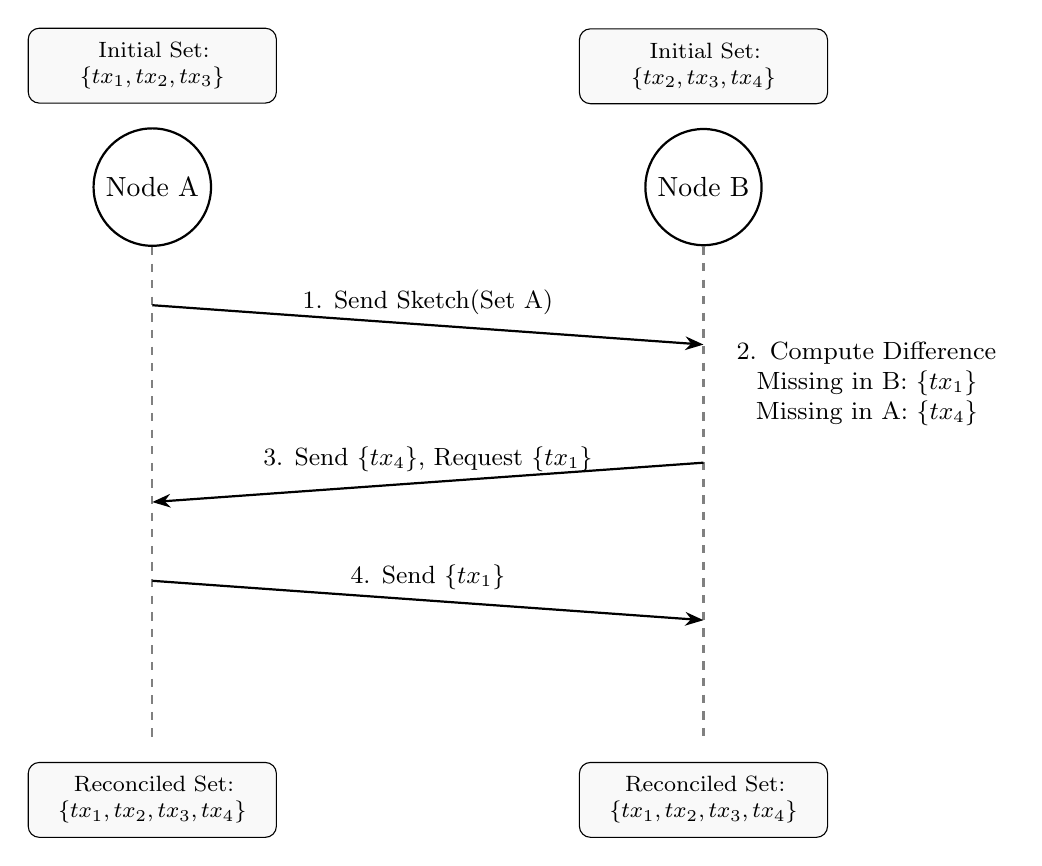
\begin{tikzpicture}[
        >=Stealth, 
        timeline/.style={dashed, gray, thick},
        action/.style={font=\small, align=center},
        box/.style={draw, rounded corners, fill=gray!5, text width=2.8cm, align=center, font=\footnotesize, inner sep=5pt}
    ]
        % We have two
        \node[draw, circle, thick, minimum size=1.2cm] (NodeA) at (0, 0) {Node A};
        \node[draw, circle, thick, minimum size=1.2cm] (NodeB) at (7, 0) {Node B};

        % Initial Sets
        \node[box, above=0.3cm of NodeA] {Initial Set:\\ $\{tx_1, tx_2, tx_3\}$};
        \node[box, above=0.3cm of NodeB] {Initial Set:\\ $\{tx_2, tx_3, tx_4\}$};

        % Vertical Timelines
        \draw[timeline] (NodeA) -- (0, -7);
        \draw[timeline] (NodeB) -- (7, -7);

        % Step 1: Send Sketch
        \draw[->, thick] (0, -1.5) -- (7, -2) node[midway, above, action] {1. Send Sketch(Set A)};

        % Step 2: Compute Difference (Bob's side)
        \node[anchor=west, action, text width=3.5cm] at (7.2, -2.5) {
            2. Compute Difference\\ 
            Missing in B: $\{tx_1\}$\\
            Missing in A: $\{tx_4\}$
        };

        % Step 3: Send missing & Request
        \draw[<-, thick] (0, -4) -- (7, -3.5) node[midway, above, action] {3. Send $\{tx_4\}$, Request $\{tx_1\}$};

        % Step 4: Final response
        \draw[->, thick] (0, -5) -- (7, -5.5) node[midway, above, action] {4. Send $\{tx_1\}$};

        % Final Synced Sets
        \node[box, below=0.3cm] at (0, -7) {Reconciled Set:\\ $\{tx_1, tx_2, tx_3, tx_4\}$};
        \node[box, below=0.3cm] at (7, -7) {Reconciled Set:\\ $\{tx_1, tx_2, tx_3, tx_4\}$};

    \end{tikzpicture}
    \caption{
        A simplified sequence diagram of set reconciliation. 
        Instead of sending full transaction lists, nodes exchange compact mathematical sketches 
        to efficiently compute the symmetric difference and synchronize their states.
    }
    \label{fig:set-reconciliation}
\end{figure}

As illustrated in \autoref{fig:set-reconciliation}, set reconciliation allows two nodes 
to synchronize their data by exchanging compressed \term{sketches}. 
When comparing these sketches, nodes can calculate the symmetric difference 
between their states and request only the specific missing messages and therefore reduce bandwidth usage.

The application of this technology to the \gls{ln} has been considered since the 
network's early days, as seen by \citeauthor{russel_diyhplus_2018}'s initial 
mailing list proposals in \citeyear{russel_diyhplus_2018}~\cite{russel_diyhplus_2018}. 
The concept was later refined by \citeauthor{myers_magical_2022} in the \term{Magical Minisketch} proposal~\cite{myers_magical_2022}. 
Most recently, active research has resumed on the \textit{Delving Bitcoin} forum, 
where developers like \citeauthor{harvey-buschel_jharveyb_2026} are developing custom tools (namely \tech{gossip-observer}) 
to gather the empirical data necessary to design a Minisketch-based gossip architecture~\cite{harvey-buschel_jharveyb_2026}.


\section{The Role of Lightning in the Bitcoin Ecosystem}
\label{sec:the-role-of-ln}

We take a step back and look at Bitcoins goal to be classified as money.
For that, an asset must fulfil the following three functions. 
It must serve as a \textit{Medium of Exchange}, a \textit{Unit of Account}, and a \textit{Store of Value}~\cite{jevons_money_1875}.
The \gls{ln} as a scaling solution focuses on making Bitcoin a viable Medium of Exchange.
This last section will first present the current state of the research that focuses on the limitations of the \gls{ln}.
Further, it introduces new designs, like \gls{mpc} as well as neighbouring projects 
that present an alternative to the design of the \gls{ln}.


\paragraph{Limitations of the Bitcoin Lightning Network}

While the \gls{ln} facilitates significantly faster and cheaper payments than the 
Bitcoin base layer, its theoretical scalability is still bounded by its topology. 
The formalization of these constraints, achieved through the mathematical modelling of payment channel networks, 
has been pioneered by \citeauthor{pickhardt_mathematical_2026}~\cite{pickhardt_mathematical_2026}.
In a recent presentation, \citeauthor{pickhardt_mathematical_2026} demonstrated 
that the network's maximum throughput is constrained by the rate of infeasible payments~\cite{pickhardt_everything_2025}. 
His model reveals a trade-off between transaction size, 
routing reliability, and overall network throughput. 
For example, to maintain a \qty{90}{\percent} likelihood of feasibility for larger payments 
(up to \qty{922259}{\sat} within the professional routing network\footnote{Selected subset of \textit{central} nodes and channels in the \gls{ln}}), 
the expected bandwidth is limited at \num{70} payments per second~\cite{pickhardt_everything_2025}. 
This throughput is only one order of magnitude higher than the capacity of the underlying Bitcoin blockchain.


\paragraph{Multi Party Channels}

To overcome these structural limitations, \citeauthor{pickhardt_mathematical_2026} 
advocates for the deployment of \term{\glspl{mpc}} and channel factories. 
By allowing multiple participants to share a single on-chain \gls{utxo}.
\glspl{mpc} could scale transaction throughput by several orders of magnitude. 
The integration would require big changes to the current \gls{ln} protocol and its client implementations.
This limitation in addition to other challenges (infrastructure management, user-experience) indicates that 
further development to elevate \gls{ln} might even exist outside the current Lightning protocol itself. 


\paragraph{Emerging Second Layer Solutions}

Alternative second layer architectures have emerged to tackle liquidity and user-experience challenges.
In \citeyear{keceli_bitcoindev_2023}, \citeauthor{keceli_bitcoindev_2023} introduced \tech{Ark}~\cite{keceli_bitcoindev_2023}. 
This protocol utilizes \glspl{vtxo} to facilitate off-chain payments without requiring users to manage inbound liquidity,
which is a major friction point within the \gls{ln}. 
Multiple independent implementations of this protocol are currently in active development. 
Similarly, the \tech{Spark} protocol, developed by \citeauthor{lightspark_buildonspark_2026}~\cite{lightspark_buildonspark_2026}, 
leverages statechains alongside a shared-signing architecture to seamlessly transfer \gls{utxo} ownership off-chain.


\paragraph{Third Layer Solutions and Ecash}

Furthermore, the ecosystem is also expanding into third layer solutions that utilize the \gls{ln} as backbone. 
\tech{Cashu}, a free and open-source \term{Chaumian ecash protocol} built for Bitcoin, has gained traction. 
It utilizes the \gls{ln} as infrastructure to facilitate value exchange between \term{Mints}, 
which in turn issue \term{ecash tokens} to users. 
These tokens can be transacted offline and with perfect anonymity, 
utilizing the blind signature cryptography invented by \citeauthor{chaum_blind_1983} in \citeyear{chaum_blind_1983}~\cite{chaum_blind_1983}.


\paragraph{Outlook: Balancing Sovereignty and Convenience}

These emerging alternative protocols vary in their custody design.
Solutions like \tech{Ark}, \tech{Spark}, \tech{Cashu} claim to be self-custodial
because the user keeps unilateral exit rights to the Bitcoin base layer.
Nonetheless, their architectures require a \enquote{central} server, 
such as an Ark Service Provider (ASP), a Spark Service Provider (SSP), or a Cashu Mint
to coordinate liquidity or route payments. 

This mediated architecture stands in contrast to the \gls{ln} where
node operators maintain absolute control over their bitcoin. 
Ultimately, these developments indicate that the future of Bitcoin scaling 
might be a balance between sovereignty and convenience. 

    \newpage
    \appendix

\newpage
\printbibliography[heading=bibintoc] 

\newpage
\phantomsection % This ensures clicking the TOC link jumps to the correct page, not the page before it.
\addcontentsline{toc}{section}{List of Figures}
\listoffigures

\newpage
\phantomsection
\addcontentsline{toc}{section}{Listings}
\listoflistings
\newpage

    \printnoidxglossary[type=\acronymtype,title=Acronyms]

\end{document}
